%\documentclass{sig-alternate-05-2015}
%\documentclass[conference]{IEEEtran}
%\IEEEoverridecommandlockouts
%\usepackage{caption}
%\usepackage{subcaption}
%\usepackage[T1]{fontenc}
%\usepackage{pgfplots}
%\pgfplotsset{
%  compat=newest,
%  xlabel near ticks,
%  ylabel near ticks
%}
%\usepackage{color}
%\usepackage{booktabs}
%\usepackage{multirow}
%\usepackage{hyperref}
%\makeatletter
%\def\@copyrightspace{\relax}
%\makeatother
%\usepackage{adjustbox}
%\begin{document}
%
%\title{Deep Semi-Supervised Learning for Defect Prediction}
%
%\maketitle\begin{abstract}
%	\label{sec:abstract}
%	The problem of software defect prediction, which involves identifying likely erroneous files in a computer program or system, has recently gained much attention in software engineering community. The ability to identify defects would help developers better focus their efforts on assuring software quality. Traditional approaches for defect prediction generally begin by a feature construction step to encode the characteristics of programs, followed by a defect modeling stage that involves training a classification algorithm. However, the feature construction stage in these approaches is carried out without considering known defect labels, potentially leading to suboptimal learned features. In light of this deficiency, we propose in this paper a new deep learning approach called \emph{deep discriminative autoencoder} (DDA), which performs end-to-end training to jointly learn discriminative (latent) features and an accurate classification model for effective defect identification. Preliminary experimental results on four popular software projects show that our DDA approach significantly outperforms traditional methods on both within-project (WP) and cross-project (CP) defect prediction. In particular, our approach improves on average by 19.63\% in terms of F1 score for the WP problems. For the CP problems, DDA outperforms other methods by 18.95\% in terms of F1 score.


%Neural Networks (NN) have been known as an important data mining technique used in classification, clustering, etc. A neural network is defined by a set of input, hidden and output layer. Each layer contains several nodes depending on user requirements. There are connection between nodes in input, hidden and output layer. Those connection represent weights between nodes. 
%In this paper, we describe Backpropagation (BP) algorithm which is one of the most popular algorithm in NN. Moreover, we also discuss an advantage and disadvantage of this algorithm. Finally, we show that BP is quite often used in practice. 

% The application of information retrieval (IR) techniques to seach tasks in software engineering is made difficult by the lexical gap between search queries (i.e., natural language) and retrieved documents (i.e., programming language). We often see this case in bug and feature location, community question answering, or more generally the communication between technical personnel and non-technical stake holders in a software project. Many previous studies treated the program elements as well as bug reports based on bag-of-words features, and estimate the correlation between the bug report and program element by measuring similarity in the same lexical feature space. However, the traditional approaches often fail to capture the word meaning for either long or short duration of time.  

%Software defect prediction help developers to find bugs and prioritize their testing efforts. The traditional approaches focus on manually designing features encoding the characteristics of programs and employing different machine algorithms to construct defect prediction models. However, the manual defect features often fail to capture the semantic differences of programs, hence the prediction models may not be accurate. 
%In this paper, we propose bridging the lexical gap between programs' semantics and defect prediction features by projecting natural language statements and programming element. Specifically, we introduce semi-supervised model inspired by autoencoder to learn semantic representation of source code as well as detect program's defect. Our framework is not only learn semantic features from token vectors extracted from programs' Abstract Syntax Trees (ASTs), but also construct classification model to detect program elements containing future bug. The experimental results show that our approach significantly outperforms the traditional approaches in defect prediction problem. 


%\textcolor{red}{write something about the results}


%we introduce deep learning model to remember the long-short term behaviour of program elements as well as bug reports. Moreover, we also apply topic modeling to expanse the program elements and bug reports, the traditional IR techniques employ to estimate the relationship between program elements and bug reports. The weights combination between two proposed approaches are learned to determine the program element related to bug report.  \textcolor{red}{Talk about experimental results later}.

%\end{abstract}
%
%\printccsdesc
%\keywords{Deep learning, defect prediction, bug localization, autoencoder, semi-supervised.}
%
%\section{Introduction}
%\label{sec:introduction}
%%Recently, text retrieval ~\cite{Salton:1988:TAA:54259.54260} approaches have been widely used to support a lof of software engineering task~\cite{Unterkalmsteiner:2016:LIR:3023163.3023241, Haiduc:2013:AQR:2486788.2486898, Arnaoudova:2015:UTR:2819009.2819224}. In these approaches, the lexical gap between user queries and code is usually identified as significant issues~\cite{Poshyvanyk:10.1109/TSE.2011.84}. In bug localization 

Software defect prediction techniques~\cite{hassan2009predicting, jiang2013personalized, zimmermann2007predicting} have been developed to automatically detect defects among program elements, which in turn help developers reduce their testing efforts and minimize
%to help developers reduce their testing efforts, thus lowering 
software development costs. In a defect prediction task, one typically constructs
%Defect prediction tries to construct 
defect prediction models from software history data, and uses these models to predict whether new instances of code elements (e.g., files, changes, and methods) contain defects or any bugs. 
%Traditional approaches try to construct accurate defect prediction models following two different directions: 
Traditionally, research efforts to construct accurate defective prediction models fall into two directions:
the first direction focuses on manually designing a set of discriminative features that can represent defects more effectively; the second direction aims to build a new machine learning algorithm that improves the conventional prediction models. 

In the past, most researchers manually designed features to filter buggy source files from non-buggy files. Specifically, the features are constructed based on changes in source code (i.e., the number of lines of code added, removed, etc.), complexity of code, or understanding of source code~\cite{jiang2013personalized, e1994candidate, mccabe1976complexity, chidamber1994metrics, harrison1998evaluation}. Meanwhile, machine learning algorithms have been used to construct a defect prediction model, such as decision tree, logistic regression, and na\"{i}ve Bayes, etc~\cite{jing2014dictionary}. 
However, traditional approaches often fail to capture the semantic differences of programs since they cannot learn code structure of different semantics. 

\textcolor{red}{[what do we mean by "semantic" here? And why traditional ML cannot capture semantic differences?]} 

%McCabe et al.~\cite{mccabe1976complexity} features focus on a complexity measure for the program elements, CK features~\cite{chidamber1994metrics} based on function and inheritance counts to understand the development of software projects, whereas MOOD features~\cite{harrison1998evaluation} provide an overall assessment of a software system. The other features are constructed based on source code changes like the number of lines of code added, removed, etc.~\cite{jiang2013personalized, e1994candidate}. On the other hand, many machine learning algorithms have been widely used for software defect prediction, including decision tree, logistic regression, Naive Bayes, etc~\cite{jing2014dictionary}. However, traditional approaches fail to distinguish code regions of different semantics. 

%To bridge the gap between programs' semantic information and features used for defect prediction, 
Wang et al.~\cite{wang2016automatically} recently developed a deep belief network (DBN) model~\cite{hinton2009deep} to automatically learn embedding features that are a compressed representation of token vectors extracted from a program's abstract syntax tree (AST). The learned features are then utilized as the training input to build a defect classification model. However, in this approach, the embedding features and defect prediction model are built separately.
%builds semantic features and defect prediction model independently. 
That is, the embedding features are learned from source files in an unsupervised manner, without considering the true label of the program element. Moreover, token values are mapped to unique integer identifier without reflecting the importance of that token in the program element. Hence, the embedding features may be suboptimal for defect prediction purposes. 

To address this shortcoming, we propose a new deep learning approach named \emph{deep discriminative autoencoder} (DDA), which provides an end-to-end learning scheme to construct discriminative embedding features and accurate defect classification model in one go. Our proposed framework extends the deep autoencoder model~\cite{ng2011sparse} by augmenting additional hidden layers that map the embedding features to an output layer where the defect classification is made.
%a deep  discriminative autoencoder (DDA) approach allowing to extract semantic features and optimize the prediction model in one stage. Our proposed framework takes advantage of antoencoder~\cite{ng2011sparse} to construct DSSL model for defect prediction. 
We summarize the key contributions of this paper below:
\begin{itemize}
	\item We develop a powerful deep learning approach for defect prediction, which is trained end-to-end using a joint loss function that simultaneously takes into account the defect prediction quality and reconstruction quality of the embedding features.
	\item We conduct extensive experiments on four popular Java software projects. The results show that our approach significantly improve traditional defect prediction methods by 8.6\% and 5.4\% in terms of F1 score, for within-project and cross project defect prediction tasks respectively. 
\end{itemize}
% We propose to leverage a powerful representationlearning
%algorithm, namely deep learning, to learn
%semantic features from token vectors extracted from
%programs' ASTs automatically.
% We leverage the semantic features learned automatically
%by DBN to improve both within-project defect
%prediction (WPDP) and cross-project defect prediction
%(CPDP).
% Our evaluation results on ten open source Java projects
%show that the automatically generated semantic features
%improve both WPDP and CPDP. ForWPDP, our
%semantic features achieve an average improvement of
%precision by 14.7%, recall by 11.5%, and F1 by 14.2%
%compared to traditional features. For CPDP, our semantic
%feature based approach outperforms the stateof-
%the-art technique TCA+ [42] built on traditional
%features by 8.9% in F1.

%To bridge the gap between programs' semantic information
%and features used for defect prediction, this paper proposes
%to leverage a powerful representation-learning algorithm,
%namely deep learning [17], to learn semantic represen-
%tation of programs automatically and use the representation
%to improve defect prediction. Specically, we use Deep Belief
%Network (DBN) [16] to automatically learn features from token
%vectors extracted from programs' ASTs, and then utilize
%these features to train a defect prediction model.

%This paper makes the following contributions:
% We propose to leverage a powerful representationlearning
%algorithm, namely deep learning, to learn
%semantic features from token vectors extracted from
%programs' ASTs automatically.
% We leverage the semantic features learned automatically
%by DBN to improve both within-project defect
%prediction (WPDP) and cross-project defect prediction
%(CPDP).
% Our evaluation results on ten open source Java projects
%show that the automatically generated semantic features
%improve both WPDP and CPDP. ForWPDP, our
%semantic features achieve an average improvement of
%precision by 14.7%, recall by 11.5%, and F1 by 14.2%
%compared to traditional features. For CPDP, our semantic
%feature based approach outperforms the stateof-
%the-art technique TCA+ [42] built on traditional
%features by 8.9% in F1.


The remainder of this paper is organized as follows. Section~\ref{sec:framework} elaborates our proposed DDA approach. Section~\ref{sec:exp_results} presents our experimental results, followed by discussion on threats to validity in Section\ref{sec:threats}. Review of key related works is given in Section~\ref{sec:relatedwork}. Finally, Section~\ref{sec:conclusion} concludes this paper.

%Section~\ref{sec:relatedwork} and Section~\ref{sec:conclusion} describe the related work and conclusion of our paper. 
%provides backgrounds on defect prediction and DBN. Section 3 describes our proposed approach to learn semantic features from source code automatically, and leverage these learned features to predict defects. Section 4 shows the experimental setup. Section 5 evaluates the performance of learned semantic features. Section 6 and Section 7 present threats to our work and related work respectively. We conclude this paper in Section 8.

%Programs have well-dened syntax, which can be represented
%by Abstract Syntax Trees (ASTs) [15] and have been
%successfully used to capture programming patterns [44, 46].
%In addition, programs have semantics, which is hidden
%deeply in source code [65]. It has been shown that programs'
%semantic information is useful for tasks such as
%code completion and bug detection [15, 28, 44, 46, 60]. Such
%semantic information should also be useful for characterizing
%defects for improving defect prediction. Specically,
%in order to make accurate predictions, the features need to
%be discriminative: capable of distinguishing one instance of
%code region from another.
%However, existing traditional features cannot distinguish
%code regions of dierent semantics. Program les with
%dierent semantics can have traditional features with the
%same values. For example, Figure 1 shows two Java les,
%File1.java and File2.java, both of which contain an if
%statement, a for statement, and two function calls. Using
%traditional features to represent these two les, their feature
%vectors are identical, because these two les have the same
%source code characteristics in terms of lines of code, function
%calls, raw programming tokens, etc. However, the semantic
%information is dierent. Features that can distinguish such
%semantic dierences should enable the building of more
%accurate prediction models.
%To bridge the gap between programs' semantic information
%and features used for defect prediction, this paper proposes
%to leverage a powerful representation-learning algorithm,
%namely deep learning [17], to learn semantic represen-
%tation of programs automatically and use the representation
%to improve defect prediction. Specically, we use Deep Belief
%Network (DBN) [16] to automatically learn features from token
%vectors extracted from programs' ASTs, and then utilize
%these features to train a defect prediction model.
%
%DBN is a generative graphical model, which learns a representation
%that can reconstruct training data with a high
%probability. It automatically learns high-level representation
%of data by constructing a deep architecture [2]. We have
%seen successful applications of DBN in many elds, including
%speech recognition [37], image classication [6, 25], natural
%language understanding [35, 55], and semantic search [54].
%To use a DBN to learn features from code snippets, we
%convert the code snippets into vectors of tokens with structural
%and contextual information preserved, and use these
%vectors as input to the DBN. For the two code snippets in
%Figure 1, the input vectors will be [..., if, foo, for,
%bar, ...] and [..., foo, for, if, bar, ...] respectively.
%Since the vectors of these two les are dierent,
%DBN will automatically learn features to distinguish these
%two code snippets (details are in Figure 3 and Section 3.3).
%This paper makes the following contributions:
% We propose to leverage a powerful representationlearning
%algorithm, namely deep learning, to learn
%semantic features from token vectors extracted from
%programs' ASTs automatically.
% We leverage the semantic features learned automatically
%by DBN to improve both within-project defect
%prediction (WPDP) and cross-project defect prediction
%(CPDP).
% Our evaluation results on ten open source Java projects
%show that the automatically generated semantic features
%improve both WPDP and CPDP. ForWPDP, our
%semantic features achieve an average improvement of
%precision by 14.7%, recall by 11.5%, and F1 by 14.2%
%compared to traditional features. For CPDP, our semantic
%feature based approach outperforms the stateof-
%the-art technique TCA+ [42] built on traditional
%features by 8.9% in F1.
%The rest of this paper is summarized as follows. Section 2
%provides backgrounds on defect prediction and DBN. Section
%3 describes our proposed approach to learn semantic
%features from source code automatically, and leverage these
%learned features to predict defects. Section 4 shows the experimental
%setup. Section 5 evaluates the performance of
%learned semantic features. Section 6 and Section 7 present
%threats to our work and related work respectively. We conclude
%this paper in Section 8.
%
%
%
%\section{Proposed Approach}
%\label{sec:framework}
%\subsection{Defect Prediction}
\label{sec:defect_prediction}
%\begin{figure*}[t!]
%	\centering
%	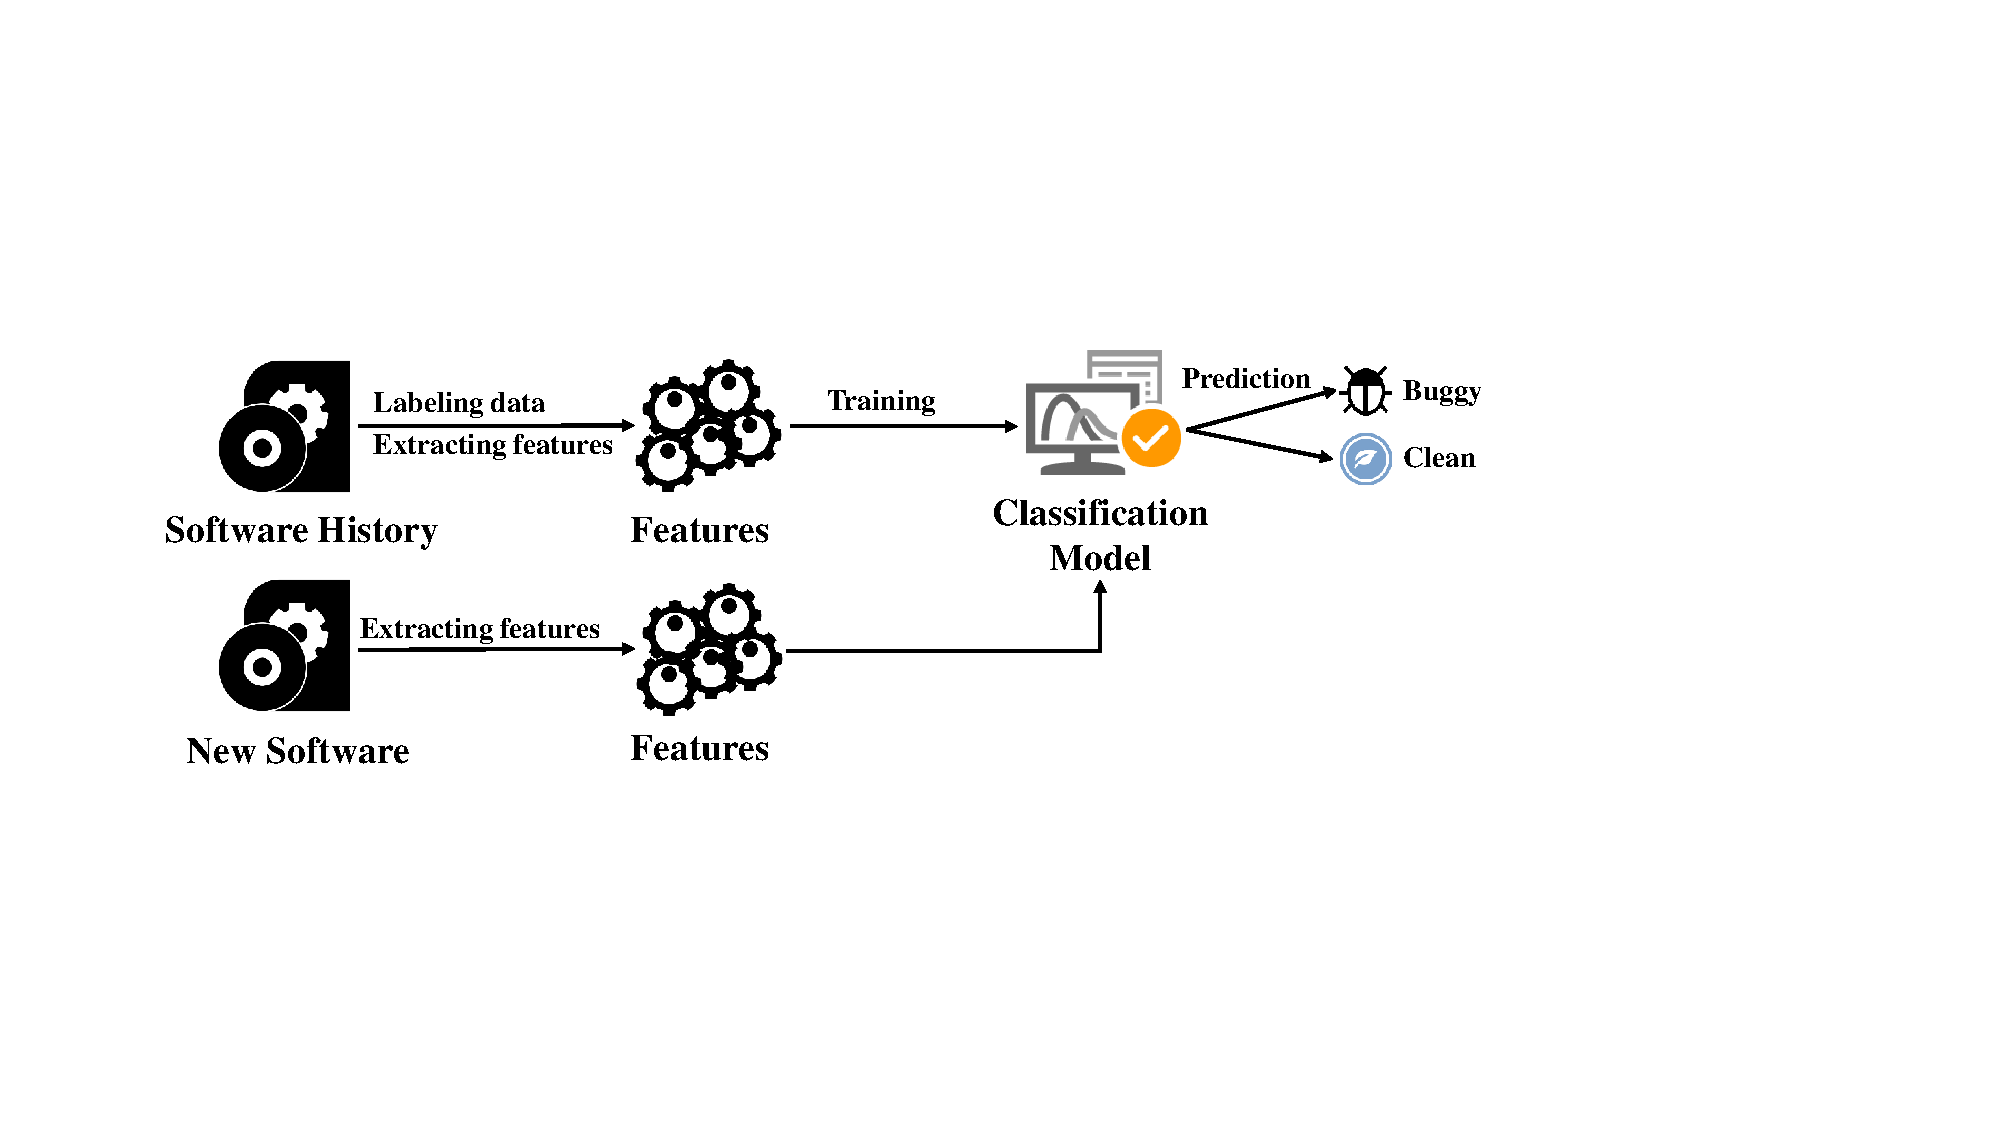
\includegraphics[width=0.85\textwidth]{defect_framework}
%	\caption{Defect Prediction Framework}
%	\label{fig:defect}
%\end{figure*}
\begin{figure}
	\centering
	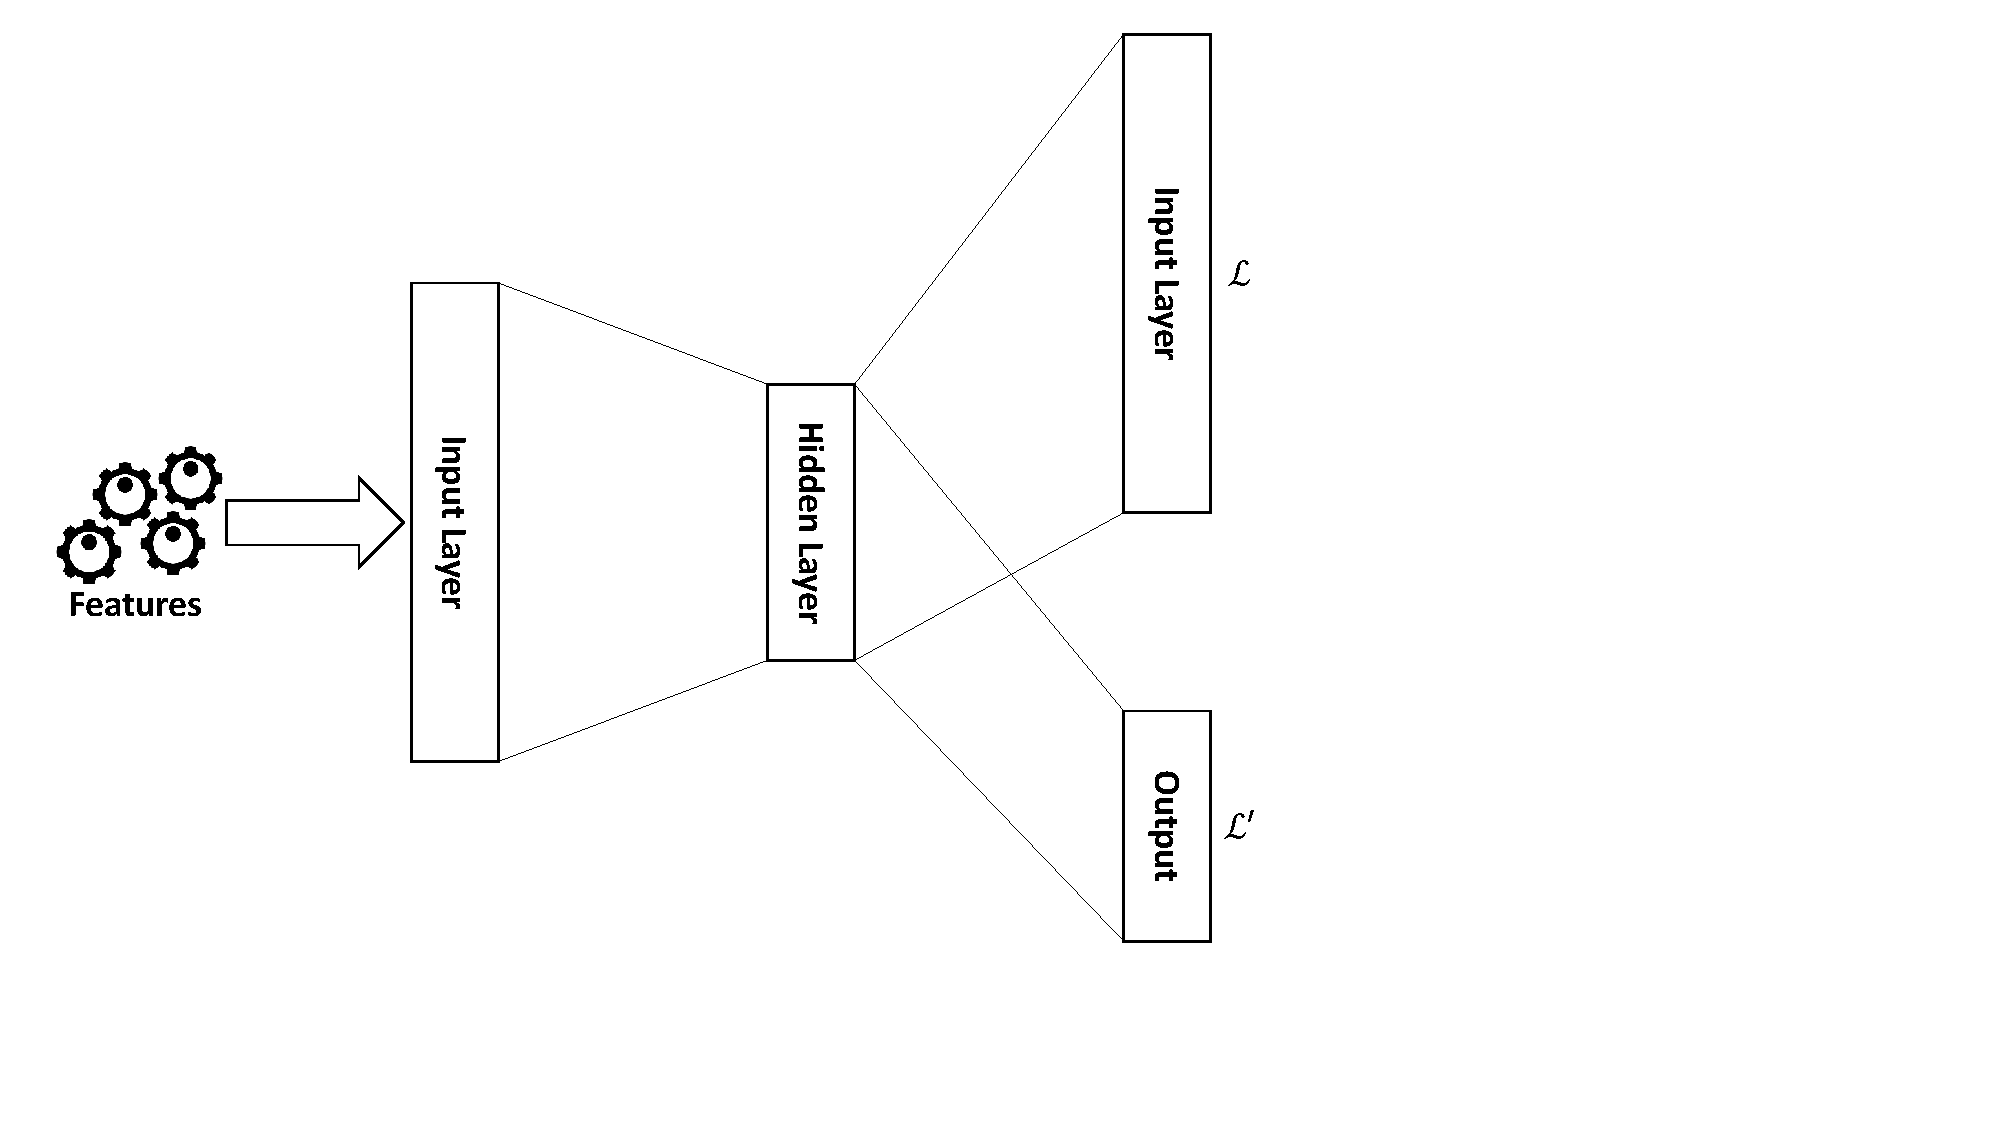
\includegraphics[width=0.45\textwidth]{dssl_framework}
	\caption{Deep Semi-supervised Learning Framework}
	\label{fig:semi_framework}
\end{figure}


%Figure~\ref{fig:defect} presents the overall framework of file-level defect prediction. Typically, the defect prediction problem is solved by following two specific steps. 
The overall process of our file-level defect prediction follows two specific steps. The first step is to label source code files as buggy or clean and then extracts traditional features of these files. These traditional features are introduced in~\cite{wang2016automatically, mccabe1976complexity, chakradeo2013mast}. The second step is to construct a defect prediction model~\cite{bishop2006pattern} to predict whether a new source code file is buggy or clean.  We refer to the software version used for building our defect prediction model as training data and the one used to evaluate the built model as testing data. 

%Figure 2 presents a typical le-level defect prediction process
%that is adopted by existing studies [20,27,34,41,42,51,
%64]. The rst step is to label data as buggy or clean based
%on post-release defects for each le. A le is buggy if the le
%contains bugs. Otherwise, the le is clean. The second step
%is to collect corresponding traditional features of these les.
%Instances with features and labels are used to train machine
%learning classiers. Finally, trained models are used to predict
%new instances as buggy or clean.
%We refer to the set of instances used for building models as
%the training set, whereas the set of instances used to evaluate
%the trained models as the test set. As shown in Figure 2,
%when performing within-project defect prediction (following
%existing work [41], we call this WPDP), the training and test
%sets are from the same project A. When performing crossproject
%defect prediction (following existing work [41] we call
%this CPDP), prediction models are trained by training set
%from a project A (source), and test set is from a dierent
%project B (target).
%In this study, we examine the performance of learned semantic
%features on both WPDP and CPDP.

\subsection{Parsing Source Code and Generating Features}
\label{sec:parsing}
%In our approach, we follow Wang et al.~\cite{wang2016automatically} to extract source code information to learn semantic features. Typically, the syntactic information from source code is collected based on Java Abstract Syntax Tree (AST)~\cite{neamtiu2005understanding}. For each program element, we extract a vector of tokens of the three types of AST nodes: 1) nodes of method invocations and class instance creations, 2) declaration nodes, i.e., method declarations, type declarations, etc. and 3) control-flow nodes such as while statements, catch clauses, if statements, for statements, etc. Note that our semi-supervised learning only takes numerical vectors as inputs, and the lengths of the input vectors are the same. Thus, we apply Wang approaches~\cite{wang2016automatically} to map between integers and tokens, and encode token vectors to integer vector. Note that our integer vectors may have different lengths, we append 0 to the integer vectors to make all the lengths consistent and equal to the length of the longest vector. We also note that adding zeros does not affect the results, since it is simply representation transformation to make the vectors acceptable by neural network~\cite{wang2016automatically}.

In our approach, we follow Wang et al.~\cite{wang2016automatically} approach to extract source code information. Typically, the syntactic information from source code is collected based on Java Abstract Syntax Tree (AST)~\cite{neamtiu2005understanding}. For each Java source code file, we extract a sequence of AST node tokens of these types: 1) nodes of method invocations and class instance creations, 2) declaration nodes, i.e., method declarations, type declarations, and enum declarations, and 3) control-flow nodes such as while statements, catch clauses, if statements, for statements, etc. Unlike Wang approach which encode the extracted tokens as unique integers and use them as features, we encode the tokens using a term frequency - inverse document frequency (TF-IDF)~\cite{manning2008introduction} and consider them as features for our framework (i.e., deep semi-supervised learning). These features reflects how important a token is in its corresponding source code file.

%Note that our semi-supervised learning only takes numerical vectors as inputs, and the lengths of the input vectors are the same. Thus, we apply Wang approaches~\cite{wang2016automatically} to map between integers and tokens, and encode token vectors to integer vector. Note that our integer vectors may have different lengths, we append 0 to the integer vectors to make all the lengths consistent and equal to the length of the longest vector. We also note that adding zeros does not affect the results, since it is simply representation transformation to make the vectors acceptable by neural network~\cite{wang2016automatically}.

%DBN takes only numerical vectors as inputs, and the
%lengths of the input vectors must be the same. To use DBN
%to generate semantic features by using DBN, we rst build
%a mapping between integers and tokens, and encode token
%vectors to integer vectors. Each token has a unique integer
%identier while dierent method names and class names will
%be treated as dierent tokens. Since our integer vectors may
%have dierent lengths, we append 0 to the integer vectors
%to make all the lengths consistent and equal to the length
%of the longest vector. Adding zeros does not aect the
%results, and it is simply a representation transformation to
%make the vectors acceptable by DBN. Taking code snippets
%in Figure 3 as an example, if we consider only \File1" and
%\File2", the token vectors for \File1" and \File2" would be
%mapped to [1, 2, 3, 4] and [2, 3, 1, 4] respectively. Through
%this encoding process, method invocation information and
%inter-class information are represented as integer vectors. In
%addition, some program structure information is preserved
%since the order of tokens remains unchanged.


\subsection{Deep Semi-supervised Learning}
\label{sec:semi}
The goal of defect prediction is to detect source code files that may contain bug in the future. 

Let $\mathcal{X}=\{x_1, x_2, \dots, x_n\}$ denotes the set of source code files in a software project and $\mathcal{Y}=\{y_1, y_2, \dots, y_n\}$ represents the set of labels for the source code files, where $n$ is the number of source code files in the project.  Note that the source code file is labeled as $1$ if it contains bug, otherwise it will be labeled as $0$ which means that it is clean from bug. %The source files can be collected from github repository~\footnote{https://github.com/}
%The source files can be collected from some popular software projects (e.g, ant, camel, lucene, etc.)~\footnote{http://openscience.us/repo/defect/}. 
Unlike traditional approaches~\cite{yang2015deep, wang2016automatically} that independently learn semantic features and construct defect prediction model, our deep semi-supervised learning (DSSL) combines the two tasks for tackling the defect prediction problem. Typically, we attempt to learn a semantic features function $f: \mathcal{X} \longmapsto \mathcal{X}$ and a defect prediction function $f': \mathcal{X} \longmapsto \mathcal{Y}$, $y_i \in \mathcal{Y}=\{0, 1\}$ indicates whether a source code file $x_i \in \mathcal{X}$ contains a bug. % which can be obtained by investigating software commit logs and bug report descriptions~\cite{fischer2003populating}.
These two functions $f$ and $f'$ can be learned by minimizing the following objective function:
%We formalize the our approaches as a joint optimization, expressed by the loss function $\mathcal{L}$, for learning semantic features and building defect prediction model as following:
\begin{equation}
\label{eq:loss}
\begin{split}
\min_{f,f'} \sum_{i}^{}\mathcal{L}(f(x_i), x_i) + \theta \mathcal{L'}(f'(x_i), y_i) \\
+ \lambda \Omega(f, f')
\end{split}
\end{equation}
where $\mathcal{L}(\cdot, \cdot)$ and $\mathcal{L}'(\cdot, \cdot)$ are the empirical loss of the semantic features and the defect prediction functions, respectively. $\theta$ is the predefined value for weighting the two loss functions. $\Omega(f, f')$ is the regularization term imposed on the two functions. The trade-off between the empirical loss and the regularization term is controlled by $\lambda$. 

The overall framework of DSSL is shown in Figure~\ref{fig:semi_framework}. The DSSL model contains three different layers: input layer, hidden layer, and output layer. Given a source code file, the features extracted in Section~\ref{sec:parsing} are fed to the input layer while the corresponding defect label is fed to the output layer. The network consisting of input layer, hidden layer, and input layer represents an encoder-decoder model. The encoder-decoder model is required to learn semantic features. Note that our encoder-decoder model are inspired by autoencoder~\cite{ng2011sparse}, which is an unsupervised learning technique. The original autoencoder only learn the function $f: \mathcal{X} \longmapsto \mathcal{X}$ so that the output values $\mathcal{\hat{X}}$ are similar to input values $\mathcal{X}$. On the other hand, DSSL attempts to learn semantic features and optimize defect prediction task, thus it takes into account two functions, i.e., $f$ and $f'$, which represents the semantic features and defect prediction function, respectively. $f'$ is learned through the connection between the hidden layer and the output layer. According to Figure~\ref{fig:semi_framework}, our model optimizes two loss functions, i.e., $\mathcal{L}$ and $\mathcal{L'}$ to construct the defect prediction model. In encoder-decoder model, we employ a fully connected neural network for learning to convert low level features from source code files to semantic features. At the same time, our network learns to determine on whether the given source code file is buggy based on the semantic features. 

%The overall framework of DSSL is shown in Figure~\ref{fig:semi_framework}. The DSSL model contains two four different parts: parsing abstract syntax tree, generating features, encoder, and decoder. The first two steps are briefly described in Section~\ref{sec:parsing} to feed source files data to our deep neural network. Encoder and decoder are required to learn semantic features as well as defect prediction model. Note that our encoder and decoder steps are inspired by autoencoder~\cite{ng2011sparse} which is an unsupervised learning technique. However the original autoencoder only tries to learn the function $f: \mathcal{X} \longmapsto \mathcal{X}$ so that the output values $\mathcal{\hat{X}}$ are similar to input values $\mathcal{X}$. However, SSA attempts to learn semantic features and optimize defect prediction model, thus it takes into account of two functions, i.e., $f$ and $f'$ represent the semantic features and defect prediction respectively. According to Figure~\ref{fig:semi_framework}, our model tries to optimize two different loss functions, i.e., $\mathcal{L}$ and $\mathcal{L'}$ to construct the defect prediction model. In encoder and decoder steps, we employ a fully connected neural network to fuse middle-level features extracted from source files to generate semantic features, where our network is learn to facilitate the determination on whether the given source code file is related to the given bug report based on the semantic features. In this paper, we employ Adam optimization~\cite{kingma2014adam}, which is popular optimization method in deep learning community, to optimize the two loss functions for constructing defect prediction model. 

%In the cross-language feature fusion layers, we employ a fully connected neural network to fuse middle-level features ex- tracted from bug reports and source files to generate a unified feature representation, where the network is learned in order to facilitate the determination on whether the given source code file is related to the given bug report based on the uni- fied feature.


%To learn semantic features from program elements, we employ autoencdoer

%Ω(f) is a regulariza- tion term imposing on the prediction function. The trade-off between L(·, ·) and Ω(f ) is balanced by λ.

%Let C = fc1; c2;    ; cN1g denotes the set of source code
%files of a software project andR = fr1; r2;    ; rN2g denotes
%the collection of bug reports received by the software maintenance
%team, where N1;N2 are the number of source files and
%bug reports, respectively. The bug reports and source files can
%be collected from bug tracking systems (e.g., Bugzilla, Jira,
%etc.) and history control systems (e.g., CVS, Git, etc.).

\subsection{Imbalanced Problem in Defect Prediction}
\label{sec:imbalanced}
In defect prediction tasks, often times there are only a few source code files that contain bugs while the other source code files are \textit{clean}~\cite{khoshgoftaar2010attribute}. This consequently makes the labeled data to be imbalanced. This imbalanced nature increases the learning difficulty. For this reason, imbalanced class learning, which specializes in tackling classification problems involving imbalanced data, is helpful for defect prediction problem~\cite{wang2013using}. To address this imbalanced data issue, we propose a balanced random sampling procedure when picking a data instance to update our DSSL network weights. In particular, we select a random instance from each the positive and negative instance pools to mitigate the issue of skewed distribution. This mitigates the issue of imbalanced data in defect prediction. 


%To address this problem, we propose to learn the semantic features that may counteract the negative influence of the imbalanced data in the subsequent learning of defect prediction function. Inspired by~\cite{zhou2006training}, we introduce an unequal misclassification cost according to the imbalance ratio and train the fully connected network in a cost-sensitive manner. 
%
%Let $r_n$ denote the ratio cost of incorrectly associating an \textit{clean} source code file to a bug program element and $r_p$ denote the cost of missing a buggy source code file in the training data. The weight of the semi-supervised autoencoder (SSA) networks $\mathcal{W}$  can be learned by minimizing the following objective function following Adam optimization~\cite{kingma2014adam}. 
%\begin{equation}
%\label{eq:imbalanced}
%\begin{split}
%\min_{\mathcal{W}} \sum_{i}^{}\mathcal{L}(f(x_i), x_i) 
%+ r_n \mathcal{L}'(x_i, y_i;\mathcal{W}) y_i \\ + r_p \mathcal{L}'(x_i, y_i;\mathcal{W}) (1 - y_i) + \lambda \rVert \mathcal{W} \rVert^2
%\end{split}
%\end{equation}
%where $\mathcal{L}$ and $\mathcal{L}'$ are the loss function for semantic features and defect prediction model, respectively. $\lambda$ is the trade-off parameter.  
%To address this, we devise a balanced random
%sampling procedure when picking a data instance for gradient
%descent update. In particular, for every update step, we
%alternatingly select a random instance from the positive and
%negative instance pools, as per lines 4-8 of Algorithm 1.
%Using this simple method, we can balance the training
%from positive and negative instances, thus effectively mitigating
%the issue of skewed distribution in the localization
%task. It is also worth noting that our iterative tuning procedure
%is efficient. That is, its time complexity is linear with
%respect to the number of instances N and maximum iterations
%Tmax.


%Let costn denote the cost of incorrectly associating an ir- relevant source code file to a bug report and costp denote the cost of missing a buggy source code file that is responsible for the reported bugs. The weight of the fully connected net- works w can be learned by minimizing the following objec- tive function based on SGD (stochastic gradient descent).

%the imbalanced nature of this type of data increases the learning difficulty of such a task. Class imbalance learning specializes in tackling classification problems with imbalanced distributions, which could be helpful for defect prediction, but has not been investigated in depth so far. In this paper, we study the issue of if and how class imbalance learning methods can benefit software defect prediction with the aim of finding better solutions.    



%In the cross-language feature fusion layers, we employ a fully connected neural network to fuse middle-level features ex- tracted from bug reports and source files to generate a unified feature representation, where the network is learned in order to facilitate the determination on whether the given source code file is related to the given bug report based on the uni- fied feature.
%In most cases of bug localization, a reported bug may be only related to one or only a few source code files, while a large number of source code files are irrelevant to the given bug report. Such an imbalance nature increases the difficulty in learning a well-performing prediction function based on the unified feature.
%To address this problem, we propose to learn the unified feature that may counteract the negative influence of the im- balanced data in the subsequent learning of prediction func- tion. Inspired by [Zhou and Liu, 2006], we introduce an un- equal misclassification cost according to the imbalance ratio and train the fully connected network in a cost-sensitive man- ner.
%Let costn denote the cost of incorrectly associating an ir- relevant source code file to a bug report and costp denote the cost of missing a buggy source code file that is responsible for the reported bugs. The weight of the fully connected net- works w can be learned by minimizing the following objec- tive function based on SGD (stochastic gradient descent).

\subsection{Setting for Training Deep Semi-supervised Learning}
\label{sec:setting}
In our setting, the number of hidden layers, the number of nodes in each hidden layer, the number of iterations, and $\theta$ are chosen by performing cross validation on training data. By default, the number of hidden layers, the number of nodes in each hidden layer, and number of iteration are selected as 2, 1000-100, and 75, respectively. We employ Adam optimization~\cite{kingma2014adam}, which is popular optimization method in deep learning community, to optimize the two loss functions for constructing DSSL. %Note that $\theta$ in Equation~\ref{eq:loss} is also well-chosen based on training data to solving imbalanced between two loss functions. 


%Some deep learning application~\cite{hinton2009deep, ng2011sparse} reports an effective of deep learning models need well-tuned parameters, i.e., 1) the number of hidden layers, 2) the number of nodes in each hidden layer, and 3) the number of iterations.
%In our deep semi-supervised learning, we choose two hidden layers and  these parameters are chosen by learning from training data 
%
% In~\cite{wang2016automatically}, the authors pointed out that the deep learning model was optimized when they chose 10, 100, 200 as the number of hidden layers, number of nodes in each hidden layer, and number of iterations respectively. For the fair comparison with~\cite{wang2016automatically}, we use these parameters to train our deep semi-supervised learning model. 

%Many DBN applications [6,25,37] report that an eective
%DBN needs well-tuned parameters, i.e., 1) the number of hid-
%den layers, 2) the number of nodes in each hidden layer, and
%3) the number of iterations. In this study, since we leverage
%DBN to generate semantic features, we need to consider the
%impact of the three parameters. We tune the three parameters
%by conducting experiments with dierent values of the
%parameters on ant (1.5, 1.6), camel (1.2, 1.4), jEdit (4.0,
%4.1), lucene (2.0, 2.2), and poi (1.5, 2.5) respectively. Each
%experiment has specic values of the three parameters and
%runs on the ve projects individually. Given an experiment,
%for each project, we use the older version of this project to
%train a DBN with respect to the specic values of the three
%parameters. Then, we use the trained DBN to generate semantic
%features for both the older and newer versions. After
%that, we use the older version to build a defect prediction
%model and apply it to the newer version. Lastly, we evaluate
%the specic values of the parameters by the average F1 score
%of the ve projects in defect prediction.




%
%\section{Experimental Results}
%\label{sec:exp_results}
%We conduct extensive experiments to study the performance of the proposed approach and compare it with existing defect prediction approaches. We also discuss threats to the validity of our approach.

\subsection{Evaluation Metrics}
\label{sec:metrics}
To measure defect prediction results, we employ three different metrics: \textit{Precision}, \textit{Recall} and \textit{F1}. These evaluation metrics are widely used to evaluate the performance of defect prediction~\cite{menzies2007data, menzies2010defect, nam2013transfer} as well as information retrieval binary classification~\cite{manning2008introduction}. Typically, precision is the fraction of retrieved instances that are relevant, recall is the fraction of relevant instances that are retrieved, whereas F1 combines both precision and recall to measure the performance of our model. Below is the equation of these metrics:
\begin{equation}
\label{eq:precision}
Precision = \frac{TP}{TP+FP}
\end{equation}

\begin{equation}
\label{eq:recall}
Recall = \frac{TP}{TP+FN}
\end{equation}

\begin{equation}
\label{eq:f1}
F1 = \frac{2 * Precision * Recall}{Precision + Recall}
\end{equation}
where \textit{TP}, \textit{FP}, and \textit{FN} are considered as true positive, false positive, and false negative respectively. True positive is the number of predicted defective files that are truly defective, while false positive is the number of predicted defective files that are actually not defective. False negative records the number of predicted non-defective files that are actually defective. A higher precision makes the manual inspection on a certain amount of predicted defective files find more defects, while an increase in recall can reveal more defects given a project. F1 takes consideration of both precision and recall.


\subsection{Datasets}
\label{sec:dataset}

\textcolor{red}{Ferdian: Can you help me to rewrite dataset section?}

We perform several steps to create our benchmark dataset. Firstly, we fetch top 2,500 most popular open-source Java projects from GitHub (sorted by the sum of their number of stars and number of forks). GitHub contains many toy projects, thus, we only consider popular projects similar to prior studies~\cite{ray2014large, kochhar2016large}. We only clone the git repositories of projects which use Maven as we leverage Maven to automatically build the projects and construct call graphs from compiled classes. Out of the 2500 projects, 831 projects use Maven. Secondly, we collect 342 Apache Java projects which use Maven and are hosted on GitHub. A er removing the overlapping projects, our dataset contains 1,143 projects.

Next, we ignore projects with less than 150 source files as these projects are too small to employ deep neural netwok. We also  filter out projects which have less than 100 tested files. For each project, we have two versions: current version (i.e., latest version as of June 2016) which serves as a test dataset, and previous version (i.e., version one year prior to current version) which serves as a training set. We compile these two versions using \textit{mvn compile:compile}. We ignore projects whose current and/or previous version cannot be compiled. In the end, our dataset has 28 projects.

Table~\ref{tab:data} shows the overview of our dataset containing 28 projects. In average, our data has around 921 source files in training set and more than 1020 program elements in testing set. Average bug rate is 18.7\% and 7.5\% on training and testing data respectively showing the imbalanced problem in defect prediction~\cite{wang2013using, khoshgoftaar2010attribute}. 

%having a total of 46 million SLOC, 83 thousand source code  les, 0.9 million methods, 280 thousand commits and over 45 thousand test  les contributed by more than 5 thousand developers spanning over period of 15 years, i.e., 2001-2016. Our dataset con- tains popular projects such as Apache Commons IO [4], which is a library of utilities for IO functionalities and Joda-Time [31], which is date and time library for Java.

\subsection{Baselines}
\label{sec:baselines}
%To evaluate the performance of our approach in defect prediction, we compare with traditional features (see Section~\ref{sec:relatedwork}). The first baseline consists some traditional features, including lines of code, cyclomatic complexity~\cite{mccabe1976complexity}, total number of methods, total number of public methods, total number of local methods, the depth of inheritance tree, comment density, etc. These features are well described in~\cite{hassan2009predicting} and have been widely used in previous work~\cite{jing2014dictionary, menzies2007data, menzies2010defect, nam2013transfer, zimmermann2007predicting, yang2015deep}. Since they are popular features so we can directly compare our work with previous studies. We note that the traditional features do not contain Abstract Syntax Tree (AST) nodes, which are described in this paper. 

We compare our approach with the defect prediction models constructed based on two traditional features. The first traditional features are embedding features generated following Wang et al.~\cite{wang2016automatically}. The second traditional features are AST features extracted from source code's AST. Specifically, we collect AST nodes from source code and represent the source code as a vector of term frequencies of the AST nodes. These two baselines were shown their effectiveness in solving defect prediction problem~\cite{wang2016automatically}.

%To evaluate the performance of our approach in defect prediction, we compare it with traditional defect prediction models that are constructed using the state-of-the-art semantic features learning approach by Wang et al.~\cite{wang2016automatically}. They employ Deep Belief Network~\cite{hinton2009deep} to automatically learn semantic features from token vectors extracted from source code's AST. They have shown that their semantic features significantly improve the performance of defect prediction. 

%The second baseline includes semantic features constructed following Wang et al. approaches~\cite{wang2016automatically}. Typically, they tried to employ deep belief network~\cite{hinton2009deep} to automatically learn semantic features from token vectors extracted from programs' AST. They also proved that their semantic features significantly improve the performance of defect prediction in software engineering domain. 

We employ three popular machine learning algorithms~\cite{bishop2006pattern} to build defect prediction models for each traditional features. These algorithms are widely used in software engineering~\cite{wang2016automatically, wang2013using, jing2014dictionary} described as follows: 
\begin{itemize}
%	\item Decision tree is used to build a tree-based predictive model where branch nodes represent an option on feature values while leaf nodes represent predicted values. Tree models in which the predicted values are taken from a finite set are called classification trees. In these tree structures, leaf nodes represent class labels and branch node sequences represent conjunctions of features that lead to those class labels. This algorithm is very popular in statistics, data mining and machine learning~\cite{safavian1991survey}.
	\item Decision tree is used to build a tree-based classification model where branch nodes represent an option on feature values while leaf nodes represent predicted values~\cite{safavian1991survey}.
%	\item Logistic regression is a predictive model that explains the relationship between one dependent binary variable and one or more nominal, ordinal, interval or ratio-level independent variables. Logistic regression is used in various applications like: health, statistics, data analysis, etc.~\cite{hosmer2013applied}.
	\item Logistic regression is a well-known classification model that employs in various application such as: health, statistics, data analysis, etc.~\cite{hosmer2013applied}. 
%	explains the relationship between one dependent binary variable and one or more nominal, ordinal, interval or ratio-level independent variables. Logistic regression is used in various applications like: health, statistics, data analysis, etc.~\cite{hosmer2013applied}.
	\item Na\"{i}ve Bayes classifier, which are highly scalable, is a simple probabilistic classifiers based on applying Bayes' theorem ~\cite{vapnik1998statistical}. 
%	with strong (naive) independence assumptions between the features. Naive Bayes classifiers are highly scalable, requiring only a number of parameters that is linear with the number of variables (features/predictors). For some types of probability models, Naive Bayes classifiers can be trained very efficiently in a supervised learning setting. In many practical applications, parameter estimation for Naive Bayes models uses the method of maximum likelihood~\cite{pan2002maximum}.
\end{itemize}

%The 20 traditional features are available for PROMISE data, and the work from He et al. [13] contains the full list of the 20 features, which are well described in their Table II. These features and data have been widely used in previous work [20, 33, 34, 42, 70]. We choose the widely used PROMISE data so that we can directly com- pare our work with previous studies. Note that, for a fair comparison, we also perform the noise removal approach de- scribed in Section 3.2.1 on the PROMISE data.


%The traditional features from PROMISE do not contain AST nodes, which were used by our DBN models. For a fair comparison, our second baseline of traditional features is the AST nodes that were given to our DBN models, i.e., the AST nodes in all files after fixing noise (Section 3.2.1). Each instance is represented as a vector of term frequencies of the AST nodes.

%To bridge the gap between programs' semantics and
%defect prediction features, this paper proposes to leverage a
%powerful representation-learning algorithm, deep learning,
%to learn semantic representation of programs automatically
%from source code. Specically, we leverage Deep Belief
%Network (DBN) to automatically learn semantic features
%from token vectors extracted from programs' Abstract
%Syntax Trees (ASTs).
%Our evaluation on ten open source projects shows that
%our automatically learned semantic features signicantly improve
%both within-project defect prediction (WPDP) and
%cross-project defect prediction (CPDP) compared to traditional
%features. Our semantic features improve WPDP on
%average by 14.7% in precision, 11.5% in recall, and 14.2%
%in F1. For CPDP, our semantic features based approach
%outperforms the state-of-the-art technique TCA+ with traditional
%features by 8.9% in F1.

% Table generated by Excel2LaTeX from sheet 'WithinProjects'
\begin{table*}[t!]
	\centering
	\caption{
%		Comparison between DDA and three classification algorithms (decision tree, logistic regression, and na\"{i}ve Bayes) using semantic features and AST features. P, R, and F1 denote precision, recall and F1 score respectively and are measured by percentage. The best F1 scores are highlighted in bold.
		Precision, recall and F1 scores of within-project prediction. All the scores are measured by percentage. The best F1 scores are highlighted in bold. Deep discriminative autoencoder, decision tree, logistic regression, and na\"{i}ve Bayes are denoted as DDA, DT, LR, NB respectively. 
	}
	\begin{adjustbox}{width=1\textwidth}
	\begin{tabular}{|c|c|c|c|c|c|c|c|}
		\hline
		\multirow{3}[6]{*}{Project} & \multirow{2}[4]{*}{DDA} & \multicolumn{3}{c|}{Embedding} & \multicolumn{3}{c|}{AST} \\
		\cline{3-8}          &       & DT    & LR    & NB    & DT    & LR    & NB \\
		\cline{2-8}          & P R F1 & P R F1 & P R F1 & P R F1 & P R F1 & P R F1 & P R F1 \\
		\hline
		\hline
		\multicolumn{1}{|l|}{Checkstyle} & 74.6 84.7 \textbf{79.3} & 78.3 55.3 64.8 & 83.6 68.8 75.5 & 72.3 82.9 77.3 & 82.4 63.5 71.8 & 79.7 62.4 70.0  & 82.7 64.7 72.6 \\

		\multicolumn{1}{|l|}{Nuvolabase} & 33.8 66.0 \textbf{44.7} & 32.8 7.51 12.2 & 36.2 44.7 40.0 & 31.1 73.5 43.7 & 50.7 14.2 22.2 & 59.6 12.2 20.3  & 20.3 41.1 27.1 \\
		
		\multicolumn{1}{|l|}{OrientDB} & 32.9 47.9 \textbf{39.0} & 25.6 6.94 10.9 & 27.3 47.2 34.6 & 20.8 69.4 32.0 & 40.3 18.8 25.6 & 44.2 13.2 20.3  & 12.1 38.2 18.4 \\
		
		\multicolumn{1}{|l|}{Traccar} & 33.9 75.0 \textbf{46.7} & 14.0 80.0 23.9 & 12.7 75.0 21.7 & 12.8 95.0 22.0 & 20.0 20.0 20.0 & 12.2 70.0 20.7  & 9.47 90.0 17.1 \\
		\hline
		\hline
		Average & 43.8 68.4 \textbf{52.4} & 37.7 37.4 28.0 & 39.9 58.9 42.9 & 34.3 80.2 43.8 & 48.4 29.1 34.9 & 48.9 39.5 32.8 & 31.1 58.5 33.8 \\
		\hline
	\end{tabular}%
	\end{adjustbox}
	\label{tab:within}%
\end{table*}%


% Table generated by Excel2LaTeX from sheet 'CrossProjects'
\begin{table}[t!]
	\centering
	\caption{Precision, recall and F1 scores of cross-project defect prediction. All the scores are measured by percentage. The best F1 scores are highlighted in bold.}
	\begin{adjustbox}{width=0.48\textwidth}
	\begin{tabular}{|c|c|c|c|c|}
		\hline
		\multirow{3}[6]{*}{Source } & \multirow{3}[6]{*}{Target} & \multicolumn{2}{c|}{Cross-project} & \multirow{2}[4]{*}{Within-project} \\
		\cline{3-4}          &       & DDA & Embedding &  \\
		\cline{3-5}          &       & P R F1 & P R F1 & P R F1 \\
		\hline
		\hline
		\multicolumn{1}{|l|}{Nuvolabase} & \multicolumn{1}{l|}{Checkstyle} & 79.0 57.6 \textbf{66.7} & 54.5 38.8 45.3  & \multirow{2}[4]{*}{74.6 84.7 79.3} \\
		\cline{1-4}    \multicolumn{1}{|l|}{OrientDB} & \multicolumn{1}{l|}{Checkstyle} & 94.3 29.4 44.8 & 54.7 48.2 \textbf{51.3} &  \\
		\hline
		\multicolumn{1}{|l|}{Checkstyle} & \multicolumn{1}{l|}{Nuvolabase} & 45.5 36.4\textbf{ 40.4} & 27.0 52.2 35.6 & \multirow{2}[4]{*}{33.8 66.0 44.7} \\		
		\cline{1-4}    \multicolumn{1}{|l|}{Traccar} & \multicolumn{1}{l|}{Nuvolabase} & 44.2 36.4 \textbf{40.0} & 27.1 41.5 32.8 &  \\
		\hline
		\multicolumn{1}{|l|}{Nuvolabase} & \multicolumn{1}{l|}{OrientDB} & 57.1 16.7\textbf{ 25.8}  & 16.2 31.9 21.5 & \multirow{2}[4]{*}{32.9 47.9 39.0} \\
		\cline{1-4}    \multicolumn{1}{|l|}{Traccar} & \multicolumn{1}{l|}{OrientDB} & 25.4 43.1 \textbf{31.9} & 18.5 45.1 26.3 &  \\
		\hline
		\multicolumn{1}{|l|}{Nuvolabase} & \multicolumn{1}{l|}{Traccar} & 13.9 85.0 \textbf{23.9} & 16.7 15.0 15.8 & \multirow{2}[4]{*}{33.9 75.0 46.7} \\
		\cline{1-4}    \multicolumn{1}{|l|}{Checkstyle} & \multicolumn{1}{l|}{Traccar} & 16.0 20.0 \textbf{17.8} & 9.80 50.0 16.4 &  \\
		\hline
		\hline
		\multicolumn{2}{|c|}{Average} & 46.9 40.6 \textbf{36.4} & 28.1 40.3 30.6 & 43.8 68.4 52.4 \\
		\hline
	\end{tabular}%
	\end{adjustbox}
	\label{tab:cross}%
\end{table}%

\begin{table}[t!]
	\centering
	\caption{Training time of the proposed DDA approach}
	\begin{tabular}{|l|c|}
		\hline
		\multicolumn{1}{|c|}{Project} & Time (s) \\
		\hline
		\hline
		Checkstyle & 10.2 \\
		Nuvolabase & 62.5 \\
		OrientDB & 59.2 \\
		Traccar & 5.67 \\
		\hline
		\hline 
		Average & 34.4 \\
		\hline 
	\end{tabular}%
	\label{tab:time}%
\end{table}%


%\begin{table*}[t!]
%	\centering
%	\caption{Data descriptions}
%	\begin{tabular}{|l|c|c|c|c|}
%		\hline
%		\multirow{2}[4]{*}{Project} & \multicolumn{2}{c|}{Number of source files} & \multicolumn{2}{c|}{Average bug rate} \\
%		\cline{2-5}          & Training & Testing & Training & Testing \\
%		\hline
%		\hline
%		alibaba\_druid & 446   & 505   & 0.078 & 0.024 \\
%		apache\_calcite & 1555  & 1981  & 0.177 & 0.051 \\
%		apache\_commons-math & 712   & 742   & 0.056 & 0.038 \\
%		apache\_ignite & 684   & 1204  & 0.016 & 0.068 \\
%		apache\_jackrabbit-oak & 762   & 840   & 0.151 & 0.056 \\
%		apache\_jclouds & 910   & 972   & 0.184 & 0.087 \\
%		apache\_kylin & 623   & 669   & 0.061 & 0.142 \\
%		apache\_olingo-odata2 & 1285  & 1290  & 0.040 & 0.019 \\
%		apache\_phoenix & 1378  & 1408  & 0.139 & 0.042 \\
%		apache\_qpid-java & 551   & 504   & 0.069 & 0.048 \\
%		apache\_qpid-jms & 834   & 881   & 0.174 & 0.102 \\
%		apache\_struts & 1429  & 1485  & 0.186 & 0.120 \\
%		apache\_syncope & 327   & 488   & 0.070 & 0.115 \\
%		apache\_tika & 1321  & 1209  & 0.011 & 0.016 \\
%		BaseXdb\_basex & 825   & 902   & 0.975 & 0.092 \\
%		checkstyle\_checkstyle & 2234  & 2428  & 0.038 & 0.061 \\
%		eclipse\_jgit & 487   & 493   & 0.109 & 0.028 \\
%		haraldk\_TwelveMonkeys & 2234  & 2428  & 0.038 & 0.061 \\
%		izpack\_izpack & 1430  & 944   & 0.326 & 0.097 \\
%		jclouds\_jclouds & 918   & 1243  & 0.231 & 0.092 \\
%		liquibase\_liquibase & 200   & 216   & 0.220 & 0.074 \\
%		metamx\_druid & 551   & 504   & 0.069 & 0.048 \\
%		nutzam\_nutz & 274   & 663   & 0.730 & 0.080 \\
%		openmicroscopy\_bioformats & 1014  & 1227  & 0.118 & 0.029 \\
%		spring-projects\_spring-roo & 738   & 727   & 0.060 & 0.067 \\
%		SpringSource\_spring-roo & 590   & 753   & 0.775 & 0.259 \\
%		torodb\_torodb & 1079  & 1506  & 0.117 & 0.069 \\
%		WindowsAzure\_azure-sdk-for-java & 400   & 424   & 0.030 & 0.116 \\
%		\hline
%		\hline
%		\textbf{Average} & 921.107 & 1022.714 & 0.187 & 0.075 \\
%		\hline
%	\end{tabular}%
%	\label{tab:data}%
%\end{table*}%
%
%

%
%% Table generated by Excel2LaTeX from sheet 'DT'
%\begin{table*}[t!]
%	\centering
%	\caption{Comparison between our approaches vs. two baselines of different features (traditional features and semantic features) using decision tree. P, R, and F1 denote precision, recall, and F1 score respectively. The average F1 scores are highlighted in bold.}
%	\begin{tabular}{|l|ccc|ccc|ccc|}
%		\hline
%		\multirow{2}[4]{*}{Project} & \multicolumn{3}{c|}{Code features} & \multicolumn{3}{c|}{Semantic features} & \multicolumn{3}{c|}{SSA} \\
%		\cline{2-10}          & P     & R     & F1    & P     & R     & F1    & P     & R     & F1 \\
%		\hline
%		\hline
%		alibaba\_druid & 0.352 & 0.951 & 0.514 & 0.694 & 0.051 & 0.096 & 0.372 & 0.083 & 0.136 \\
%		apache\_calcite & 0.561 & 0.385 & 0.457 & 0.457 & 0.071 & 0.124 & 0.466 & 0.667 & 0.549 \\
%		apache\_commons-math & 0.836 & 0.351 & 0.494 & 0.426 & 0.388 & 0.406 & 0.401 & 0.393 & 0.397 \\
%		apache\_ignite & 0.428 & 0.382 & 0.404 & 0.426 & 0.400 & 0.413 & 0.511 & 0.598 & 0.551 \\
%		apache\_jackrabbit-oak & 0.381 & 0.239 & 0.294 & 0.432 & 0.036 & 0.066 & 0.466 & 0.681 & 0.553 \\
%		apache\_jclouds & 0.424 & 0.075 & 0.127 & 0.392 & 0.061 & 0.106 & 0.509 & 0.706 & 0.591 \\
%		apache\_kylin & 0.590 & 0.799 & 0.679 & 0.501 & 0.359 & 0.418 & 0.585 & 0.589 & 0.587 \\
%		apache\_olingo-odata2 & 0.485 & 0.407 & 0.443 & 0.466 & 0.438 & 0.451 & 0.414 & 0.560 & 0.476 \\
%		apache\_phoenix & 0.444 & 0.310 & 0.365 & 0.327 & 0.528 & 0.404 & 0.410 & 0.559 & 0.473 \\
%		apache\_qpid-java & 0.403 & 0.225 & 0.289 & 0.417 & 0.327 & 0.367 & 0.422 & 0.625 & 0.504 \\
%		apache\_qpid-jms & 0.462 & 0.343 & 0.393 & 0.299 & 1.000 & 0.460 & 0.468 & 0.689 & 0.558 \\
%		apache\_struts & 0.316 & 0.043 & 0.076 & 0.326 & 0.280 & 0.302 & 0.547 & 0.713 & 0.619 \\
%		apache\_syncope & 0.323 & 0.012 & 0.024 & 0.622 & 0.589 & 0.605 & 0.501 & 0.393 & 0.441 \\
%		apache\_tika & 0.405 & 0.308 & 0.350 & 0.374 & 0.525 & 0.437 & 0.409 & 0.474 & 0.439 \\
%		BaseXdb\_basex & 0.534 & 0.248 & 0.339 & 0.573 & 0.878 & 0.694 & 0.462 & 0.964 & 0.625 \\
%		checkstyle\_checkstyle & 0.445 & 0.814 & 0.575 & 0.251 & 0.211 & 0.229 & 0.459 & 0.476 & 0.467 \\
%		eclipse\_jgit & 0.455 & 0.364 & 0.404 & 0.396 & 0.857 & 0.542 & 0.417 & 0.429 & 0.422 \\
%		haraldk\_TwelveMonkeys & 0.484 & 0.510 & 0.497 & 1.000 & 0.517 & 0.682 & 0.440 & 0.476 & 0.457 \\
%		izpack\_izpack & 0.266 & 0.561 & 0.361 & 0.541 & 0.714 & 0.616 & 0.485 & 0.576 & 0.527 \\
%		jclouds\_jclouds & 0.375 & 0.071 & 0.119 & 0.457 & 0.408 & 0.431 & 0.507 & 0.605 & 0.552 \\
%		liquibase\_liquibase & 0.467 & 0.175 & 0.254 & 0.479 & 0.882 & 0.621 & 0.449 & 0.625 & 0.522 \\
%		metamx\_druid & 0.445 & 0.374 & 0.407 & 0.467 & 0.915 & 0.619 & 0.417 & 0.625 & 0.500 \\
%		nutzam\_nutz & 0.608 & 0.523 & 0.562 & 1.000 & 0.476 & 0.645 & 0.458 & 0.943 & 0.616 \\
%		openmicroscopy\_bioformats & 0.461 & 0.286 & 0.353 & 0.460 & 0.781 & 0.579 & 0.407 & 0.583 & 0.480 \\
%		spring-projects\_spring-roo & 0.510 & 0.250 & 0.336 & 0.475 & 0.497 & 0.486 & 0.462 & 0.510 & 0.485 \\
%		SpringSource\_spring-roo & 0.387 & 0.208 & 0.271 & 0.396 & 0.930 & 0.556 & 0.654 & 0.831 & 0.732 \\
%		torodb\_torodb & 0.326 & 0.031 & 0.056 & 0.474 & 0.887 & 0.618 & 0.471 & 0.644 & 0.544 \\
%		WindowsAzure\_azure-sdk-for-java & 0.591 & 0.389 & 0.469 & 0.708 & 0.938 & 0.807 & 0.475 & 0.469 & 0.472 \\
%		\hline
%		\hline		
%		\textbf{Average} & \textbf{0.456} & \textbf{0.344} & \textbf{0.354} & \textbf{0.494} & \textbf{0.534} & \textbf{0.456} & \textbf{0.466} & \textbf{0.589} & \textbf{0.510} \\
%		\hline
%	\end{tabular}%
%	\label{tab:dttree}%
%\end{table*}%
%
%% Table generated by Excel2LaTeX from sheet 'LR'
%\begin{table*}[t!]
%	\centering
%	\caption{Comparison between our approaches vs. two baselines of different features (traditional features and semantic features) using logistic regression. P, R, and F1 denote precision, recall, and F1 score respectively. The average F1 scores are highlighted in bold.}
%	\begin{tabular}{|l|ccc|ccc|ccc|}
%		\hline
%		\multirow{2}[4]{*}{Project} & \multicolumn{3}{c|}{Code features} & \multicolumn{3}{c|}{Semantic features} & \multicolumn{3}{c|}{SSA} \\
%		\cline{2-10}          & P     & R     & F1    & P     & R     & F1    & P     & R     & F1 \\
%		\hline
%		\hline
%		alibaba\_druid & 0.289 & 0.846 & 0.430 & 0.277 & 0.333 & 0.303 & 0.372 & 0.083 & 0.136 \\
%		apache\_calcite & 0.536 & 0.504 & 0.519 & 0.401 & 0.061 & 0.106 & 0.466 & 0.667 & 0.549 \\
%		apache\_commons-math & 0.507 & 0.481 & 0.494 & 0.806 & 0.400 & 0.535 & 0.401 & 0.393 & 0.397 \\
%		apache\_ignite & 0.379 & 0.691 & 0.490 & 0.355 & 0.424 & 0.386 & 0.511 & 0.598 & 0.551 \\
%		apache\_jackrabbit-oak & 0.395 & 0.537 & 0.456 & 0.301 & 0.053 & 0.090 & 0.466 & 0.681 & 0.553 \\
%		apache\_jclouds & 0.361 & 0.373 & 0.367 & 0.343 & 0.286 & 0.312 & 0.509 & 0.706 & 0.591 \\
%		apache\_kylin & 0.565 & 0.572 & 0.569 & 1.000 & 0.318 & 0.482 & 0.585 & 0.589 & 0.587 \\
%		apache\_olingo-odata2 & 0.275 & 0.630 & 0.383 & 0.435 & 0.458 & 0.446 & 0.414 & 0.560 & 0.476 \\
%		apache\_phoenix & 0.370 & 0.714 & 0.488 & 0.521 & 0.347 & 0.416 & 0.410 & 0.559 & 0.473 \\
%		apache\_qpid-java & 0.301 & 0.675 & 0.416 & 0.410 & 0.061 & 0.107 & 0.422 & 0.625 & 0.504 \\
%		apache\_qpid-jms & 0.333 & 0.600 & 0.428 & 0.356 & 0.775 & 0.488 & 0.468 & 0.689 & 0.558 \\
%		apache\_struts & 0.267 & 0.522 & 0.353 & 0.384 & 0.596 & 0.467 & 0.547 & 0.713 & 0.619 \\
%		apache\_syncope & 0.293 & 0.134 & 0.184 & 1.000 & 0.541 & 0.702 & 0.501 & 0.393 & 0.441 \\
%		apache\_tika & 0.361 & 0.731 & 0.483 & 0.343 & 0.875 & 0.493 & 0.409 & 0.474 & 0.439 \\
%		BaseXdb\_basex & 0.460 & 0.382 & 0.417 & 0.439 & 0.674 & 0.532 & 0.462 & 0.964 & 0.625 \\
%		checkstyle\_checkstyle & 0.423 & 0.845 & 0.564 & 0.329 & 0.819 & 0.470 & 0.459 & 0.476 & 0.467 \\
%		eclipse\_jgit & 0.317 & 0.485 & 0.384 & 0.368 & 0.293 & 0.326 & 0.417 & 0.429 & 0.422 \\
%		haraldk\_TwelveMonkeys & 0.386 & 0.167 & 0.233 & 0.465 & 0.754 & 0.576 & 0.440 & 0.476 & 0.457 \\
%		izpack\_izpack & 0.288 & 0.152 & 0.199 & 0.534 & 0.605 & 0.567 & 0.485 & 0.576 & 0.527 \\
%		jclouds\_jclouds & 0.338 & 0.373 & 0.355 & 0.403 & 0.771 & 0.530 & 0.507 & 0.605 & 0.552 \\
%		liquibase\_liquibase & 0.447 & 0.571 & 0.502 & 0.313 & 0.821 & 0.453 & 0.449 & 0.625 & 0.522 \\
%		metamx\_druid & 0.439 & 0.583 & 0.501 & 0.311 & 0.847 & 0.455 & 0.417 & 0.625 & 0.500 \\
%		nutzam\_nutz & 0.539 & 0.658 & 0.593 & 0.259 & 0.760 & 0.386 & 0.458 & 0.943 & 0.616 \\
%		openmicroscopy\_bioformats & 0.329 & 0.464 & 0.385 & 0.364 & 0.482 & 0.415 & 0.407 & 0.583 & 0.480 \\
%		spring-projects\_spring-roo & 0.366 & 0.750 & 0.492 & 0.581 & 0.663 & 0.619 & 0.462 & 0.510 & 0.485 \\
%		SpringSource\_spring-roo & 0.344 & 0.750 & 0.472 & 0.337 & 1.000 & 0.504 & 0.654 & 0.831 & 0.732 \\
%		torodb\_torodb & 0.294 & 0.138 & 0.188 & 0.292 & 0.972 & 0.449 & 0.471 & 0.644 & 0.544 \\
%		WindowsAzure\_azure-sdk-for-java & 0.418 & 0.478 & 0.446 & 0.332 & 0.913 & 0.487 & 0.475 & 0.469 & 0.472 \\
%		\hline
%		\hline
%		\textbf{Average} & \textbf{0.379} & \textbf{0.529} & \textbf{0.421} & \textbf{0.438} & \textbf{0.568} & \textbf{0.432} & \textbf{0.466} & \textbf{0.589} & \textbf{0.510} \\
%		\hline
%	\end{tabular}%
%	\label{tab:lr}%
%\end{table*}%
%
%% Table generated by Excel2LaTeX from sheet 'NB'
%\begin{table*}[t!]
%	\centering
%	\caption{Comparison between our approaches vs. two baselines of different features (traditional features and semantic features) using Naive Bayes. P, R, and F1 denote precision, recall, and F1 score respectively. The average F1 scores are highlighted in bold.}
%	\begin{tabular}{|l|ccc|ccc|ccc|}
%		\hline
%		\multirow{2}[4]{*}{Project} & \multicolumn{3}{c|}{Code features} & \multicolumn{3}{c|}{Semantic features} & \multicolumn{3}{c|}{SSA} \\
%		\cline{2-10}          & P     & R     & F1    & P     & R     & F1    & P     & R     & F1 \\
%		\hline
%		\hline
%		alibaba\_druid & 0.289 & \multicolumn{1}{r}{0.724} & 0.413 & 0.464 & 0.510 & 0.486 & 0.372 & 0.083 & 0.136 \\
%		apache\_calcite & 0.536 & \multicolumn{1}{r}{0.333} & 0.411 & 0.430 & 0.340 & 0.380 & 0.466 & 0.667 & 0.549 \\
%		apache\_commons-math & 0.507 & \multicolumn{1}{r}{0.143} & 0.223 & 1.000 & 0.331 & 0.497 & 0.401 & 0.393 & 0.397 \\
%		apache\_ignite & 0.379 & \multicolumn{1}{r}{0.408} & 0.393 & 0.492 & 0.542 & 0.516 & 0.511 & 0.598 & 0.551 \\
%		apache\_jackrabbit-oak & 0.395 & \multicolumn{1}{r}{0.336} & 0.363 & 0.349 & 0.976 & 0.515 & 0.466 & 0.681 & 0.553 \\
%		apache\_jclouds & 0.361 & \multicolumn{1}{r}{0.129} & 0.191 & 0.372 & 0.068 & 0.115 & 0.509 & 0.706 & 0.591 \\
%		apache\_kylin & 0.565 & \multicolumn{1}{r}{0.197} & 0.292 & 0.417 & 0.404 & 0.410 & 0.585 & 0.589 & 0.587 \\
%		apache\_olingo-odata2 & 0.275 & \multicolumn{1}{r}{0.259} & 0.267 & 0.336 & 0.830 & 0.478 & 0.414 & 0.560 & 0.476 \\
%		apache\_phoenix & 0.370 & \multicolumn{1}{r}{0.238} & 0.290 & 0.565 & 0.826 & 0.671 & 0.410 & 0.559 & 0.473 \\
%		apache\_qpid-java & 0.301 & \multicolumn{1}{r}{0.438} & 0.357 & 0.412 & 0.402 & 0.407 & 0.422 & 0.625 & 0.504 \\
%		apache\_qpid-jms & 0.333 & \multicolumn{1}{r}{0.457} & 0.385 & 0.347 & 0.536 & 0.421 & 0.468 & 0.689 & 0.558 \\
%		apache\_struts & 0.267 & \multicolumn{1}{r}{0.174} & 0.211 & 0.460 & 0.600 & 0.521 & 0.547 & 0.713 & 0.619 \\
%		apache\_syncope & 0.293 & \multicolumn{1}{r}{0.037} & 0.065 & 0.308 & 0.640 & 0.416 & 0.501 & 0.393 & 0.441 \\
%		apache\_tika & 0.361 & \multicolumn{1}{r}{0.269} & 0.308 & 0.462 & 0.714 & 0.561 & 0.409 & 0.474 & 0.439 \\
%		BaseXdb\_basex & 0.460 & \multicolumn{1}{r}{0.210} & 0.288 & 0.313 & 0.179 & 0.227 & 0.462 & 0.964 & 0.625 \\
%		checkstyle\_checkstyle & 0.423 & \multicolumn{1}{r}{0.515} & 0.465 & 0.325 & 0.333 & 0.329 & 0.459 & 0.476 & 0.467 \\
%		eclipse\_jgit & 0.317 & \multicolumn{1}{r}{0.364} & 0.339 & 0.464 & 0.565 & 0.510 & 0.417 & 0.429 & 0.422 \\
%		haraldk\_TwelveMonkeys & 0.386 & \multicolumn{1}{r}{0.031} & 0.058 & 0.427 & 0.813 & 0.560 & 0.440 & 0.476 & 0.457 \\
%		izpack\_izpack & 0.288 & \multicolumn{1}{r}{0.061} & 0.100 & 0.373 & 0.635 & 0.470 & 0.485 & 0.576 & 0.527 \\
%		jclouds\_jclouds & 0.338 & \multicolumn{1}{r}{0.129} & 0.187 & 0.239 & 1.000 & 0.386 & 0.507 & 0.605 & 0.552 \\
%		liquibase\_liquibase & 0.447 & \multicolumn{1}{r}{0.333} & 0.382 & 0.391 & 0.537 & 0.452 & 0.449 & 0.625 & 0.522 \\
%		metamx\_druid & 0.439 & \multicolumn{1}{r}{0.321} & 0.371 & 0.462 & 0.884 & 0.607 & 0.417 & 0.625 & 0.500 \\
%		nutzam\_nutz & 0.539 & \multicolumn{1}{r}{0.396} & 0.457 & 0.347 & 0.814 & 0.487 & 0.458 & 0.943 & 0.616 \\
%		openmicroscopy\_bioformats & 0.329 & \multicolumn{1}{r}{0.357} & 0.342 & 0.271 & 0.737 & 0.396 & 0.407 & 0.583 & 0.480 \\
%		spring-projects\_spring-roo & 0.366 & \multicolumn{1}{r}{0.500} & 0.423 & 1.000 & 0.364 & 0.534 & 0.462 & 0.510 & 0.485 \\
%		SpringSource\_spring-roo & 0.344 & \multicolumn{1}{r}{0.500} & 0.408 & 0.378 & 0.958 & 0.543 & 0.654 & 0.831 & 0.732 \\
%		torodb\_torodb & 0.294 & \multicolumn{1}{r}{0.108} & 0.158 & 0.388 & 0.918 & 0.546 & 0.471 & 0.644 & 0.544 \\
%		WindowsAzure\_azure-sdk-for-java & 0.418 & \multicolumn{1}{r}{0.283} & 0.338 & 0.378 & 0.286 & 0.325 & 0.475 & 0.469 & 0.472 \\
%		\hline
%		\hline
%		\textbf{Average} & \textbf{0.379} & \textbf{0.295} & \textbf{0.303} & \textbf{0.435} & \textbf{0.598} & \textbf{0.456} & \textbf{0.466} & \textbf{0.589} & \textbf{0.510} \\
%		\hline
%	\end{tabular}%
%	\label{tab:nb}%
%\end{table*}%
%
%% Table generated by Excel2LaTeX from sheet 'All'
%\begin{table*}[t!]
%	\centering
%	\caption{Comparison between our approaches vs. two baselines of different features (traditional features and semantic features) using three different machine learning algorithms, i.e., decision tree, logistic regression and Naive Bayes. The performance is estimated using F1 score. The average F1 scores are highlighted in bold.}
%	\begin{tabular}{|l|c|c|c|c|c|c|c|}
%		\hline
%		\multirow{2}[4]{*}{Project} & \multicolumn{3}{c|}{Code features} & \multicolumn{3}{c|}{Semantic features} & \multirow{2}[4]{*}{SSA} \\
%		\cline{2-7}          & DT    & LR    & NB    & DT    & LR    & NB    &  \\
%		\hline
%		\hline
%		alibaba\_druid & 0.514 & 0.430 & 0.413 & 0.096 & 0.303 & 0.486 & 0.136 \\
%		apache\_calcite & 0.457 & 0.519 & 0.411 & 0.124 & 0.106 & 0.380 & 0.549 \\
%		apache\_commons-math & 0.494 & 0.494 & 0.223 & 0.406 & 0.535 & 0.497 & 0.397 \\
%		apache\_ignite & 0.404 & 0.490 & 0.393 & 0.413 & 0.386 & 0.516 & 0.551 \\
%		apache\_jackrabbit-oak & 0.294 & 0.456 & 0.363 & 0.066 & 0.090 & 0.515 & 0.553 \\
%		apache\_jclouds & 0.127 & 0.367 & 0.191 & 0.106 & 0.312 & 0.115 & 0.591 \\
%		apache\_kylin & 0.679 & 0.569 & 0.292 & 0.418 & 0.482 & 0.410 & 0.587 \\
%		apache\_olingo-odata2 & 0.443 & 0.383 & 0.267 & 0.451 & 0.446 & 0.478 & 0.476 \\
%		apache\_phoenix & 0.365 & 0.488 & 0.290 & 0.404 & 0.416 & 0.671 & 0.473 \\
%		apache\_qpid-java & 0.289 & 0.416 & 0.357 & 0.367 & 0.107 & 0.407 & 0.504 \\
%		apache\_qpid-jms & 0.393 & 0.428 & 0.385 & 0.460 & 0.488 & 0.421 & 0.558 \\
%		apache\_struts & 0.076 & 0.353 & 0.211 & 0.302 & 0.467 & 0.521 & 0.619 \\
%		apache\_syncope & 0.024 & 0.184 & 0.065 & 0.605 & 0.702 & 0.416 & 0.441 \\
%		apache\_tika & 0.350 & 0.483 & 0.308 & 0.437 & 0.493 & 0.561 & 0.439 \\
%		BaseXdb\_basex & 0.339 & 0.417 & 0.288 & 0.694 & 0.532 & 0.227 & 0.625 \\
%		checkstyle\_checkstyle & 0.575 & 0.564 & 0.465 & 0.229 & 0.470 & 0.329 & 0.467 \\
%		eclipse\_jgit & 0.404 & 0.384 & 0.339 & 0.542 & 0.326 & 0.510 & 0.422 \\
%		haraldk\_TwelveMonkeys & 0.497 & 0.233 & 0.058 & 0.682 & 0.576 & 0.560 & 0.457 \\
%		izpack\_izpack & 0.361 & 0.199 & 0.100 & 0.616 & 0.567 & 0.470 & 0.527 \\
%		jclouds\_jclouds & 0.119 & 0.355 & 0.187 & 0.431 & 0.530 & 0.386 & 0.552 \\
%		liquibase\_liquibase & 0.254 & 0.502 & 0.382 & 0.621 & 0.453 & 0.452 & 0.522 \\
%		metamx\_druid & 0.407 & 0.501 & 0.371 & 0.619 & 0.455 & 0.607 & 0.500 \\
%		nutzam\_nutz & 0.562 & 0.593 & 0.457 & 0.645 & 0.386 & 0.487 & 0.616 \\
%		openmicroscopy\_bioformats & 0.353 & 0.385 & 0.342 & 0.579 & 0.415 & 0.396 & 0.480 \\
%		spring-projects\_spring-roo & 0.336 & 0.492 & 0.423 & 0.486 & 0.619 & 0.534 & 0.485 \\
%		SpringSource\_spring-roo & 0.271 & 0.472 & 0.408 & 0.556 & 0.504 & 0.543 & 0.732 \\
%		torodb\_torodb & 0.056 & 0.188 & 0.158 & 0.618 & 0.449 & 0.546 & 0.544 \\
%		WindowsAzure\_azure-sdk-for-java & 0.469 & 0.446 & 0.338 & 0.807 & 0.487 & 0.325 & 0.472 \\
%		\hline
%		\hline
%		\textbf{Average} & \textbf{0.354} & \textbf{0.421} & \textbf{0.303} & \textbf{0.456} & \textbf{0.432} & \textbf{0.456} & \textbf{0.510} \\
%		\hline
%		\hline
%	\end{tabular}%
%	\label{tab:all}%
%\end{table*}%
\subsection{Results}
\label{sec:results}


This section presents our experimental results. We examine the performance of our propose approaches, i.e., deep semi-supervised learning (DSSL) in both within-project and cross-project defect prediction. In the within-project, we use the source code of an older time to construct DSSL model and evaluate this model based on source code of a recent time. For the cross-project, we randomly pick 1 project as source project to build defect prediction model and use the model to predict defect for a new project called target project.

We are trying to answer the following research questions: 

\textbf{RQ1: Does our proposed framework outperform the traditional models generated by different machine learning algorithms based on semantic features in within-project defect prediction?}

We run the experiments on four popular of software project, each of which uses two versions of the same project collected in two different time-lines (see Table~\ref{tab:data}). The training data, which is the older version of these projects, are used to construct defect prediction models, and the testing data is used to evaluate the performance of our prediction models. Table~\ref{tab:within} shows the precision, recall and F1 of the defect prediction experiments. On average, AST features achieve best F1 of 34.9\%, the semantic features constructed following~\cite{wang2016automatically} approach achieves the best F1 of 43.8\% using naive Bayes classification algorithm, and our deep semi-supervised learning (DSSL) achieves a F1 of 52.4\%. The results demonstrate that we can improve the defect prediction F1 by 8.6\% on average of four software projects. 


\textbf{RQ2: Does our proposed framework outperform the traditional models generated by different machine learning algorithms based on semantic features in cross-project defect prediction?}

We also compare our DSSL against Wang et al.~\cite{wang2016automatically} approach. Note that we also provide a bench-mark We evaluate 

\textbf{RQ3: What is the time cost of proposed framework}

%To answer this question, we use two different features to build defect prediction models. We run the experiments on 28 sets of software project, each of which uses two versions of the same project (see Table~\ref{tab:data}). The training data, which is the older version of these projects, are used to construct defect prediction models, and the testing data is used to evaluate the performance of our prediction models. Table~\ref{tab:dttree} shows the precision, recall and F1 of the defect prediction experiments. On average, code features achieve a F1 of 0.354, the semantic features constructed following~\cite{wang2016automatically} approaches achieve a F1 of 0.456, and our semi-supervised autoencoder (SSA) achieves a F1 of 0.510. The results demonstrate that we can improve the defect prediction F1 by 5.4\% on average on 28 software projects. 

We also use code features and semantic features separately to build defect prediction models by using two alternative classification algorithm, i.e., logistic regression and Naive Bayes. Table~\ref{tab:lr} shows the precision, recall and F1 scores on SSA vs. two different defect prediction models constructed by code features and semantic features using logistic regression. On average, code features and semantic features achieve F1 of 0.421 and 0.432 respectively. It shows that our SSA model improve the performance of F1 by 8.9\% and 7.8\% compared to two defect prediction models built using logistic regression algorithm. Table~\ref{tab:nb} presents the results of defect prediction models code features and semantic features using Naive Bayes algorithm, and SSA approaches. We see that our SSA outperforms these two baseline approaches. Table~\ref{tab:all} shows the F1 results of our approach compared to the two code features and semantic features constructed be three different machine learning algorithms, i.e., decision tree, logistic regression, and Naive Bayes. It shows that SSA outperforms the other approaches on 28 software projects in average. 

%The results demonstrate
%that by using the semantic features automatically learned
%by DBN instead of the PROMISE features, we can improve
%the defect prediction F1 by 14.2% on average on 16 data
%sets. The average improvement in the precision and recall is
%14.7% and 11.5% respectively.
%Since the DBN algorithm has randomness, the generated
%features vary between dierent runs. Therefore, we run our
%DBN-based feature generation approach ve times for each
%experiment. Among the runs, the dierence in the generated
%features is at the level of 1.0e-20, which is too small to
%propagate to precision, recall, and F1. In other words, the
%precision, recall, and F1 of all ve runs are identical.




%
%\section{Threats to validity}
%\label{sec:threats}
%{Threats to validity includes threats to internal, external, and construct validity. To minimize threats to internal validity, we have made sure that our implementations are correct. For baseline, Wang et al.~\cite{wang2016automatically} are unable to share their source code since their approach is under US patent application. Thus, we reimplement their approach by following the description in their paper and querying with the first author\footnote{We provide the source code of our implementation at \url{https://drive.google.com/drive/folders/0B3FfOb7cKbK3UWlRMEhUX3FJU2s}}. Regarding threats to external validity, our dataset consists only of four open source Java projects. However, the projects has varying statistics in average buggy rates and number of source code files. In the future, we will minimize threats to external validity further by experimenting on more projects with more varying statistics and also projects that are closed source and written in different programming languages (i.e., C++, Python, etc.). To minimize threats to construct validity, we use of evaluation metrics that are common in defect prediction~\cite{menzies2007data, menzies2010defect, nam2013transfer}.
}
%The projects for this paper contain a large variance in average buggy rates and program elements. Typically, we choose the projects which have more than 200 program elements and more than 10 bugs for running the experiments. However, there is a chance that our projects are not generalizable enough to represent all software projects. Thus, the proposed approach might get better or worse results for the other projects. Furthermore, the proposed semi-supervised autoencoder is only evaluated on open source Java projects. In the future work, we would like to employ the proposed approach on close source software and projects written in different languages (i.e., C++, Python, etc.).

%The examined projects in this work have a large variance in average buggy rates. We have tried our best to make our dataset general and representative. However, it is still possible that these ten projects are not generalizable enough to represent all software projects. Given projects that are not included in the ten projects, our proposed approach might generate better or worse results. Our proposed semantic features generation approach is only evaluated on open source
%Java projects. Its performance on closed source software and
%projects written in other languages is unknown.
%
%
%\section{Related Work}
%\label{sec:relatedwork}
%\subsection{Defect Prediction}
\label{sec:defect}
\input{defect}

The software defect prediction problem has been studied in the past decade~\cite{nam2013transfer, menzies2010defect, menzies2007data, zimmermann2007predicting, jiang2013personalized, nagappan2007using, nguyen2011topic, wang2012compressed}. Traditional approaches in defect prediction often manually extract features from historical defect data to construct machine learning classification model~\cite{menzies2010defect}. 
%McCabe et al.~\cite{mccabe1976complexity} introduced a graph-theoretic complexity measure for the control program elements which can be considered as a feature in defect prediction. CK features~\cite{chidamber1994metrics} focused on understanding of software development process, while MOOD features~\cite{harrison1998evaluation} provided an overall assessment of a software system to manage the software development projects. These features are widely used in defect prediction. 
Moser et al.~\cite{moser2008comparative} employed the number of revisions of a file, age of a file, number of authors that checked a file, etc. for defect prediction. Nagappan et al.~\cite{nagappan2007using} extracted features by considering relationship between its software
dependencies, churn measures and post-release failures to build a classification model for defect prediction. Lee et al.~\cite{lee2011micro} introduced 56 novel micro interaction metrics (MIMs) leveraging developers' interaction information stored in the Mylyn data, and showed that MIMs significantly improve the performance of defect classification. Jiang~\cite{jiang2013personalized} showed that individual characteristics and collaboration between developers were useful for defect prediction. 

Based on these features, classification models are built to predict the defect among program elements. Elish et al.~\cite{elish2008predicting} estimated the capability of Support Vector Machine (SVM)~\cite{suykens1999least} in predicting defect-prone software modules and showed that the prediction performance of SVM is generally better than eight statistical and machine learning models in NASA datasets. Amasaki et al.~\cite{amasaki2003bayesian} employed Bayesian belief network (BBN)~\cite{mcabeebayesian} to predict the amount of residual faults of a software product. Khoshgoftaar et al.~\cite{khoshgoftaar2002tree}
showed that tree-based machine learning algorithms are effective for defect prediction. Jing et al.~\cite{jing2014dictionary} proposed to use dictionary learning technique to predict software defect. They introduced a cost-sensitive discriminative dictionary learning (CDDL) approach for software defect classification and prediction.

The main difference between our approach and traditional approaches lies in how features are constructed. Existing approaches to defect prediction are based on manually encoded traditional features which are not sensitive to programs' semantic information, while our approach automatically learns semantic features using deep discriminative autoencoder. %Second, these features are automatically employed to construct classification model for defect prediction tasks. 

There are two relevant works that also learn semantic features~\cite{yang2015deep,wang2016automatically}. Yang et al.~\cite{yang2015deep} leveraged DBN to generate features from existing features and used these new features to predict whether a program element contains bugs. It showed that the deep learning algorithm helps to discover more bug than traditional approaches across six software projects. Existing features were manually designed based on change level: i.e., the number of modified subsystems, code added, code deleted, the number of files change, etc. Recently, Wang et al.~\cite{wang2016automatically} also employed DBN to learn semantic features from source code. Their features were extracted directly from AST since they claimed that Yang features~\cite{yang2015deep} were fail to distinguish semantic differences between different source code. An evaluation on ten popular source projects showed that semantic features significantly improve the performance of defect prediction. The above relevant works learn semantic features and build defect prediction model independently.%, thus the semantic features only learn from source code without considering the label of this program element which may decrease the performance of defect prediction model. 

To simultaneously semantic features and build defect prediction model, we propose a deep discriminative autoencoder model.  We evaluate the effectiveness of our proposed approach against Wang approach~\cite{wang2012compressed} on four popular software projects and achieve a significant improvement.

%The software defect prediction has been studied in the past decade~\cite{nam2013transfer, menzies2010defect, menzies2007data, zimmermann2007predicting, jiang2013personalized, nagappan2007using, nguyen2011topic, wang2012compressed}. However, the traditional approaches in defect prediction often manually extract features from historical defect data to construct machine learning classification model~\cite{menzies2010defect}. McCabe et al.~\cite{mccabe1976complexity} introduced a graph-theoretic complexity measure for the control program elements which can be considered as a feature in defect prediction. CK features~\cite{chidamber1994metrics} focused on understanding of software development process, while MOOD features~\cite{harrison1998evaluation} provided an overall assessment of a software system to manage the software development projects. These features are widely used in defect prediction. Moser et al.~\cite{moser2008comparative} employed the number of revisions of a file, age of a file, number of authors that checked a file, etc. to defect prediction. Nagappan et al.~\cite{nagappan2007using} extracted features by considering relationship between its software
%dependencies, churn measures and post-release failures to build classification model for defect prediction. Lee et al.~\cite{lee2011micro} introduced 56 novel micro interaction metrics (MIMs) leveraging developers' interaction information stored in the Mylyn data, and shown that MIMs significantly improve the performance of defect classification. Jiang~\cite{jiang2013personalized} showed that individual characteristics and collaboration between developers were useful for defect prediction. 
%
%Based on these features, classification models are built to predict the defect among program elements. Elish et al.~\cite{elish2008predicting} estimated the capability of Support Vector Machine (SVM)~\cite{suykens1999least} in predicting defect-prone software modules and showed that the prediction performance of SVM is generally better than eight statistical and machine learning models in NASA datasets. Amasaki et al.~\cite{amasaki2003bayesian} employed Bayesian belief network (BBN)~\cite{mcabeebayesian} to predict the amount of residual faults of a software product. Khoshgoftaar et al.~\cite{khoshgoftaar2002tree}
%showed that the Tree-based machine learning algorithms are efficiently in defect detection. Jing et al.~\cite{jing2014dictionary} proposed to use the dictionary learning technique to predict software defect. Typically, they introduced a cost-sensitive discriminative dictionary learning (CDDL) approach for software defect classification and prediction.
%
%The main differences between our approach and traditional approaches are as follows. First, existing approaches to defect prediction are based on manually encoded traditional features which are not sensitive to programs' semantic information, while our approach automatically learns semantic features using semi-supervised autoencoder. Second, these features are automatically employed to construct classification model for defect prediction tasks. 

%\textcolor{red}{Talking about the different between our approach with DBN approach}
%
%The main dierences between our approach and existing
%approaches for within-project defect prediction and cross-project defect prediction are as follows. First, existing ap-proaches to defect prediction are based on manually encoded
%traditional features which are not sensitive to programs' se-mantic information, while our approach automatically learns
%semantic features using DBN and uses these features to per-form defect prediction tasks. Second, since our approach re-quires only the source code of the training and test projects,
%it is suitable for both within-project defect prediction and
%cross-project defect prediction.

%many machine learning models
%are built for two dierent defect prediction tasks|within-project defect prediction and cross-project defect prediction.
 

%ages of les as features to predict defects. Nagappan et
%al. [40] proposed code churn features, and shown that these
%features were eective for defect prediction. Hassan et
%al. [12] used entropy of change features to predict defects.
%Lee et al. [27] proposed 56 micro interaction metrics to
%improve defect prediction. Other process features, including
%developer individual characteristics [18, 48] and collabora-tion between developers [27, 34, 51, 64], were also useful for
%defect prediction.

%Within-project defect prediction (WPDP) uses training
%data and test data that are from the same project. Many
%machine learning algorithms have been adopted for WPDP,
%including Support Vector Machine (SVM) [8], Bayesian
%Belief Network [1], Naive Bayes (NB) [59], Decision Tree
%(DT) [9, 21, 62], and Dictionary Learning [20].
%Elish et al. [8] evaluated the capability of SVM in predict-ing defect-prone software modules, and they compared SVM
%against eight statistical and machine learning models on four
%NASA datasets. Amasaki et al. [1] proposed an approach to
%predict the nal quality of a software product by using the
%Bayesian Belief Network. Tao et al. [59] proposed a Naive
%Bayes based defect prediction model, they evaluated the pro-posed approach on 11 datasets from the PROMISE defect
%data repository. Wang et al. [62] and Khoshgoftaar et al. [21]
%examined the performance of Tree-based machine learning
%algorithms on defect prediction, their results suggested that
%Tree-based algorithms could help defect prediction. Jing et
%al. [20] introduced the dictionary learning technique to de-fect prediction. They proposed a cost-sensitive dictionary
%learning based approach to improve defect prediction.

\subsection{Deep Learning in Software Engineering}
\label{sec:deeplearning}
Deep learning algorithms have been widely used to improve research tasks in software engineering in the past few years. Lam et al.~\cite{lam2015combining} combined deep neural network (DNN)~\cite{hecht1988theory} with rVSM~\cite{zhou2012should}, a revised vector space model, to improve the performance of bug localization. Raychev et al.~\cite{raychev2014code} reduced the problem ofa code completion problem to a natural-language processing problem of predicting sentences' probabilities of sentences and. They used recurrent neural network~\cite{mikolov2010recurrent} to predict the probabilities of the next tokensubsequent words in a sentence. Mou et al.~\cite{mou2014tbcnn} proposed a tree-based convolutional neural network (TBCNN) for programming language processing. Results of their experiment showed that the effectiveness of TBCNN  in two different program analysissoftware engineering tasks: classifying programs according to functionality, and detecting code snippets of certain patterns. Pascanu et al.~\cite{pascanu2015malware} employed recurrent neural network to build a malware classification model in software system. Yuan et al.~\cite{yuan2014droid} adopted deep belief network (DBN)~\cite{hinton2009deep} to predict mobile malware in Android platform. Their experimental results showed that a deep learning technique is especially suitable for predicting malware in software system.                            

%Yang et al.~\cite{yang2015deep} leveraged DBN to generate features from existing features and used these new features to predict whether a program element contains bugs. It showed that the deep learning algorithm helps to discover more bug than tradition approaches on average across from six large software projects. The existing features were manually designed based on change level: i.e., the number of modified subsystems, code added, code deleted, the number of files change, etc. In 2016, Wang et al.~\cite{wang2016automatically} also employed DBN to learn semantic features from source code. However, the existing features were extracted from abstract syntax tree since~\cite{wang2012compressed} claimed that Yang features~\cite{yang2015deep} were fail to distinguish the semantic difference among source code. The evaluation on ten popular source projects showed that the semantic features significantly improved the performance of defect detection. Different to the existing works that semantic features and defect prediction model are built independently, thus the semantic features only learn from source code without considering the label of this program element which may decrease the performance of defect prediction model. To tackle this problem, we propose a deep  discriminative autoencoder to build classification model for solving defect prediction problem.  We evaluate the effectiveness of our proposed approaches against Wang approaches~\cite{wang2012compressed} and the traditional machine learning algorithms (i.e., naive bayes, logistic regression, and random forest) on four popular software projects .

%Our work diers from the above study mainly in three
%aspects. First, we use DBN to learn semantic features directly
%from source code, while features generated from their
%approach are relations among existing features. Since the existing
%features used cannot distinguish many semantic code
%dierences, the combination of these features would still fail
%to distinguish the semantic dierences. For example, if two
%changes add the same line at dierent locations in the same
%le, the traditional features used cannot distinguish the two
%changes. Thus, the generated new features, which are combinations
%of the traditional features, would also fail to distinguish
%the two changes. Second, we evaluate the eectiveness
%of our generated features using dierent classiers and
%for both within-project and cross-project defect prediction,
%while they use LR only for within-project defect prediction.
%Third, we focus on le level defect prediction, while they
%work on change level defect prediction.

%Yang et
%al. [68] proposed an approach that leveraged deep learning
%to generate features from existing features and then used
%these new features to predict whether a commit is buggy or
%not. This work was motivated by the weaknesses of logistic
%regression (LR) that LR can not combine features to generate
%new features. They used DBN to generate features from
%14 traditional change level features: the number of modi
%ed subsystems, modied directories, modied les, code
%added, code deleted, line of code before/after the change,
%les before/after the change, and several developer experience
%related features [68]. 

%Other studies leverage deep learning to address other
%problems in software engineering. Lam et al. [26] combined
%deep learning algorithms and information retrieval tech-niques to improve fault localization. Raychev et al. [53]
%reduced the code completion problem to a natural language
%processing problem and used deep learning to predict the
%probabilities of next tokens. White et al. [65] leveraged deep
%learning to model program languages for code suggestion.
%Similarly, Mou et al. [39] used deep learning to model
%programs and showed that deep learning can capture
%programs' structural information. In addition, deep learn-ing has also been used for malware classication [50, 69],
%acoustic recognition [24,36,37], etc.


%
%\section{Conclusion}
%\label{sec:conclusion}
%%In this paper, WHYPER framework using Natural Language Processing (NLP) techniques to determine why an application uses a permission is proposed. The framework is evaluated on real-world application descriptions that involve three permissions (address book, calendar, and record audio).  The experimental results show that that WHYPER achieves an average precision of 82.8\%, and an average recall of 81.5\% for three permissions. It proves that we can use NLP techniques to bridge the semantic gap of user expectations to aid the risk assessment of mobile applications.

This paper presents a new deep discriminative autoencoder (DDA) approach for an effective software defect prediction. DDA provides an end-to-end learning approach to simultaneously learn embedding features that can well represent token vectors extracted from programs' ASTs, and build an accurate classification model for defect prediction. Empirical studies on four software projects show that our approach significantly outperforms the existing defect prediction approaches. Specifically, our approach improves the F1 score by 19.63\% and 18.95\% 
%when compared with the state-of-the-art approach 
for both within-project and cross-project setting, respectively. 

While DDA offers a powerful approach for defect prediction, there remains room for improvement. In the future, we plan to improve the effectiveness of our approach, potentially by either generating better features or enhancing our DDA model. We also plan to experiment on more dataset and evaluate our approach more thoroughly. 

%For example, DDA currently takes as input the TF-IDF features constructed from AST nodes, thus ignoring the meaning of AST nodes within source code of a program. In the future, we wish to learn the semantics of AST nodes by employing word embedding representation. We also plan to develop a more sophisticated deep learning method to better capture sequence information within a defect prediction task. 

%In the future, we wish to learn meaning of AST nodes by taking advantage of word vector 
%
%In the future, we would like to extend our automatic semantic feature generation approach to support defect prediction in C/C++ projects. In addition, it would be promising to leverage our approach to automatically build defect prediction model at different level (i.e., change level, module level, or package level, etc.) instead of file level. 

%generate features for predicting defects at other levels, such as change level, module level, and package level.
%
%This paper proposes to leverage a representation-learning
%algorithm, deep learning, to learn semantic representation
%directly from source code for defect prediction. Specically,
%we deploy Deep Belief Network to learn semantic features
%from token vectors extracted from programs' ASTs automatically,
%and leverage the learned semantic features to build
%machine learning models for predicting defects.
%Our evaluation on ten open source projects shows that
%the automatically learned semantic features could signi-
%cantly improve both within-project and cross-project defect
%prediction compared to traditional features. Our semantic
%features improve the within-project defect prediction on average
%by 14.7% in precision, 11.5% in recall, and 14.2% in
%F1 comparing with traditional features. For cross-project
%defect prediction, our semantic features based approach improves
%the state-of-the-art technique TCA+ built on traditional
%features by 8.9% in F1.
%In the future, we would like to extend our automatically
%semantic feature generation approach to C/C++ projects
%for defect prediction. In addition, it would be promising
%to leverage our approach to automatically generate features
%for predicting defects at other levels, such as change level,
%module level, and package level.

%
%\section{Acknowledgments}
%\label{sec:acknowledgments}
%The authors thank the anonymous researchers for their feedback which help to improve the paper. This work has been partially supported by the National Research Funding of Singapore. 
%
%\bibliographystyle{abbrv}
%\bibliography{sigproc}  % sigproc.bib is the name of the Bibliography in this case
%\end{document}

\documentclass[conference]{IEEEtran}
\IEEEoverridecommandlockouts

\usepackage[pdftex]{graphicx}
\usepackage{color}
\usepackage{tablefootnote}
\usepackage{mathtools}
\usepackage{balance}
\usepackage{amssymb,amsmath}
\usepackage{proof,latexsym}
\usepackage{color}
\usepackage{enumerate}
\usepackage{hyperref}
\usepackage{ifthen}
\usepackage{amssymb}
\usepackage{multicol}
\usepackage{multirow}

\usepackage[ruled]{algorithm2e}
\usepackage{adjustbox}

\newboolean{showcomments}
\setboolean{showcomments}{true}
\ifthenelse{\boolean{showcomments}}
{ \newcommand{\mynote}[2]{
		\fbox{\bfseries\sffamily\scriptsize#1}
		{\small$\blacktriangleright$\textsf{\emph{#2}}$\blacktriangleleft$}}}
{ \newcommand{\mynote}[2]{}}


\def\cnf{\mathit{conf}}

\newenvironment{packed_enum}{
	\begin{enumerate}
		\setlength{\itemsep}{1pt}
		\setlength{\parskip}{0pt}
		\setlength{\parsep}{0pt}
	}{\end{enumerate}}

\newenvironment{packed_itemize}{
	\begin{itemize}
		\setlength{\itemsep}{1pt}
		\setlength{\parskip}{0pt}
		\setlength{\parsep}{0pt}
	}{\end{itemize}}

\def\concat{\mathit{+\!\!+}}


\newcommand{\todosimple}[2]
{{\scriptsize \textbf{{#1} says: \color{red} {#2}}}}
\newcommand{\ssmnote}[1]{\todosimple{SM}{#1}}
\newcommand{\sdlnote}[1]{\todosimple{DL}{#1}}


\newcommand{\task}[1]{\mynote{**Task**}{#1}}


\newcommand{\todo}[1]{\vspace{3mm}\begin{center}\fbox{
			\begin{minipage}{.7\linewidth} \small\begin{center}\fbox{To Do:}
				\end{center}#1\end{minipage}}\end{center}}

\newtheorem{theorem}{Theorem}
\newtheorem{definition}{Definition}

\begin{document}
	
	\pdfpagewidth 8.5in
	\pdfpageheight 11.0in
	
	\title{Deep Discriminative Autoencoder for Software Defect Prediction}
	
	\author{
%		Author information omitted for double-blind review.
	}
	
	\maketitle	

	\begin{abstract}
		\label{sec:abstract}
		The problem of software defect prediction, which involves identifying likely erroneous files in a computer program or system, has recently gained much attention in software engineering community. The ability to identify defects would help developers better focus their efforts on assuring software quality. Traditional approaches for defect prediction generally begin by a feature construction step to encode the characteristics of programs, followed by a defect modeling stage that involves training a classification algorithm. However, the feature construction stage in these approaches is carried out without considering known defect labels, potentially leading to suboptimal learned features. In light of this deficiency, we propose in this paper a new deep learning approach called \emph{deep discriminative autoencoder} (DDA), which performs end-to-end training to jointly learn discriminative (latent) features and an accurate classification model for effective defect identification. Preliminary experimental results on four popular software projects show that our DDA approach significantly outperforms traditional methods on both within-project (WP) and cross-project (CP) defect prediction. In particular, our approach improves on average by 19.63\% in terms of F1 score for the WP problems. For the CP problems, DDA outperforms other methods by 18.95\% in terms of F1 score.


%Neural Networks (NN) have been known as an important data mining technique used in classification, clustering, etc. A neural network is defined by a set of input, hidden and output layer. Each layer contains several nodes depending on user requirements. There are connection between nodes in input, hidden and output layer. Those connection represent weights between nodes. 
%In this paper, we describe Backpropagation (BP) algorithm which is one of the most popular algorithm in NN. Moreover, we also discuss an advantage and disadvantage of this algorithm. Finally, we show that BP is quite often used in practice. 

% The application of information retrieval (IR) techniques to seach tasks in software engineering is made difficult by the lexical gap between search queries (i.e., natural language) and retrieved documents (i.e., programming language). We often see this case in bug and feature location, community question answering, or more generally the communication between technical personnel and non-technical stake holders in a software project. Many previous studies treated the program elements as well as bug reports based on bag-of-words features, and estimate the correlation between the bug report and program element by measuring similarity in the same lexical feature space. However, the traditional approaches often fail to capture the word meaning for either long or short duration of time.  

%Software defect prediction help developers to find bugs and prioritize their testing efforts. The traditional approaches focus on manually designing features encoding the characteristics of programs and employing different machine algorithms to construct defect prediction models. However, the manual defect features often fail to capture the semantic differences of programs, hence the prediction models may not be accurate. 
%In this paper, we propose bridging the lexical gap between programs' semantics and defect prediction features by projecting natural language statements and programming element. Specifically, we introduce semi-supervised model inspired by autoencoder to learn semantic representation of source code as well as detect program's defect. Our framework is not only learn semantic features from token vectors extracted from programs' Abstract Syntax Trees (ASTs), but also construct classification model to detect program elements containing future bug. The experimental results show that our approach significantly outperforms the traditional approaches in defect prediction problem. 


%\textcolor{red}{write something about the results}


%we introduce deep learning model to remember the long-short term behaviour of program elements as well as bug reports. Moreover, we also apply topic modeling to expanse the program elements and bug reports, the traditional IR techniques employ to estimate the relationship between program elements and bug reports. The weights combination between two proposed approaches are learned to determine the program element related to bug report.  \textcolor{red}{Talk about experimental results later}.

	\end{abstract}

%\printccsdesc
%\keywords{Deep learning, defect prediction, bug localization, autoencoder, semi-supervised.}

\section{Introduction}
\label{sec:introduction}
%Recently, text retrieval ~\cite{Salton:1988:TAA:54259.54260} approaches have been widely used to support a lof of software engineering task~\cite{Unterkalmsteiner:2016:LIR:3023163.3023241, Haiduc:2013:AQR:2486788.2486898, Arnaoudova:2015:UTR:2819009.2819224}. In these approaches, the lexical gap between user queries and code is usually identified as significant issues~\cite{Poshyvanyk:10.1109/TSE.2011.84}. In bug localization 

Software defect prediction techniques~\cite{hassan2009predicting, jiang2013personalized, zimmermann2007predicting} have been developed to automatically detect defects among program elements, which in turn help developers reduce their testing efforts and minimize
%to help developers reduce their testing efforts, thus lowering 
software development costs. In a defect prediction task, one typically constructs
%Defect prediction tries to construct 
defect prediction models from software history data, and uses these models to predict whether new instances of code elements (e.g., files, changes, and methods) contain defects or any bugs. 
%Traditional approaches try to construct accurate defect prediction models following two different directions: 
Traditionally, research efforts to construct accurate defective prediction models fall into two directions:
the first direction focuses on manually designing a set of discriminative features that can represent defects more effectively; the second direction aims to build a new machine learning algorithm that improves the conventional prediction models. 

In the past, most researchers manually designed features to filter buggy source files from non-buggy files. Specifically, the features are constructed based on changes in source code (i.e., the number of lines of code added, removed, etc.), complexity of code, or understanding of source code~\cite{jiang2013personalized, e1994candidate, mccabe1976complexity, chidamber1994metrics, harrison1998evaluation}. Meanwhile, machine learning algorithms have been used to construct a defect prediction model, such as decision tree, logistic regression, and na\"{i}ve Bayes, etc~\cite{jing2014dictionary}. 
However, traditional approaches often fail to capture the semantic differences of programs since they cannot learn code structure of different semantics. 

\textcolor{red}{[what do we mean by "semantic" here? And why traditional ML cannot capture semantic differences?]} 

%McCabe et al.~\cite{mccabe1976complexity} features focus on a complexity measure for the program elements, CK features~\cite{chidamber1994metrics} based on function and inheritance counts to understand the development of software projects, whereas MOOD features~\cite{harrison1998evaluation} provide an overall assessment of a software system. The other features are constructed based on source code changes like the number of lines of code added, removed, etc.~\cite{jiang2013personalized, e1994candidate}. On the other hand, many machine learning algorithms have been widely used for software defect prediction, including decision tree, logistic regression, Naive Bayes, etc~\cite{jing2014dictionary}. However, traditional approaches fail to distinguish code regions of different semantics. 

%To bridge the gap between programs' semantic information and features used for defect prediction, 
Wang et al.~\cite{wang2016automatically} recently developed a deep belief network (DBN) model~\cite{hinton2009deep} to automatically learn embedding features that are a compressed representation of token vectors extracted from a program's abstract syntax tree (AST). The learned features are then utilized as the training input to build a defect classification model. However, in this approach, the embedding features and defect prediction model are built separately.
%builds semantic features and defect prediction model independently. 
That is, the embedding features are learned from source files in an unsupervised manner, without considering the true label of the program element. Moreover, token values are mapped to unique integer identifier without reflecting the importance of that token in the program element. Hence, the embedding features may be suboptimal for defect prediction purposes. 

To address this shortcoming, we propose a new deep learning approach named \emph{deep discriminative autoencoder} (DDA), which provides an end-to-end learning scheme to construct discriminative embedding features and accurate defect classification model in one go. Our proposed framework extends the deep autoencoder model~\cite{ng2011sparse} by augmenting additional hidden layers that map the embedding features to an output layer where the defect classification is made.
%a deep  discriminative autoencoder (DDA) approach allowing to extract semantic features and optimize the prediction model in one stage. Our proposed framework takes advantage of antoencoder~\cite{ng2011sparse} to construct DSSL model for defect prediction. 
We summarize the key contributions of this paper below:
\begin{itemize}
	\item We develop a powerful deep learning approach for defect prediction, which is trained end-to-end using a joint loss function that simultaneously takes into account the defect prediction quality and reconstruction quality of the embedding features.
	\item We conduct extensive experiments on four popular Java software projects. The results show that our approach significantly improve traditional defect prediction methods by 8.6\% and 5.4\% in terms of F1 score, for within-project and cross project defect prediction tasks respectively. 
\end{itemize}
% We propose to leverage a powerful representationlearning
%algorithm, namely deep learning, to learn
%semantic features from token vectors extracted from
%programs' ASTs automatically.
% We leverage the semantic features learned automatically
%by DBN to improve both within-project defect
%prediction (WPDP) and cross-project defect prediction
%(CPDP).
% Our evaluation results on ten open source Java projects
%show that the automatically generated semantic features
%improve both WPDP and CPDP. ForWPDP, our
%semantic features achieve an average improvement of
%precision by 14.7%, recall by 11.5%, and F1 by 14.2%
%compared to traditional features. For CPDP, our semantic
%feature based approach outperforms the stateof-
%the-art technique TCA+ [42] built on traditional
%features by 8.9% in F1.

%To bridge the gap between programs' semantic information
%and features used for defect prediction, this paper proposes
%to leverage a powerful representation-learning algorithm,
%namely deep learning [17], to learn semantic represen-
%tation of programs automatically and use the representation
%to improve defect prediction. Specically, we use Deep Belief
%Network (DBN) [16] to automatically learn features from token
%vectors extracted from programs' ASTs, and then utilize
%these features to train a defect prediction model.

%This paper makes the following contributions:
% We propose to leverage a powerful representationlearning
%algorithm, namely deep learning, to learn
%semantic features from token vectors extracted from
%programs' ASTs automatically.
% We leverage the semantic features learned automatically
%by DBN to improve both within-project defect
%prediction (WPDP) and cross-project defect prediction
%(CPDP).
% Our evaluation results on ten open source Java projects
%show that the automatically generated semantic features
%improve both WPDP and CPDP. ForWPDP, our
%semantic features achieve an average improvement of
%precision by 14.7%, recall by 11.5%, and F1 by 14.2%
%compared to traditional features. For CPDP, our semantic
%feature based approach outperforms the stateof-
%the-art technique TCA+ [42] built on traditional
%features by 8.9% in F1.


The remainder of this paper is organized as follows. Section~\ref{sec:framework} elaborates our proposed DDA approach. Section~\ref{sec:exp_results} presents our experimental results, followed by discussion on threats to validity in Section\ref{sec:threats}. Review of key related works is given in Section~\ref{sec:relatedwork}. Finally, Section~\ref{sec:conclusion} concludes this paper.

%Section~\ref{sec:relatedwork} and Section~\ref{sec:conclusion} describe the related work and conclusion of our paper. 
%provides backgrounds on defect prediction and DBN. Section 3 describes our proposed approach to learn semantic features from source code automatically, and leverage these learned features to predict defects. Section 4 shows the experimental setup. Section 5 evaluates the performance of learned semantic features. Section 6 and Section 7 present threats to our work and related work respectively. We conclude this paper in Section 8.

%Programs have well-dened syntax, which can be represented
%by Abstract Syntax Trees (ASTs) [15] and have been
%successfully used to capture programming patterns [44, 46].
%In addition, programs have semantics, which is hidden
%deeply in source code [65]. It has been shown that programs'
%semantic information is useful for tasks such as
%code completion and bug detection [15, 28, 44, 46, 60]. Such
%semantic information should also be useful for characterizing
%defects for improving defect prediction. Specically,
%in order to make accurate predictions, the features need to
%be discriminative: capable of distinguishing one instance of
%code region from another.
%However, existing traditional features cannot distinguish
%code regions of dierent semantics. Program les with
%dierent semantics can have traditional features with the
%same values. For example, Figure 1 shows two Java les,
%File1.java and File2.java, both of which contain an if
%statement, a for statement, and two function calls. Using
%traditional features to represent these two les, their feature
%vectors are identical, because these two les have the same
%source code characteristics in terms of lines of code, function
%calls, raw programming tokens, etc. However, the semantic
%information is dierent. Features that can distinguish such
%semantic dierences should enable the building of more
%accurate prediction models.
%To bridge the gap between programs' semantic information
%and features used for defect prediction, this paper proposes
%to leverage a powerful representation-learning algorithm,
%namely deep learning [17], to learn semantic represen-
%tation of programs automatically and use the representation
%to improve defect prediction. Specically, we use Deep Belief
%Network (DBN) [16] to automatically learn features from token
%vectors extracted from programs' ASTs, and then utilize
%these features to train a defect prediction model.
%
%DBN is a generative graphical model, which learns a representation
%that can reconstruct training data with a high
%probability. It automatically learns high-level representation
%of data by constructing a deep architecture [2]. We have
%seen successful applications of DBN in many elds, including
%speech recognition [37], image classication [6, 25], natural
%language understanding [35, 55], and semantic search [54].
%To use a DBN to learn features from code snippets, we
%convert the code snippets into vectors of tokens with structural
%and contextual information preserved, and use these
%vectors as input to the DBN. For the two code snippets in
%Figure 1, the input vectors will be [..., if, foo, for,
%bar, ...] and [..., foo, for, if, bar, ...] respectively.
%Since the vectors of these two les are dierent,
%DBN will automatically learn features to distinguish these
%two code snippets (details are in Figure 3 and Section 3.3).
%This paper makes the following contributions:
% We propose to leverage a powerful representationlearning
%algorithm, namely deep learning, to learn
%semantic features from token vectors extracted from
%programs' ASTs automatically.
% We leverage the semantic features learned automatically
%by DBN to improve both within-project defect
%prediction (WPDP) and cross-project defect prediction
%(CPDP).
% Our evaluation results on ten open source Java projects
%show that the automatically generated semantic features
%improve both WPDP and CPDP. ForWPDP, our
%semantic features achieve an average improvement of
%precision by 14.7%, recall by 11.5%, and F1 by 14.2%
%compared to traditional features. For CPDP, our semantic
%feature based approach outperforms the stateof-
%the-art technique TCA+ [42] built on traditional
%features by 8.9% in F1.
%The rest of this paper is summarized as follows. Section 2
%provides backgrounds on defect prediction and DBN. Section
%3 describes our proposed approach to learn semantic
%features from source code automatically, and leverage these
%learned features to predict defects. Section 4 shows the experimental
%setup. Section 5 evaluates the performance of
%learned semantic features. Section 6 and Section 7 present
%threats to our work and related work respectively. We conclude
%this paper in Section 8.



\section{Proposed Approach}
\label{sec:framework}
\subsection{Defect Prediction}
\label{sec:defect_prediction}
%\begin{figure*}[t!]
%	\centering
%	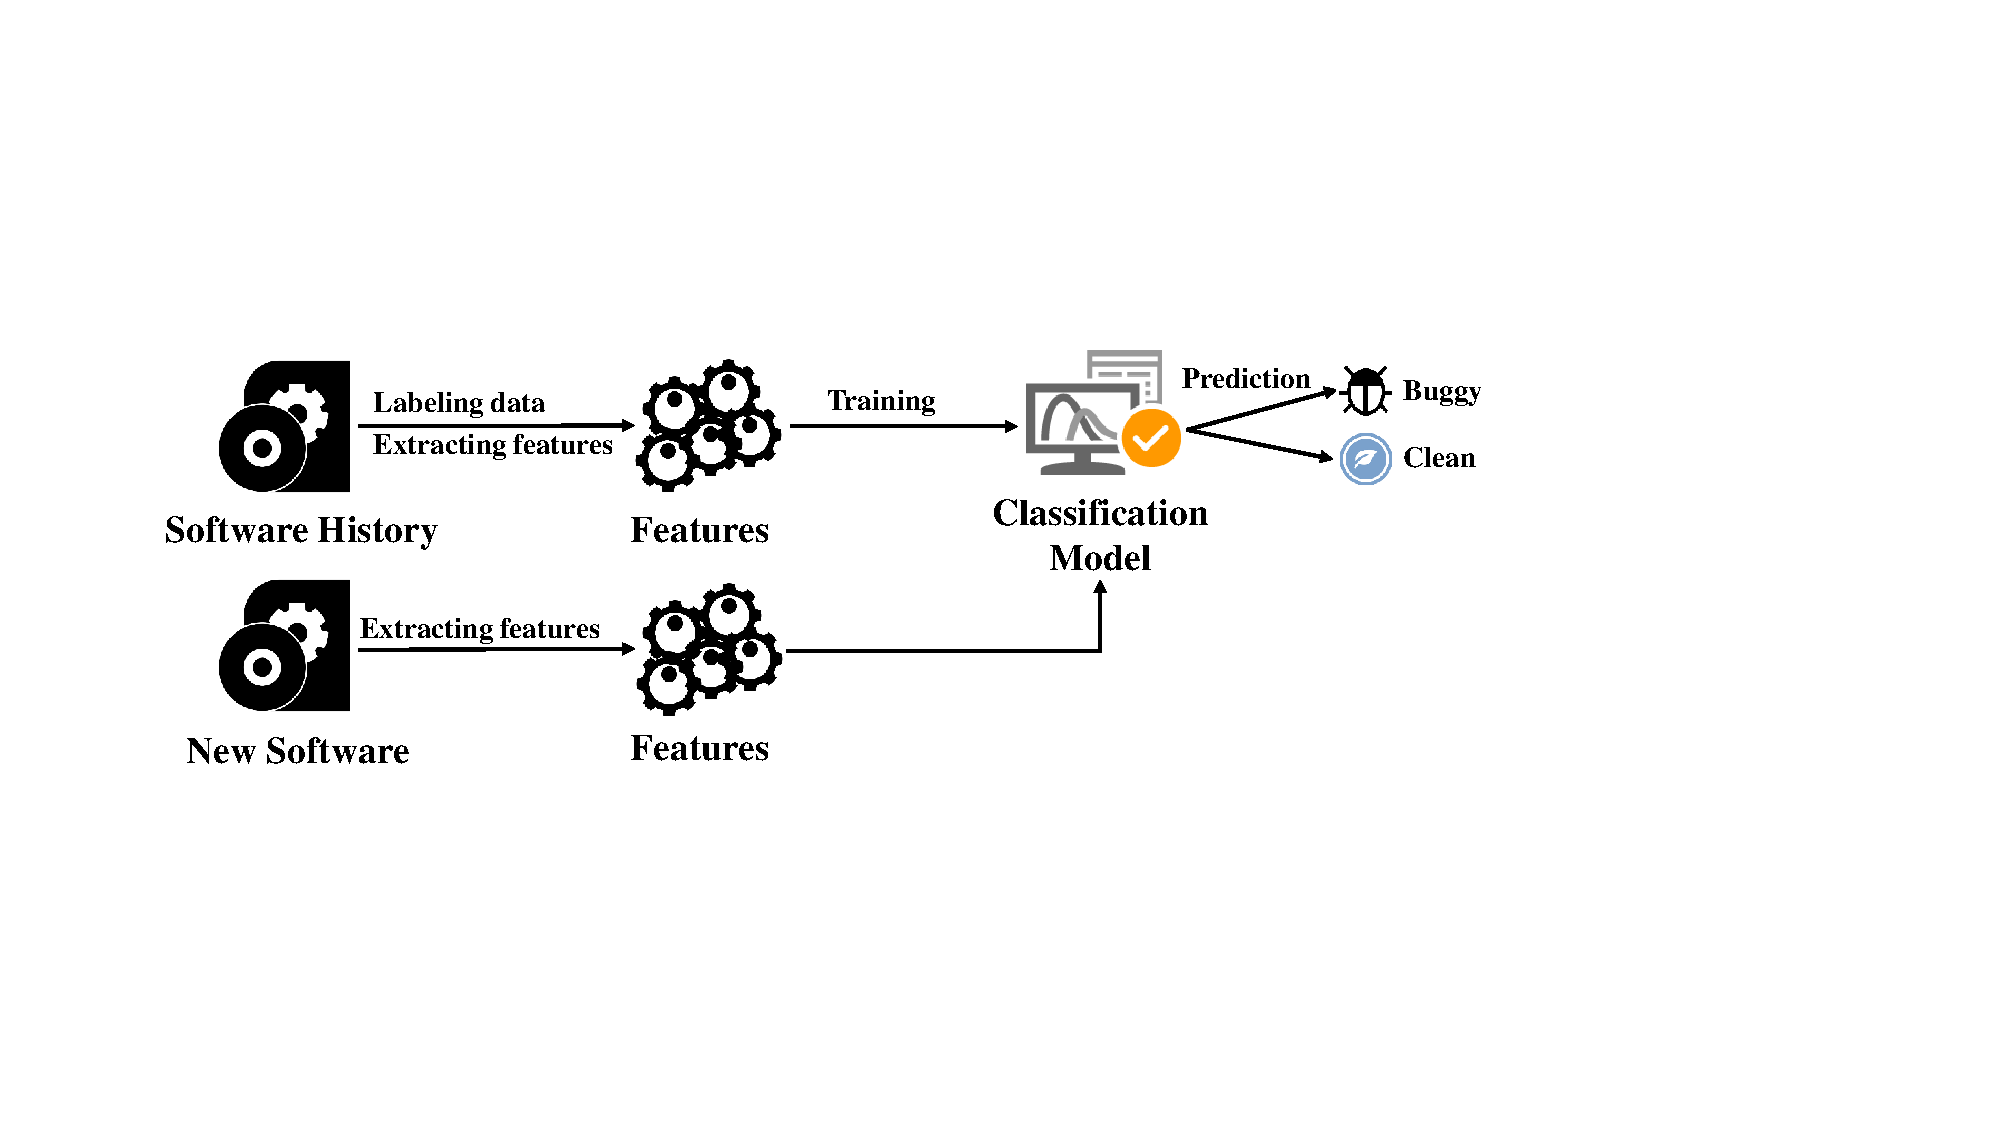
\includegraphics[width=0.85\textwidth]{defect_framework}
%	\caption{Defect Prediction Framework}
%	\label{fig:defect}
%\end{figure*}
\begin{figure}
	\centering
	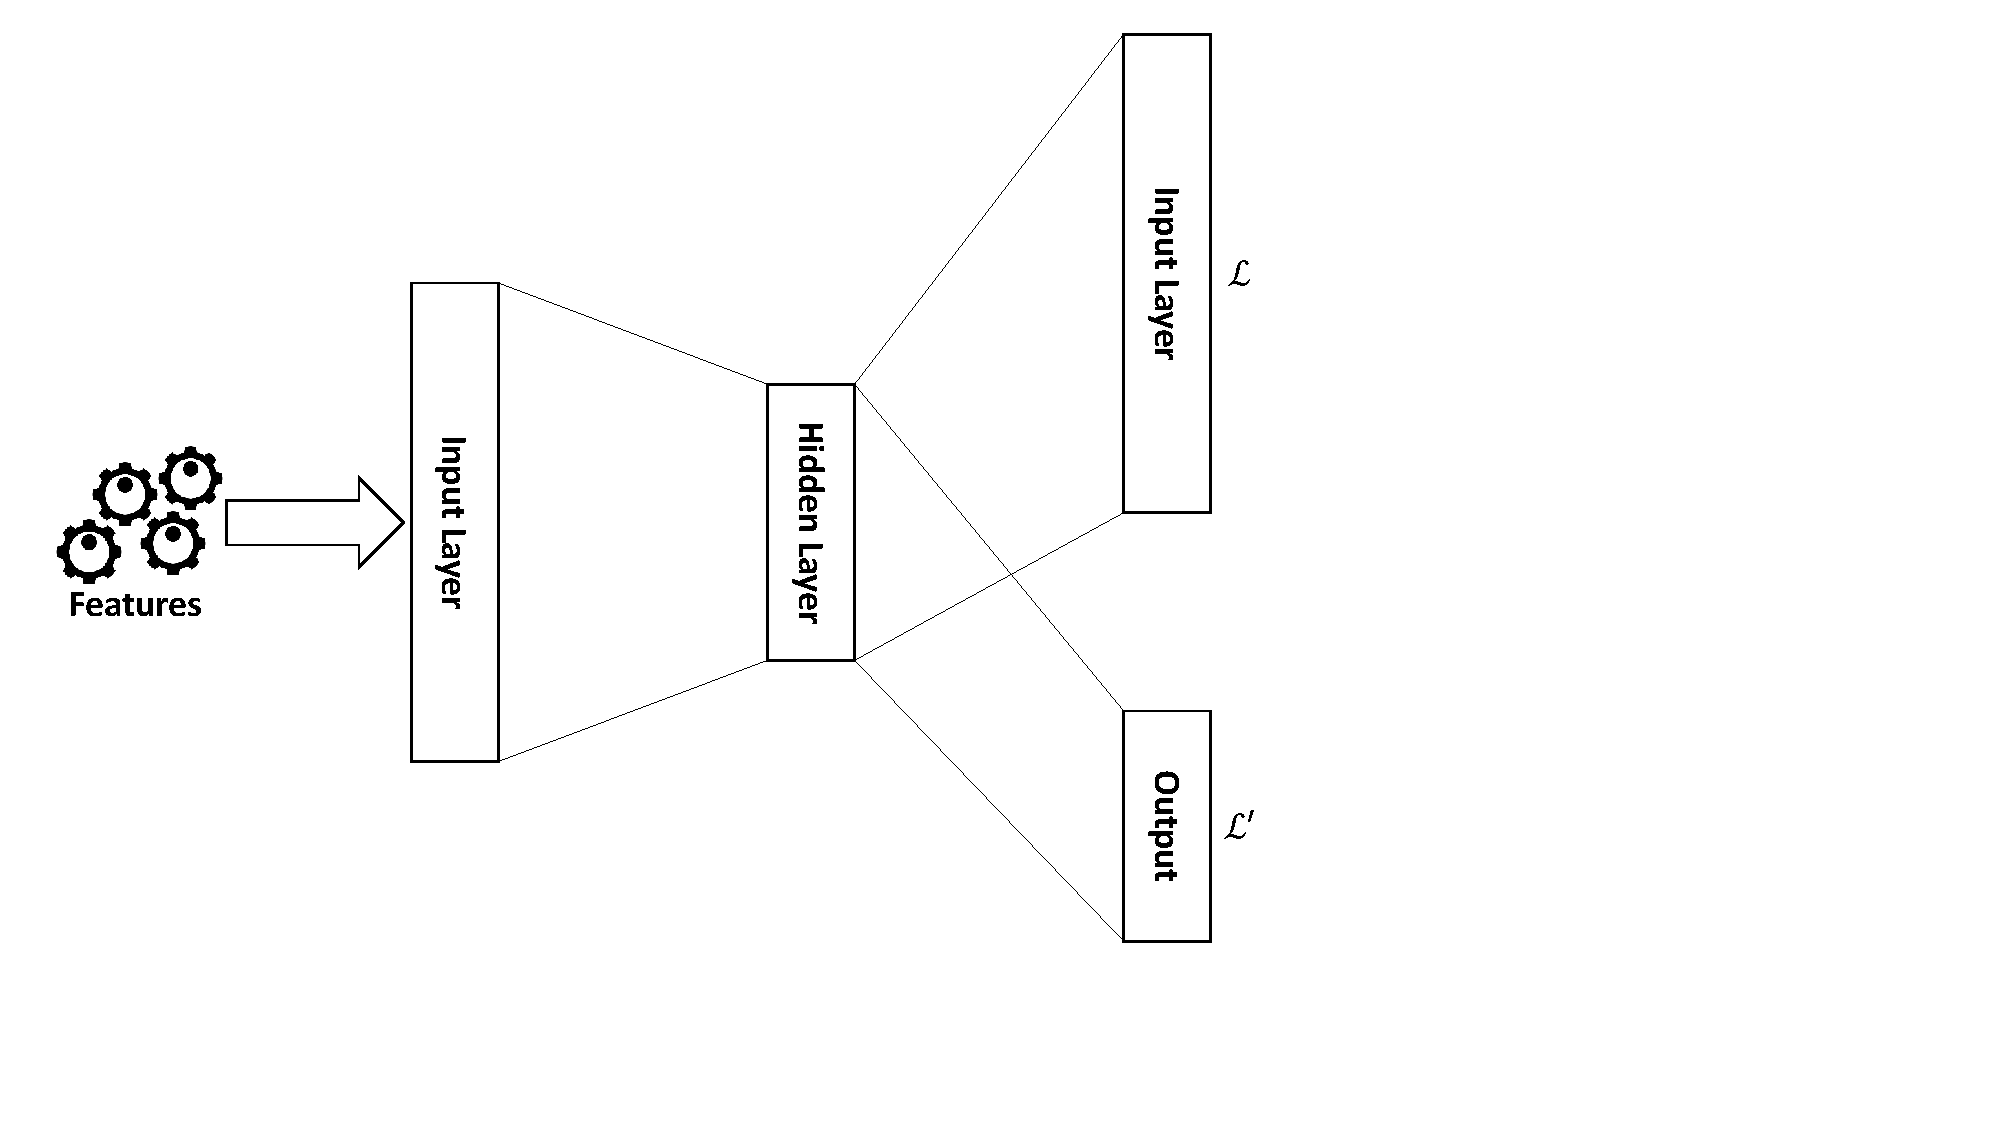
\includegraphics[width=0.45\textwidth]{dssl_framework}
	\caption{Deep Semi-supervised Learning Framework}
	\label{fig:semi_framework}
\end{figure}


%Figure~\ref{fig:defect} presents the overall framework of file-level defect prediction. Typically, the defect prediction problem is solved by following two specific steps. 
The overall process of our file-level defect prediction follows two specific steps. The first step is to label source code files as buggy or clean and then extracts traditional features of these files. These traditional features are introduced in~\cite{wang2016automatically, mccabe1976complexity, chakradeo2013mast}. The second step is to construct a defect prediction model~\cite{bishop2006pattern} to predict whether a new source code file is buggy or clean.  We refer to the software version used for building our defect prediction model as training data and the one used to evaluate the built model as testing data. 

%Figure 2 presents a typical le-level defect prediction process
%that is adopted by existing studies [20,27,34,41,42,51,
%64]. The rst step is to label data as buggy or clean based
%on post-release defects for each le. A le is buggy if the le
%contains bugs. Otherwise, the le is clean. The second step
%is to collect corresponding traditional features of these les.
%Instances with features and labels are used to train machine
%learning classiers. Finally, trained models are used to predict
%new instances as buggy or clean.
%We refer to the set of instances used for building models as
%the training set, whereas the set of instances used to evaluate
%the trained models as the test set. As shown in Figure 2,
%when performing within-project defect prediction (following
%existing work [41], we call this WPDP), the training and test
%sets are from the same project A. When performing crossproject
%defect prediction (following existing work [41] we call
%this CPDP), prediction models are trained by training set
%from a project A (source), and test set is from a dierent
%project B (target).
%In this study, we examine the performance of learned semantic
%features on both WPDP and CPDP.

\subsection{Parsing Source Code and Generating Features}
\label{sec:parsing}
%In our approach, we follow Wang et al.~\cite{wang2016automatically} to extract source code information to learn semantic features. Typically, the syntactic information from source code is collected based on Java Abstract Syntax Tree (AST)~\cite{neamtiu2005understanding}. For each program element, we extract a vector of tokens of the three types of AST nodes: 1) nodes of method invocations and class instance creations, 2) declaration nodes, i.e., method declarations, type declarations, etc. and 3) control-flow nodes such as while statements, catch clauses, if statements, for statements, etc. Note that our semi-supervised learning only takes numerical vectors as inputs, and the lengths of the input vectors are the same. Thus, we apply Wang approaches~\cite{wang2016automatically} to map between integers and tokens, and encode token vectors to integer vector. Note that our integer vectors may have different lengths, we append 0 to the integer vectors to make all the lengths consistent and equal to the length of the longest vector. We also note that adding zeros does not affect the results, since it is simply representation transformation to make the vectors acceptable by neural network~\cite{wang2016automatically}.

In our approach, we follow Wang et al.~\cite{wang2016automatically} approach to extract source code information. Typically, the syntactic information from source code is collected based on Java Abstract Syntax Tree (AST)~\cite{neamtiu2005understanding}. For each Java source code file, we extract a sequence of AST node tokens of these types: 1) nodes of method invocations and class instance creations, 2) declaration nodes, i.e., method declarations, type declarations, and enum declarations, and 3) control-flow nodes such as while statements, catch clauses, if statements, for statements, etc. Unlike Wang approach which encode the extracted tokens as unique integers and use them as features, we encode the tokens using a term frequency - inverse document frequency (TF-IDF)~\cite{manning2008introduction} and consider them as features for our framework (i.e., deep semi-supervised learning). These features reflects how important a token is in its corresponding source code file.

%Note that our semi-supervised learning only takes numerical vectors as inputs, and the lengths of the input vectors are the same. Thus, we apply Wang approaches~\cite{wang2016automatically} to map between integers and tokens, and encode token vectors to integer vector. Note that our integer vectors may have different lengths, we append 0 to the integer vectors to make all the lengths consistent and equal to the length of the longest vector. We also note that adding zeros does not affect the results, since it is simply representation transformation to make the vectors acceptable by neural network~\cite{wang2016automatically}.

%DBN takes only numerical vectors as inputs, and the
%lengths of the input vectors must be the same. To use DBN
%to generate semantic features by using DBN, we rst build
%a mapping between integers and tokens, and encode token
%vectors to integer vectors. Each token has a unique integer
%identier while dierent method names and class names will
%be treated as dierent tokens. Since our integer vectors may
%have dierent lengths, we append 0 to the integer vectors
%to make all the lengths consistent and equal to the length
%of the longest vector. Adding zeros does not aect the
%results, and it is simply a representation transformation to
%make the vectors acceptable by DBN. Taking code snippets
%in Figure 3 as an example, if we consider only \File1" and
%\File2", the token vectors for \File1" and \File2" would be
%mapped to [1, 2, 3, 4] and [2, 3, 1, 4] respectively. Through
%this encoding process, method invocation information and
%inter-class information are represented as integer vectors. In
%addition, some program structure information is preserved
%since the order of tokens remains unchanged.


\subsection{Deep Semi-supervised Learning}
\label{sec:semi}
The goal of defect prediction is to detect source code files that may contain bug in the future. 

Let $\mathcal{X}=\{x_1, x_2, \dots, x_n\}$ denotes the set of source code files in a software project and $\mathcal{Y}=\{y_1, y_2, \dots, y_n\}$ represents the set of labels for the source code files, where $n$ is the number of source code files in the project.  Note that the source code file is labeled as $1$ if it contains bug, otherwise it will be labeled as $0$ which means that it is clean from bug. %The source files can be collected from github repository~\footnote{https://github.com/}
%The source files can be collected from some popular software projects (e.g, ant, camel, lucene, etc.)~\footnote{http://openscience.us/repo/defect/}. 
Unlike traditional approaches~\cite{yang2015deep, wang2016automatically} that independently learn semantic features and construct defect prediction model, our deep semi-supervised learning (DSSL) combines the two tasks for tackling the defect prediction problem. Typically, we attempt to learn a semantic features function $f: \mathcal{X} \longmapsto \mathcal{X}$ and a defect prediction function $f': \mathcal{X} \longmapsto \mathcal{Y}$, $y_i \in \mathcal{Y}=\{0, 1\}$ indicates whether a source code file $x_i \in \mathcal{X}$ contains a bug. % which can be obtained by investigating software commit logs and bug report descriptions~\cite{fischer2003populating}.
These two functions $f$ and $f'$ can be learned by minimizing the following objective function:
%We formalize the our approaches as a joint optimization, expressed by the loss function $\mathcal{L}$, for learning semantic features and building defect prediction model as following:
\begin{equation}
\label{eq:loss}
\begin{split}
\min_{f,f'} \sum_{i}^{}\mathcal{L}(f(x_i), x_i) + \theta \mathcal{L'}(f'(x_i), y_i) \\
+ \lambda \Omega(f, f')
\end{split}
\end{equation}
where $\mathcal{L}(\cdot, \cdot)$ and $\mathcal{L}'(\cdot, \cdot)$ are the empirical loss of the semantic features and the defect prediction functions, respectively. $\theta$ is the predefined value for weighting the two loss functions. $\Omega(f, f')$ is the regularization term imposed on the two functions. The trade-off between the empirical loss and the regularization term is controlled by $\lambda$. 

The overall framework of DSSL is shown in Figure~\ref{fig:semi_framework}. The DSSL model contains three different layers: input layer, hidden layer, and output layer. Given a source code file, the features extracted in Section~\ref{sec:parsing} are fed to the input layer while the corresponding defect label is fed to the output layer. The network consisting of input layer, hidden layer, and input layer represents an encoder-decoder model. The encoder-decoder model is required to learn semantic features. Note that our encoder-decoder model are inspired by autoencoder~\cite{ng2011sparse}, which is an unsupervised learning technique. The original autoencoder only learn the function $f: \mathcal{X} \longmapsto \mathcal{X}$ so that the output values $\mathcal{\hat{X}}$ are similar to input values $\mathcal{X}$. On the other hand, DSSL attempts to learn semantic features and optimize defect prediction task, thus it takes into account two functions, i.e., $f$ and $f'$, which represents the semantic features and defect prediction function, respectively. $f'$ is learned through the connection between the hidden layer and the output layer. According to Figure~\ref{fig:semi_framework}, our model optimizes two loss functions, i.e., $\mathcal{L}$ and $\mathcal{L'}$ to construct the defect prediction model. In encoder-decoder model, we employ a fully connected neural network for learning to convert low level features from source code files to semantic features. At the same time, our network learns to determine on whether the given source code file is buggy based on the semantic features. 

%The overall framework of DSSL is shown in Figure~\ref{fig:semi_framework}. The DSSL model contains two four different parts: parsing abstract syntax tree, generating features, encoder, and decoder. The first two steps are briefly described in Section~\ref{sec:parsing} to feed source files data to our deep neural network. Encoder and decoder are required to learn semantic features as well as defect prediction model. Note that our encoder and decoder steps are inspired by autoencoder~\cite{ng2011sparse} which is an unsupervised learning technique. However the original autoencoder only tries to learn the function $f: \mathcal{X} \longmapsto \mathcal{X}$ so that the output values $\mathcal{\hat{X}}$ are similar to input values $\mathcal{X}$. However, SSA attempts to learn semantic features and optimize defect prediction model, thus it takes into account of two functions, i.e., $f$ and $f'$ represent the semantic features and defect prediction respectively. According to Figure~\ref{fig:semi_framework}, our model tries to optimize two different loss functions, i.e., $\mathcal{L}$ and $\mathcal{L'}$ to construct the defect prediction model. In encoder and decoder steps, we employ a fully connected neural network to fuse middle-level features extracted from source files to generate semantic features, where our network is learn to facilitate the determination on whether the given source code file is related to the given bug report based on the semantic features. In this paper, we employ Adam optimization~\cite{kingma2014adam}, which is popular optimization method in deep learning community, to optimize the two loss functions for constructing defect prediction model. 

%In the cross-language feature fusion layers, we employ a fully connected neural network to fuse middle-level features ex- tracted from bug reports and source files to generate a unified feature representation, where the network is learned in order to facilitate the determination on whether the given source code file is related to the given bug report based on the uni- fied feature.


%To learn semantic features from program elements, we employ autoencdoer

%Ω(f) is a regulariza- tion term imposing on the prediction function. The trade-off between L(·, ·) and Ω(f ) is balanced by λ.

%Let C = fc1; c2;    ; cN1g denotes the set of source code
%files of a software project andR = fr1; r2;    ; rN2g denotes
%the collection of bug reports received by the software maintenance
%team, where N1;N2 are the number of source files and
%bug reports, respectively. The bug reports and source files can
%be collected from bug tracking systems (e.g., Bugzilla, Jira,
%etc.) and history control systems (e.g., CVS, Git, etc.).

\subsection{Imbalanced Problem in Defect Prediction}
\label{sec:imbalanced}
In defect prediction tasks, often times there are only a few source code files that contain bugs while the other source code files are \textit{clean}~\cite{khoshgoftaar2010attribute}. This consequently makes the labeled data to be imbalanced. This imbalanced nature increases the learning difficulty. For this reason, imbalanced class learning, which specializes in tackling classification problems involving imbalanced data, is helpful for defect prediction problem~\cite{wang2013using}. To address this imbalanced data issue, we propose a balanced random sampling procedure when picking a data instance to update our DSSL network weights. In particular, we select a random instance from each the positive and negative instance pools to mitigate the issue of skewed distribution. This mitigates the issue of imbalanced data in defect prediction. 


%To address this problem, we propose to learn the semantic features that may counteract the negative influence of the imbalanced data in the subsequent learning of defect prediction function. Inspired by~\cite{zhou2006training}, we introduce an unequal misclassification cost according to the imbalance ratio and train the fully connected network in a cost-sensitive manner. 
%
%Let $r_n$ denote the ratio cost of incorrectly associating an \textit{clean} source code file to a bug program element and $r_p$ denote the cost of missing a buggy source code file in the training data. The weight of the semi-supervised autoencoder (SSA) networks $\mathcal{W}$  can be learned by minimizing the following objective function following Adam optimization~\cite{kingma2014adam}. 
%\begin{equation}
%\label{eq:imbalanced}
%\begin{split}
%\min_{\mathcal{W}} \sum_{i}^{}\mathcal{L}(f(x_i), x_i) 
%+ r_n \mathcal{L}'(x_i, y_i;\mathcal{W}) y_i \\ + r_p \mathcal{L}'(x_i, y_i;\mathcal{W}) (1 - y_i) + \lambda \rVert \mathcal{W} \rVert^2
%\end{split}
%\end{equation}
%where $\mathcal{L}$ and $\mathcal{L}'$ are the loss function for semantic features and defect prediction model, respectively. $\lambda$ is the trade-off parameter.  
%To address this, we devise a balanced random
%sampling procedure when picking a data instance for gradient
%descent update. In particular, for every update step, we
%alternatingly select a random instance from the positive and
%negative instance pools, as per lines 4-8 of Algorithm 1.
%Using this simple method, we can balance the training
%from positive and negative instances, thus effectively mitigating
%the issue of skewed distribution in the localization
%task. It is also worth noting that our iterative tuning procedure
%is efficient. That is, its time complexity is linear with
%respect to the number of instances N and maximum iterations
%Tmax.


%Let costn denote the cost of incorrectly associating an ir- relevant source code file to a bug report and costp denote the cost of missing a buggy source code file that is responsible for the reported bugs. The weight of the fully connected net- works w can be learned by minimizing the following objec- tive function based on SGD (stochastic gradient descent).

%the imbalanced nature of this type of data increases the learning difficulty of such a task. Class imbalance learning specializes in tackling classification problems with imbalanced distributions, which could be helpful for defect prediction, but has not been investigated in depth so far. In this paper, we study the issue of if and how class imbalance learning methods can benefit software defect prediction with the aim of finding better solutions.    



%In the cross-language feature fusion layers, we employ a fully connected neural network to fuse middle-level features ex- tracted from bug reports and source files to generate a unified feature representation, where the network is learned in order to facilitate the determination on whether the given source code file is related to the given bug report based on the uni- fied feature.
%In most cases of bug localization, a reported bug may be only related to one or only a few source code files, while a large number of source code files are irrelevant to the given bug report. Such an imbalance nature increases the difficulty in learning a well-performing prediction function based on the unified feature.
%To address this problem, we propose to learn the unified feature that may counteract the negative influence of the im- balanced data in the subsequent learning of prediction func- tion. Inspired by [Zhou and Liu, 2006], we introduce an un- equal misclassification cost according to the imbalance ratio and train the fully connected network in a cost-sensitive man- ner.
%Let costn denote the cost of incorrectly associating an ir- relevant source code file to a bug report and costp denote the cost of missing a buggy source code file that is responsible for the reported bugs. The weight of the fully connected net- works w can be learned by minimizing the following objec- tive function based on SGD (stochastic gradient descent).

\subsection{Setting for Training Deep Semi-supervised Learning}
\label{sec:setting}
In our setting, the number of hidden layers, the number of nodes in each hidden layer, the number of iterations, and $\theta$ are chosen by performing cross validation on training data. By default, the number of hidden layers, the number of nodes in each hidden layer, and number of iteration are selected as 2, 1000-100, and 75, respectively. We employ Adam optimization~\cite{kingma2014adam}, which is popular optimization method in deep learning community, to optimize the two loss functions for constructing DSSL. %Note that $\theta$ in Equation~\ref{eq:loss} is also well-chosen based on training data to solving imbalanced between two loss functions. 


%Some deep learning application~\cite{hinton2009deep, ng2011sparse} reports an effective of deep learning models need well-tuned parameters, i.e., 1) the number of hidden layers, 2) the number of nodes in each hidden layer, and 3) the number of iterations.
%In our deep semi-supervised learning, we choose two hidden layers and  these parameters are chosen by learning from training data 
%
% In~\cite{wang2016automatically}, the authors pointed out that the deep learning model was optimized when they chose 10, 100, 200 as the number of hidden layers, number of nodes in each hidden layer, and number of iterations respectively. For the fair comparison with~\cite{wang2016automatically}, we use these parameters to train our deep semi-supervised learning model. 

%Many DBN applications [6,25,37] report that an eective
%DBN needs well-tuned parameters, i.e., 1) the number of hid-
%den layers, 2) the number of nodes in each hidden layer, and
%3) the number of iterations. In this study, since we leverage
%DBN to generate semantic features, we need to consider the
%impact of the three parameters. We tune the three parameters
%by conducting experiments with dierent values of the
%parameters on ant (1.5, 1.6), camel (1.2, 1.4), jEdit (4.0,
%4.1), lucene (2.0, 2.2), and poi (1.5, 2.5) respectively. Each
%experiment has specic values of the three parameters and
%runs on the ve projects individually. Given an experiment,
%for each project, we use the older version of this project to
%train a DBN with respect to the specic values of the three
%parameters. Then, we use the trained DBN to generate semantic
%features for both the older and newer versions. After
%that, we use the older version to build a defect prediction
%model and apply it to the newer version. Lastly, we evaluate
%the specic values of the parameters by the average F1 score
%of the ve projects in defect prediction.





\section{Experimental Results}
\label{sec:exp_results}
We conduct extensive experiments to study the performance of the proposed approach and compare it with existing defect prediction approaches. We also discuss threats to the validity of our approach.

\subsection{Evaluation Metrics}
\label{sec:metrics}
To measure defect prediction results, we employ three different metrics: \textit{Precision}, \textit{Recall} and \textit{F1}. These evaluation metrics are widely used to evaluate the performance of defect prediction~\cite{menzies2007data, menzies2010defect, nam2013transfer} as well as information retrieval binary classification~\cite{manning2008introduction}. Typically, precision is the fraction of retrieved instances that are relevant, recall is the fraction of relevant instances that are retrieved, whereas F1 combines both precision and recall to measure the performance of our model. Below is the equation of these metrics:
\begin{equation}
\label{eq:precision}
Precision = \frac{TP}{TP+FP}
\end{equation}

\begin{equation}
\label{eq:recall}
Recall = \frac{TP}{TP+FN}
\end{equation}

\begin{equation}
\label{eq:f1}
F1 = \frac{2 * Precision * Recall}{Precision + Recall}
\end{equation}
where \textit{TP}, \textit{FP}, and \textit{FN} are considered as true positive, false positive, and false negative respectively. True positive is the number of predicted defective files that are truly defective, while false positive is the number of predicted defective files that are actually not defective. False negative records the number of predicted non-defective files that are actually defective. A higher precision makes the manual inspection on a certain amount of predicted defective files find more defects, while an increase in recall can reveal more defects given a project. F1 takes consideration of both precision and recall.


\subsection{Datasets}
\label{sec:dataset}

\textcolor{red}{Ferdian: Can you help me to rewrite dataset section?}

We perform several steps to create our benchmark dataset. Firstly, we fetch top 2,500 most popular open-source Java projects from GitHub (sorted by the sum of their number of stars and number of forks). GitHub contains many toy projects, thus, we only consider popular projects similar to prior studies~\cite{ray2014large, kochhar2016large}. We only clone the git repositories of projects which use Maven as we leverage Maven to automatically build the projects and construct call graphs from compiled classes. Out of the 2500 projects, 831 projects use Maven. Secondly, we collect 342 Apache Java projects which use Maven and are hosted on GitHub. A er removing the overlapping projects, our dataset contains 1,143 projects.

Next, we ignore projects with less than 150 source files as these projects are too small to employ deep neural netwok. We also  filter out projects which have less than 100 tested files. For each project, we have two versions: current version (i.e., latest version as of June 2016) which serves as a test dataset, and previous version (i.e., version one year prior to current version) which serves as a training set. We compile these two versions using \textit{mvn compile:compile}. We ignore projects whose current and/or previous version cannot be compiled. In the end, our dataset has 28 projects.

Table~\ref{tab:data} shows the overview of our dataset containing 28 projects. In average, our data has around 921 source files in training set and more than 1020 program elements in testing set. Average bug rate is 18.7\% and 7.5\% on training and testing data respectively showing the imbalanced problem in defect prediction~\cite{wang2013using, khoshgoftaar2010attribute}. 

%having a total of 46 million SLOC, 83 thousand source code  les, 0.9 million methods, 280 thousand commits and over 45 thousand test  les contributed by more than 5 thousand developers spanning over period of 15 years, i.e., 2001-2016. Our dataset con- tains popular projects such as Apache Commons IO [4], which is a library of utilities for IO functionalities and Joda-Time [31], which is date and time library for Java.

\subsection{Baselines}
\label{sec:baselines}
%To evaluate the performance of our approach in defect prediction, we compare with traditional features (see Section~\ref{sec:relatedwork}). The first baseline consists some traditional features, including lines of code, cyclomatic complexity~\cite{mccabe1976complexity}, total number of methods, total number of public methods, total number of local methods, the depth of inheritance tree, comment density, etc. These features are well described in~\cite{hassan2009predicting} and have been widely used in previous work~\cite{jing2014dictionary, menzies2007data, menzies2010defect, nam2013transfer, zimmermann2007predicting, yang2015deep}. Since they are popular features so we can directly compare our work with previous studies. We note that the traditional features do not contain Abstract Syntax Tree (AST) nodes, which are described in this paper. 

We compare our approach with the defect prediction models constructed based on two traditional features. The first traditional features are embedding features generated following Wang et al.~\cite{wang2016automatically}. The second traditional features are AST features extracted from source code's AST. Specifically, we collect AST nodes from source code and represent the source code as a vector of term frequencies of the AST nodes. These two baselines were shown their effectiveness in solving defect prediction problem~\cite{wang2016automatically}.

%To evaluate the performance of our approach in defect prediction, we compare it with traditional defect prediction models that are constructed using the state-of-the-art semantic features learning approach by Wang et al.~\cite{wang2016automatically}. They employ Deep Belief Network~\cite{hinton2009deep} to automatically learn semantic features from token vectors extracted from source code's AST. They have shown that their semantic features significantly improve the performance of defect prediction. 

%The second baseline includes semantic features constructed following Wang et al. approaches~\cite{wang2016automatically}. Typically, they tried to employ deep belief network~\cite{hinton2009deep} to automatically learn semantic features from token vectors extracted from programs' AST. They also proved that their semantic features significantly improve the performance of defect prediction in software engineering domain. 

We employ three popular machine learning algorithms~\cite{bishop2006pattern} to build defect prediction models for each traditional features. These algorithms are widely used in software engineering~\cite{wang2016automatically, wang2013using, jing2014dictionary} described as follows: 
\begin{itemize}
%	\item Decision tree is used to build a tree-based predictive model where branch nodes represent an option on feature values while leaf nodes represent predicted values. Tree models in which the predicted values are taken from a finite set are called classification trees. In these tree structures, leaf nodes represent class labels and branch node sequences represent conjunctions of features that lead to those class labels. This algorithm is very popular in statistics, data mining and machine learning~\cite{safavian1991survey}.
	\item Decision tree is used to build a tree-based classification model where branch nodes represent an option on feature values while leaf nodes represent predicted values~\cite{safavian1991survey}.
%	\item Logistic regression is a predictive model that explains the relationship between one dependent binary variable and one or more nominal, ordinal, interval or ratio-level independent variables. Logistic regression is used in various applications like: health, statistics, data analysis, etc.~\cite{hosmer2013applied}.
	\item Logistic regression is a well-known classification model that employs in various application such as: health, statistics, data analysis, etc.~\cite{hosmer2013applied}. 
%	explains the relationship between one dependent binary variable and one or more nominal, ordinal, interval or ratio-level independent variables. Logistic regression is used in various applications like: health, statistics, data analysis, etc.~\cite{hosmer2013applied}.
	\item Na\"{i}ve Bayes classifier, which are highly scalable, is a simple probabilistic classifiers based on applying Bayes' theorem ~\cite{vapnik1998statistical}. 
%	with strong (naive) independence assumptions between the features. Naive Bayes classifiers are highly scalable, requiring only a number of parameters that is linear with the number of variables (features/predictors). For some types of probability models, Naive Bayes classifiers can be trained very efficiently in a supervised learning setting. In many practical applications, parameter estimation for Naive Bayes models uses the method of maximum likelihood~\cite{pan2002maximum}.
\end{itemize}

%The 20 traditional features are available for PROMISE data, and the work from He et al. [13] contains the full list of the 20 features, which are well described in their Table II. These features and data have been widely used in previous work [20, 33, 34, 42, 70]. We choose the widely used PROMISE data so that we can directly com- pare our work with previous studies. Note that, for a fair comparison, we also perform the noise removal approach de- scribed in Section 3.2.1 on the PROMISE data.


%The traditional features from PROMISE do not contain AST nodes, which were used by our DBN models. For a fair comparison, our second baseline of traditional features is the AST nodes that were given to our DBN models, i.e., the AST nodes in all files after fixing noise (Section 3.2.1). Each instance is represented as a vector of term frequencies of the AST nodes.

%To bridge the gap between programs' semantics and
%defect prediction features, this paper proposes to leverage a
%powerful representation-learning algorithm, deep learning,
%to learn semantic representation of programs automatically
%from source code. Specically, we leverage Deep Belief
%Network (DBN) to automatically learn semantic features
%from token vectors extracted from programs' Abstract
%Syntax Trees (ASTs).
%Our evaluation on ten open source projects shows that
%our automatically learned semantic features signicantly improve
%both within-project defect prediction (WPDP) and
%cross-project defect prediction (CPDP) compared to traditional
%features. Our semantic features improve WPDP on
%average by 14.7% in precision, 11.5% in recall, and 14.2%
%in F1. For CPDP, our semantic features based approach
%outperforms the state-of-the-art technique TCA+ with traditional
%features by 8.9% in F1.

% Table generated by Excel2LaTeX from sheet 'WithinProjects'
\begin{table*}[t!]
	\centering
	\caption{
%		Comparison between DDA and three classification algorithms (decision tree, logistic regression, and na\"{i}ve Bayes) using semantic features and AST features. P, R, and F1 denote precision, recall and F1 score respectively and are measured by percentage. The best F1 scores are highlighted in bold.
		Precision, recall and F1 scores of within-project prediction. All the scores are measured by percentage. The best F1 scores are highlighted in bold. Deep discriminative autoencoder, decision tree, logistic regression, and na\"{i}ve Bayes are denoted as DDA, DT, LR, NB respectively. 
	}
	\begin{adjustbox}{width=1\textwidth}
	\begin{tabular}{|c|c|c|c|c|c|c|c|}
		\hline
		\multirow{3}[6]{*}{Project} & \multirow{2}[4]{*}{DDA} & \multicolumn{3}{c|}{Embedding} & \multicolumn{3}{c|}{AST} \\
		\cline{3-8}          &       & DT    & LR    & NB    & DT    & LR    & NB \\
		\cline{2-8}          & P R F1 & P R F1 & P R F1 & P R F1 & P R F1 & P R F1 & P R F1 \\
		\hline
		\hline
		\multicolumn{1}{|l|}{Checkstyle} & 74.6 84.7 \textbf{79.3} & 78.3 55.3 64.8 & 83.6 68.8 75.5 & 72.3 82.9 77.3 & 82.4 63.5 71.8 & 79.7 62.4 70.0  & 82.7 64.7 72.6 \\

		\multicolumn{1}{|l|}{Nuvolabase} & 33.8 66.0 \textbf{44.7} & 32.8 7.51 12.2 & 36.2 44.7 40.0 & 31.1 73.5 43.7 & 50.7 14.2 22.2 & 59.6 12.2 20.3  & 20.3 41.1 27.1 \\
		
		\multicolumn{1}{|l|}{OrientDB} & 32.9 47.9 \textbf{39.0} & 25.6 6.94 10.9 & 27.3 47.2 34.6 & 20.8 69.4 32.0 & 40.3 18.8 25.6 & 44.2 13.2 20.3  & 12.1 38.2 18.4 \\
		
		\multicolumn{1}{|l|}{Traccar} & 33.9 75.0 \textbf{46.7} & 14.0 80.0 23.9 & 12.7 75.0 21.7 & 12.8 95.0 22.0 & 20.0 20.0 20.0 & 12.2 70.0 20.7  & 9.47 90.0 17.1 \\
		\hline
		\hline
		Average & 43.8 68.4 \textbf{52.4} & 37.7 37.4 28.0 & 39.9 58.9 42.9 & 34.3 80.2 43.8 & 48.4 29.1 34.9 & 48.9 39.5 32.8 & 31.1 58.5 33.8 \\
		\hline
	\end{tabular}%
	\end{adjustbox}
	\label{tab:within}%
\end{table*}%


% Table generated by Excel2LaTeX from sheet 'CrossProjects'
\begin{table}[t!]
	\centering
	\caption{Precision, recall and F1 scores of cross-project defect prediction. All the scores are measured by percentage. The best F1 scores are highlighted in bold.}
	\begin{adjustbox}{width=0.48\textwidth}
	\begin{tabular}{|c|c|c|c|c|}
		\hline
		\multirow{3}[6]{*}{Source } & \multirow{3}[6]{*}{Target} & \multicolumn{2}{c|}{Cross-project} & \multirow{2}[4]{*}{Within-project} \\
		\cline{3-4}          &       & DDA & Embedding &  \\
		\cline{3-5}          &       & P R F1 & P R F1 & P R F1 \\
		\hline
		\hline
		\multicolumn{1}{|l|}{Nuvolabase} & \multicolumn{1}{l|}{Checkstyle} & 79.0 57.6 \textbf{66.7} & 54.5 38.8 45.3  & \multirow{2}[4]{*}{74.6 84.7 79.3} \\
		\cline{1-4}    \multicolumn{1}{|l|}{OrientDB} & \multicolumn{1}{l|}{Checkstyle} & 94.3 29.4 44.8 & 54.7 48.2 \textbf{51.3} &  \\
		\hline
		\multicolumn{1}{|l|}{Checkstyle} & \multicolumn{1}{l|}{Nuvolabase} & 45.5 36.4\textbf{ 40.4} & 27.0 52.2 35.6 & \multirow{2}[4]{*}{33.8 66.0 44.7} \\		
		\cline{1-4}    \multicolumn{1}{|l|}{Traccar} & \multicolumn{1}{l|}{Nuvolabase} & 44.2 36.4 \textbf{40.0} & 27.1 41.5 32.8 &  \\
		\hline
		\multicolumn{1}{|l|}{Nuvolabase} & \multicolumn{1}{l|}{OrientDB} & 57.1 16.7\textbf{ 25.8}  & 16.2 31.9 21.5 & \multirow{2}[4]{*}{32.9 47.9 39.0} \\
		\cline{1-4}    \multicolumn{1}{|l|}{Traccar} & \multicolumn{1}{l|}{OrientDB} & 25.4 43.1 \textbf{31.9} & 18.5 45.1 26.3 &  \\
		\hline
		\multicolumn{1}{|l|}{Nuvolabase} & \multicolumn{1}{l|}{Traccar} & 13.9 85.0 \textbf{23.9} & 16.7 15.0 15.8 & \multirow{2}[4]{*}{33.9 75.0 46.7} \\
		\cline{1-4}    \multicolumn{1}{|l|}{Checkstyle} & \multicolumn{1}{l|}{Traccar} & 16.0 20.0 \textbf{17.8} & 9.80 50.0 16.4 &  \\
		\hline
		\hline
		\multicolumn{2}{|c|}{Average} & 46.9 40.6 \textbf{36.4} & 28.1 40.3 30.6 & 43.8 68.4 52.4 \\
		\hline
	\end{tabular}%
	\end{adjustbox}
	\label{tab:cross}%
\end{table}%

\begin{table}[t!]
	\centering
	\caption{Training time of the proposed DDA approach}
	\begin{tabular}{|l|c|}
		\hline
		\multicolumn{1}{|c|}{Project} & Time (s) \\
		\hline
		\hline
		Checkstyle & 10.2 \\
		Nuvolabase & 62.5 \\
		OrientDB & 59.2 \\
		Traccar & 5.67 \\
		\hline
		\hline 
		Average & 34.4 \\
		\hline 
	\end{tabular}%
	\label{tab:time}%
\end{table}%


%\begin{table*}[t!]
%	\centering
%	\caption{Data descriptions}
%	\begin{tabular}{|l|c|c|c|c|}
%		\hline
%		\multirow{2}[4]{*}{Project} & \multicolumn{2}{c|}{Number of source files} & \multicolumn{2}{c|}{Average bug rate} \\
%		\cline{2-5}          & Training & Testing & Training & Testing \\
%		\hline
%		\hline
%		alibaba\_druid & 446   & 505   & 0.078 & 0.024 \\
%		apache\_calcite & 1555  & 1981  & 0.177 & 0.051 \\
%		apache\_commons-math & 712   & 742   & 0.056 & 0.038 \\
%		apache\_ignite & 684   & 1204  & 0.016 & 0.068 \\
%		apache\_jackrabbit-oak & 762   & 840   & 0.151 & 0.056 \\
%		apache\_jclouds & 910   & 972   & 0.184 & 0.087 \\
%		apache\_kylin & 623   & 669   & 0.061 & 0.142 \\
%		apache\_olingo-odata2 & 1285  & 1290  & 0.040 & 0.019 \\
%		apache\_phoenix & 1378  & 1408  & 0.139 & 0.042 \\
%		apache\_qpid-java & 551   & 504   & 0.069 & 0.048 \\
%		apache\_qpid-jms & 834   & 881   & 0.174 & 0.102 \\
%		apache\_struts & 1429  & 1485  & 0.186 & 0.120 \\
%		apache\_syncope & 327   & 488   & 0.070 & 0.115 \\
%		apache\_tika & 1321  & 1209  & 0.011 & 0.016 \\
%		BaseXdb\_basex & 825   & 902   & 0.975 & 0.092 \\
%		checkstyle\_checkstyle & 2234  & 2428  & 0.038 & 0.061 \\
%		eclipse\_jgit & 487   & 493   & 0.109 & 0.028 \\
%		haraldk\_TwelveMonkeys & 2234  & 2428  & 0.038 & 0.061 \\
%		izpack\_izpack & 1430  & 944   & 0.326 & 0.097 \\
%		jclouds\_jclouds & 918   & 1243  & 0.231 & 0.092 \\
%		liquibase\_liquibase & 200   & 216   & 0.220 & 0.074 \\
%		metamx\_druid & 551   & 504   & 0.069 & 0.048 \\
%		nutzam\_nutz & 274   & 663   & 0.730 & 0.080 \\
%		openmicroscopy\_bioformats & 1014  & 1227  & 0.118 & 0.029 \\
%		spring-projects\_spring-roo & 738   & 727   & 0.060 & 0.067 \\
%		SpringSource\_spring-roo & 590   & 753   & 0.775 & 0.259 \\
%		torodb\_torodb & 1079  & 1506  & 0.117 & 0.069 \\
%		WindowsAzure\_azure-sdk-for-java & 400   & 424   & 0.030 & 0.116 \\
%		\hline
%		\hline
%		\textbf{Average} & 921.107 & 1022.714 & 0.187 & 0.075 \\
%		\hline
%	\end{tabular}%
%	\label{tab:data}%
%\end{table*}%
%
%

%
%% Table generated by Excel2LaTeX from sheet 'DT'
%\begin{table*}[t!]
%	\centering
%	\caption{Comparison between our approaches vs. two baselines of different features (traditional features and semantic features) using decision tree. P, R, and F1 denote precision, recall, and F1 score respectively. The average F1 scores are highlighted in bold.}
%	\begin{tabular}{|l|ccc|ccc|ccc|}
%		\hline
%		\multirow{2}[4]{*}{Project} & \multicolumn{3}{c|}{Code features} & \multicolumn{3}{c|}{Semantic features} & \multicolumn{3}{c|}{SSA} \\
%		\cline{2-10}          & P     & R     & F1    & P     & R     & F1    & P     & R     & F1 \\
%		\hline
%		\hline
%		alibaba\_druid & 0.352 & 0.951 & 0.514 & 0.694 & 0.051 & 0.096 & 0.372 & 0.083 & 0.136 \\
%		apache\_calcite & 0.561 & 0.385 & 0.457 & 0.457 & 0.071 & 0.124 & 0.466 & 0.667 & 0.549 \\
%		apache\_commons-math & 0.836 & 0.351 & 0.494 & 0.426 & 0.388 & 0.406 & 0.401 & 0.393 & 0.397 \\
%		apache\_ignite & 0.428 & 0.382 & 0.404 & 0.426 & 0.400 & 0.413 & 0.511 & 0.598 & 0.551 \\
%		apache\_jackrabbit-oak & 0.381 & 0.239 & 0.294 & 0.432 & 0.036 & 0.066 & 0.466 & 0.681 & 0.553 \\
%		apache\_jclouds & 0.424 & 0.075 & 0.127 & 0.392 & 0.061 & 0.106 & 0.509 & 0.706 & 0.591 \\
%		apache\_kylin & 0.590 & 0.799 & 0.679 & 0.501 & 0.359 & 0.418 & 0.585 & 0.589 & 0.587 \\
%		apache\_olingo-odata2 & 0.485 & 0.407 & 0.443 & 0.466 & 0.438 & 0.451 & 0.414 & 0.560 & 0.476 \\
%		apache\_phoenix & 0.444 & 0.310 & 0.365 & 0.327 & 0.528 & 0.404 & 0.410 & 0.559 & 0.473 \\
%		apache\_qpid-java & 0.403 & 0.225 & 0.289 & 0.417 & 0.327 & 0.367 & 0.422 & 0.625 & 0.504 \\
%		apache\_qpid-jms & 0.462 & 0.343 & 0.393 & 0.299 & 1.000 & 0.460 & 0.468 & 0.689 & 0.558 \\
%		apache\_struts & 0.316 & 0.043 & 0.076 & 0.326 & 0.280 & 0.302 & 0.547 & 0.713 & 0.619 \\
%		apache\_syncope & 0.323 & 0.012 & 0.024 & 0.622 & 0.589 & 0.605 & 0.501 & 0.393 & 0.441 \\
%		apache\_tika & 0.405 & 0.308 & 0.350 & 0.374 & 0.525 & 0.437 & 0.409 & 0.474 & 0.439 \\
%		BaseXdb\_basex & 0.534 & 0.248 & 0.339 & 0.573 & 0.878 & 0.694 & 0.462 & 0.964 & 0.625 \\
%		checkstyle\_checkstyle & 0.445 & 0.814 & 0.575 & 0.251 & 0.211 & 0.229 & 0.459 & 0.476 & 0.467 \\
%		eclipse\_jgit & 0.455 & 0.364 & 0.404 & 0.396 & 0.857 & 0.542 & 0.417 & 0.429 & 0.422 \\
%		haraldk\_TwelveMonkeys & 0.484 & 0.510 & 0.497 & 1.000 & 0.517 & 0.682 & 0.440 & 0.476 & 0.457 \\
%		izpack\_izpack & 0.266 & 0.561 & 0.361 & 0.541 & 0.714 & 0.616 & 0.485 & 0.576 & 0.527 \\
%		jclouds\_jclouds & 0.375 & 0.071 & 0.119 & 0.457 & 0.408 & 0.431 & 0.507 & 0.605 & 0.552 \\
%		liquibase\_liquibase & 0.467 & 0.175 & 0.254 & 0.479 & 0.882 & 0.621 & 0.449 & 0.625 & 0.522 \\
%		metamx\_druid & 0.445 & 0.374 & 0.407 & 0.467 & 0.915 & 0.619 & 0.417 & 0.625 & 0.500 \\
%		nutzam\_nutz & 0.608 & 0.523 & 0.562 & 1.000 & 0.476 & 0.645 & 0.458 & 0.943 & 0.616 \\
%		openmicroscopy\_bioformats & 0.461 & 0.286 & 0.353 & 0.460 & 0.781 & 0.579 & 0.407 & 0.583 & 0.480 \\
%		spring-projects\_spring-roo & 0.510 & 0.250 & 0.336 & 0.475 & 0.497 & 0.486 & 0.462 & 0.510 & 0.485 \\
%		SpringSource\_spring-roo & 0.387 & 0.208 & 0.271 & 0.396 & 0.930 & 0.556 & 0.654 & 0.831 & 0.732 \\
%		torodb\_torodb & 0.326 & 0.031 & 0.056 & 0.474 & 0.887 & 0.618 & 0.471 & 0.644 & 0.544 \\
%		WindowsAzure\_azure-sdk-for-java & 0.591 & 0.389 & 0.469 & 0.708 & 0.938 & 0.807 & 0.475 & 0.469 & 0.472 \\
%		\hline
%		\hline		
%		\textbf{Average} & \textbf{0.456} & \textbf{0.344} & \textbf{0.354} & \textbf{0.494} & \textbf{0.534} & \textbf{0.456} & \textbf{0.466} & \textbf{0.589} & \textbf{0.510} \\
%		\hline
%	\end{tabular}%
%	\label{tab:dttree}%
%\end{table*}%
%
%% Table generated by Excel2LaTeX from sheet 'LR'
%\begin{table*}[t!]
%	\centering
%	\caption{Comparison between our approaches vs. two baselines of different features (traditional features and semantic features) using logistic regression. P, R, and F1 denote precision, recall, and F1 score respectively. The average F1 scores are highlighted in bold.}
%	\begin{tabular}{|l|ccc|ccc|ccc|}
%		\hline
%		\multirow{2}[4]{*}{Project} & \multicolumn{3}{c|}{Code features} & \multicolumn{3}{c|}{Semantic features} & \multicolumn{3}{c|}{SSA} \\
%		\cline{2-10}          & P     & R     & F1    & P     & R     & F1    & P     & R     & F1 \\
%		\hline
%		\hline
%		alibaba\_druid & 0.289 & 0.846 & 0.430 & 0.277 & 0.333 & 0.303 & 0.372 & 0.083 & 0.136 \\
%		apache\_calcite & 0.536 & 0.504 & 0.519 & 0.401 & 0.061 & 0.106 & 0.466 & 0.667 & 0.549 \\
%		apache\_commons-math & 0.507 & 0.481 & 0.494 & 0.806 & 0.400 & 0.535 & 0.401 & 0.393 & 0.397 \\
%		apache\_ignite & 0.379 & 0.691 & 0.490 & 0.355 & 0.424 & 0.386 & 0.511 & 0.598 & 0.551 \\
%		apache\_jackrabbit-oak & 0.395 & 0.537 & 0.456 & 0.301 & 0.053 & 0.090 & 0.466 & 0.681 & 0.553 \\
%		apache\_jclouds & 0.361 & 0.373 & 0.367 & 0.343 & 0.286 & 0.312 & 0.509 & 0.706 & 0.591 \\
%		apache\_kylin & 0.565 & 0.572 & 0.569 & 1.000 & 0.318 & 0.482 & 0.585 & 0.589 & 0.587 \\
%		apache\_olingo-odata2 & 0.275 & 0.630 & 0.383 & 0.435 & 0.458 & 0.446 & 0.414 & 0.560 & 0.476 \\
%		apache\_phoenix & 0.370 & 0.714 & 0.488 & 0.521 & 0.347 & 0.416 & 0.410 & 0.559 & 0.473 \\
%		apache\_qpid-java & 0.301 & 0.675 & 0.416 & 0.410 & 0.061 & 0.107 & 0.422 & 0.625 & 0.504 \\
%		apache\_qpid-jms & 0.333 & 0.600 & 0.428 & 0.356 & 0.775 & 0.488 & 0.468 & 0.689 & 0.558 \\
%		apache\_struts & 0.267 & 0.522 & 0.353 & 0.384 & 0.596 & 0.467 & 0.547 & 0.713 & 0.619 \\
%		apache\_syncope & 0.293 & 0.134 & 0.184 & 1.000 & 0.541 & 0.702 & 0.501 & 0.393 & 0.441 \\
%		apache\_tika & 0.361 & 0.731 & 0.483 & 0.343 & 0.875 & 0.493 & 0.409 & 0.474 & 0.439 \\
%		BaseXdb\_basex & 0.460 & 0.382 & 0.417 & 0.439 & 0.674 & 0.532 & 0.462 & 0.964 & 0.625 \\
%		checkstyle\_checkstyle & 0.423 & 0.845 & 0.564 & 0.329 & 0.819 & 0.470 & 0.459 & 0.476 & 0.467 \\
%		eclipse\_jgit & 0.317 & 0.485 & 0.384 & 0.368 & 0.293 & 0.326 & 0.417 & 0.429 & 0.422 \\
%		haraldk\_TwelveMonkeys & 0.386 & 0.167 & 0.233 & 0.465 & 0.754 & 0.576 & 0.440 & 0.476 & 0.457 \\
%		izpack\_izpack & 0.288 & 0.152 & 0.199 & 0.534 & 0.605 & 0.567 & 0.485 & 0.576 & 0.527 \\
%		jclouds\_jclouds & 0.338 & 0.373 & 0.355 & 0.403 & 0.771 & 0.530 & 0.507 & 0.605 & 0.552 \\
%		liquibase\_liquibase & 0.447 & 0.571 & 0.502 & 0.313 & 0.821 & 0.453 & 0.449 & 0.625 & 0.522 \\
%		metamx\_druid & 0.439 & 0.583 & 0.501 & 0.311 & 0.847 & 0.455 & 0.417 & 0.625 & 0.500 \\
%		nutzam\_nutz & 0.539 & 0.658 & 0.593 & 0.259 & 0.760 & 0.386 & 0.458 & 0.943 & 0.616 \\
%		openmicroscopy\_bioformats & 0.329 & 0.464 & 0.385 & 0.364 & 0.482 & 0.415 & 0.407 & 0.583 & 0.480 \\
%		spring-projects\_spring-roo & 0.366 & 0.750 & 0.492 & 0.581 & 0.663 & 0.619 & 0.462 & 0.510 & 0.485 \\
%		SpringSource\_spring-roo & 0.344 & 0.750 & 0.472 & 0.337 & 1.000 & 0.504 & 0.654 & 0.831 & 0.732 \\
%		torodb\_torodb & 0.294 & 0.138 & 0.188 & 0.292 & 0.972 & 0.449 & 0.471 & 0.644 & 0.544 \\
%		WindowsAzure\_azure-sdk-for-java & 0.418 & 0.478 & 0.446 & 0.332 & 0.913 & 0.487 & 0.475 & 0.469 & 0.472 \\
%		\hline
%		\hline
%		\textbf{Average} & \textbf{0.379} & \textbf{0.529} & \textbf{0.421} & \textbf{0.438} & \textbf{0.568} & \textbf{0.432} & \textbf{0.466} & \textbf{0.589} & \textbf{0.510} \\
%		\hline
%	\end{tabular}%
%	\label{tab:lr}%
%\end{table*}%
%
%% Table generated by Excel2LaTeX from sheet 'NB'
%\begin{table*}[t!]
%	\centering
%	\caption{Comparison between our approaches vs. two baselines of different features (traditional features and semantic features) using Naive Bayes. P, R, and F1 denote precision, recall, and F1 score respectively. The average F1 scores are highlighted in bold.}
%	\begin{tabular}{|l|ccc|ccc|ccc|}
%		\hline
%		\multirow{2}[4]{*}{Project} & \multicolumn{3}{c|}{Code features} & \multicolumn{3}{c|}{Semantic features} & \multicolumn{3}{c|}{SSA} \\
%		\cline{2-10}          & P     & R     & F1    & P     & R     & F1    & P     & R     & F1 \\
%		\hline
%		\hline
%		alibaba\_druid & 0.289 & \multicolumn{1}{r}{0.724} & 0.413 & 0.464 & 0.510 & 0.486 & 0.372 & 0.083 & 0.136 \\
%		apache\_calcite & 0.536 & \multicolumn{1}{r}{0.333} & 0.411 & 0.430 & 0.340 & 0.380 & 0.466 & 0.667 & 0.549 \\
%		apache\_commons-math & 0.507 & \multicolumn{1}{r}{0.143} & 0.223 & 1.000 & 0.331 & 0.497 & 0.401 & 0.393 & 0.397 \\
%		apache\_ignite & 0.379 & \multicolumn{1}{r}{0.408} & 0.393 & 0.492 & 0.542 & 0.516 & 0.511 & 0.598 & 0.551 \\
%		apache\_jackrabbit-oak & 0.395 & \multicolumn{1}{r}{0.336} & 0.363 & 0.349 & 0.976 & 0.515 & 0.466 & 0.681 & 0.553 \\
%		apache\_jclouds & 0.361 & \multicolumn{1}{r}{0.129} & 0.191 & 0.372 & 0.068 & 0.115 & 0.509 & 0.706 & 0.591 \\
%		apache\_kylin & 0.565 & \multicolumn{1}{r}{0.197} & 0.292 & 0.417 & 0.404 & 0.410 & 0.585 & 0.589 & 0.587 \\
%		apache\_olingo-odata2 & 0.275 & \multicolumn{1}{r}{0.259} & 0.267 & 0.336 & 0.830 & 0.478 & 0.414 & 0.560 & 0.476 \\
%		apache\_phoenix & 0.370 & \multicolumn{1}{r}{0.238} & 0.290 & 0.565 & 0.826 & 0.671 & 0.410 & 0.559 & 0.473 \\
%		apache\_qpid-java & 0.301 & \multicolumn{1}{r}{0.438} & 0.357 & 0.412 & 0.402 & 0.407 & 0.422 & 0.625 & 0.504 \\
%		apache\_qpid-jms & 0.333 & \multicolumn{1}{r}{0.457} & 0.385 & 0.347 & 0.536 & 0.421 & 0.468 & 0.689 & 0.558 \\
%		apache\_struts & 0.267 & \multicolumn{1}{r}{0.174} & 0.211 & 0.460 & 0.600 & 0.521 & 0.547 & 0.713 & 0.619 \\
%		apache\_syncope & 0.293 & \multicolumn{1}{r}{0.037} & 0.065 & 0.308 & 0.640 & 0.416 & 0.501 & 0.393 & 0.441 \\
%		apache\_tika & 0.361 & \multicolumn{1}{r}{0.269} & 0.308 & 0.462 & 0.714 & 0.561 & 0.409 & 0.474 & 0.439 \\
%		BaseXdb\_basex & 0.460 & \multicolumn{1}{r}{0.210} & 0.288 & 0.313 & 0.179 & 0.227 & 0.462 & 0.964 & 0.625 \\
%		checkstyle\_checkstyle & 0.423 & \multicolumn{1}{r}{0.515} & 0.465 & 0.325 & 0.333 & 0.329 & 0.459 & 0.476 & 0.467 \\
%		eclipse\_jgit & 0.317 & \multicolumn{1}{r}{0.364} & 0.339 & 0.464 & 0.565 & 0.510 & 0.417 & 0.429 & 0.422 \\
%		haraldk\_TwelveMonkeys & 0.386 & \multicolumn{1}{r}{0.031} & 0.058 & 0.427 & 0.813 & 0.560 & 0.440 & 0.476 & 0.457 \\
%		izpack\_izpack & 0.288 & \multicolumn{1}{r}{0.061} & 0.100 & 0.373 & 0.635 & 0.470 & 0.485 & 0.576 & 0.527 \\
%		jclouds\_jclouds & 0.338 & \multicolumn{1}{r}{0.129} & 0.187 & 0.239 & 1.000 & 0.386 & 0.507 & 0.605 & 0.552 \\
%		liquibase\_liquibase & 0.447 & \multicolumn{1}{r}{0.333} & 0.382 & 0.391 & 0.537 & 0.452 & 0.449 & 0.625 & 0.522 \\
%		metamx\_druid & 0.439 & \multicolumn{1}{r}{0.321} & 0.371 & 0.462 & 0.884 & 0.607 & 0.417 & 0.625 & 0.500 \\
%		nutzam\_nutz & 0.539 & \multicolumn{1}{r}{0.396} & 0.457 & 0.347 & 0.814 & 0.487 & 0.458 & 0.943 & 0.616 \\
%		openmicroscopy\_bioformats & 0.329 & \multicolumn{1}{r}{0.357} & 0.342 & 0.271 & 0.737 & 0.396 & 0.407 & 0.583 & 0.480 \\
%		spring-projects\_spring-roo & 0.366 & \multicolumn{1}{r}{0.500} & 0.423 & 1.000 & 0.364 & 0.534 & 0.462 & 0.510 & 0.485 \\
%		SpringSource\_spring-roo & 0.344 & \multicolumn{1}{r}{0.500} & 0.408 & 0.378 & 0.958 & 0.543 & 0.654 & 0.831 & 0.732 \\
%		torodb\_torodb & 0.294 & \multicolumn{1}{r}{0.108} & 0.158 & 0.388 & 0.918 & 0.546 & 0.471 & 0.644 & 0.544 \\
%		WindowsAzure\_azure-sdk-for-java & 0.418 & \multicolumn{1}{r}{0.283} & 0.338 & 0.378 & 0.286 & 0.325 & 0.475 & 0.469 & 0.472 \\
%		\hline
%		\hline
%		\textbf{Average} & \textbf{0.379} & \textbf{0.295} & \textbf{0.303} & \textbf{0.435} & \textbf{0.598} & \textbf{0.456} & \textbf{0.466} & \textbf{0.589} & \textbf{0.510} \\
%		\hline
%	\end{tabular}%
%	\label{tab:nb}%
%\end{table*}%
%
%% Table generated by Excel2LaTeX from sheet 'All'
%\begin{table*}[t!]
%	\centering
%	\caption{Comparison between our approaches vs. two baselines of different features (traditional features and semantic features) using three different machine learning algorithms, i.e., decision tree, logistic regression and Naive Bayes. The performance is estimated using F1 score. The average F1 scores are highlighted in bold.}
%	\begin{tabular}{|l|c|c|c|c|c|c|c|}
%		\hline
%		\multirow{2}[4]{*}{Project} & \multicolumn{3}{c|}{Code features} & \multicolumn{3}{c|}{Semantic features} & \multirow{2}[4]{*}{SSA} \\
%		\cline{2-7}          & DT    & LR    & NB    & DT    & LR    & NB    &  \\
%		\hline
%		\hline
%		alibaba\_druid & 0.514 & 0.430 & 0.413 & 0.096 & 0.303 & 0.486 & 0.136 \\
%		apache\_calcite & 0.457 & 0.519 & 0.411 & 0.124 & 0.106 & 0.380 & 0.549 \\
%		apache\_commons-math & 0.494 & 0.494 & 0.223 & 0.406 & 0.535 & 0.497 & 0.397 \\
%		apache\_ignite & 0.404 & 0.490 & 0.393 & 0.413 & 0.386 & 0.516 & 0.551 \\
%		apache\_jackrabbit-oak & 0.294 & 0.456 & 0.363 & 0.066 & 0.090 & 0.515 & 0.553 \\
%		apache\_jclouds & 0.127 & 0.367 & 0.191 & 0.106 & 0.312 & 0.115 & 0.591 \\
%		apache\_kylin & 0.679 & 0.569 & 0.292 & 0.418 & 0.482 & 0.410 & 0.587 \\
%		apache\_olingo-odata2 & 0.443 & 0.383 & 0.267 & 0.451 & 0.446 & 0.478 & 0.476 \\
%		apache\_phoenix & 0.365 & 0.488 & 0.290 & 0.404 & 0.416 & 0.671 & 0.473 \\
%		apache\_qpid-java & 0.289 & 0.416 & 0.357 & 0.367 & 0.107 & 0.407 & 0.504 \\
%		apache\_qpid-jms & 0.393 & 0.428 & 0.385 & 0.460 & 0.488 & 0.421 & 0.558 \\
%		apache\_struts & 0.076 & 0.353 & 0.211 & 0.302 & 0.467 & 0.521 & 0.619 \\
%		apache\_syncope & 0.024 & 0.184 & 0.065 & 0.605 & 0.702 & 0.416 & 0.441 \\
%		apache\_tika & 0.350 & 0.483 & 0.308 & 0.437 & 0.493 & 0.561 & 0.439 \\
%		BaseXdb\_basex & 0.339 & 0.417 & 0.288 & 0.694 & 0.532 & 0.227 & 0.625 \\
%		checkstyle\_checkstyle & 0.575 & 0.564 & 0.465 & 0.229 & 0.470 & 0.329 & 0.467 \\
%		eclipse\_jgit & 0.404 & 0.384 & 0.339 & 0.542 & 0.326 & 0.510 & 0.422 \\
%		haraldk\_TwelveMonkeys & 0.497 & 0.233 & 0.058 & 0.682 & 0.576 & 0.560 & 0.457 \\
%		izpack\_izpack & 0.361 & 0.199 & 0.100 & 0.616 & 0.567 & 0.470 & 0.527 \\
%		jclouds\_jclouds & 0.119 & 0.355 & 0.187 & 0.431 & 0.530 & 0.386 & 0.552 \\
%		liquibase\_liquibase & 0.254 & 0.502 & 0.382 & 0.621 & 0.453 & 0.452 & 0.522 \\
%		metamx\_druid & 0.407 & 0.501 & 0.371 & 0.619 & 0.455 & 0.607 & 0.500 \\
%		nutzam\_nutz & 0.562 & 0.593 & 0.457 & 0.645 & 0.386 & 0.487 & 0.616 \\
%		openmicroscopy\_bioformats & 0.353 & 0.385 & 0.342 & 0.579 & 0.415 & 0.396 & 0.480 \\
%		spring-projects\_spring-roo & 0.336 & 0.492 & 0.423 & 0.486 & 0.619 & 0.534 & 0.485 \\
%		SpringSource\_spring-roo & 0.271 & 0.472 & 0.408 & 0.556 & 0.504 & 0.543 & 0.732 \\
%		torodb\_torodb & 0.056 & 0.188 & 0.158 & 0.618 & 0.449 & 0.546 & 0.544 \\
%		WindowsAzure\_azure-sdk-for-java & 0.469 & 0.446 & 0.338 & 0.807 & 0.487 & 0.325 & 0.472 \\
%		\hline
%		\hline
%		\textbf{Average} & \textbf{0.354} & \textbf{0.421} & \textbf{0.303} & \textbf{0.456} & \textbf{0.432} & \textbf{0.456} & \textbf{0.510} \\
%		\hline
%		\hline
%	\end{tabular}%
%	\label{tab:all}%
%\end{table*}%
\subsection{Results}
\label{sec:results}


This section presents our experimental results. We examine the performance of our propose approaches, i.e., deep semi-supervised learning (DSSL) in both within-project and cross-project defect prediction. In the within-project, we use the source code of an older time to construct DSSL model and evaluate this model based on source code of a recent time. For the cross-project, we randomly pick 1 project as source project to build defect prediction model and use the model to predict defect for a new project called target project.

We are trying to answer the following research questions: 

\textbf{RQ1: Does our proposed framework outperform the traditional models generated by different machine learning algorithms based on semantic features in within-project defect prediction?}

We run the experiments on four popular of software project, each of which uses two versions of the same project collected in two different time-lines (see Table~\ref{tab:data}). The training data, which is the older version of these projects, are used to construct defect prediction models, and the testing data is used to evaluate the performance of our prediction models. Table~\ref{tab:within} shows the precision, recall and F1 of the defect prediction experiments. On average, AST features achieve best F1 of 34.9\%, the semantic features constructed following~\cite{wang2016automatically} approach achieves the best F1 of 43.8\% using naive Bayes classification algorithm, and our deep semi-supervised learning (DSSL) achieves a F1 of 52.4\%. The results demonstrate that we can improve the defect prediction F1 by 8.6\% on average of four software projects. 


\textbf{RQ2: Does our proposed framework outperform the traditional models generated by different machine learning algorithms based on semantic features in cross-project defect prediction?}

We also compare our DSSL against Wang et al.~\cite{wang2016automatically} approach. Note that we also provide a bench-mark We evaluate 

\textbf{RQ3: What is the time cost of proposed framework}

%To answer this question, we use two different features to build defect prediction models. We run the experiments on 28 sets of software project, each of which uses two versions of the same project (see Table~\ref{tab:data}). The training data, which is the older version of these projects, are used to construct defect prediction models, and the testing data is used to evaluate the performance of our prediction models. Table~\ref{tab:dttree} shows the precision, recall and F1 of the defect prediction experiments. On average, code features achieve a F1 of 0.354, the semantic features constructed following~\cite{wang2016automatically} approaches achieve a F1 of 0.456, and our semi-supervised autoencoder (SSA) achieves a F1 of 0.510. The results demonstrate that we can improve the defect prediction F1 by 5.4\% on average on 28 software projects. 

We also use code features and semantic features separately to build defect prediction models by using two alternative classification algorithm, i.e., logistic regression and Naive Bayes. Table~\ref{tab:lr} shows the precision, recall and F1 scores on SSA vs. two different defect prediction models constructed by code features and semantic features using logistic regression. On average, code features and semantic features achieve F1 of 0.421 and 0.432 respectively. It shows that our SSA model improve the performance of F1 by 8.9\% and 7.8\% compared to two defect prediction models built using logistic regression algorithm. Table~\ref{tab:nb} presents the results of defect prediction models code features and semantic features using Naive Bayes algorithm, and SSA approaches. We see that our SSA outperforms these two baseline approaches. Table~\ref{tab:all} shows the F1 results of our approach compared to the two code features and semantic features constructed be three different machine learning algorithms, i.e., decision tree, logistic regression, and Naive Bayes. It shows that SSA outperforms the other approaches on 28 software projects in average. 

%The results demonstrate
%that by using the semantic features automatically learned
%by DBN instead of the PROMISE features, we can improve
%the defect prediction F1 by 14.2% on average on 16 data
%sets. The average improvement in the precision and recall is
%14.7% and 11.5% respectively.
%Since the DBN algorithm has randomness, the generated
%features vary between dierent runs. Therefore, we run our
%DBN-based feature generation approach ve times for each
%experiment. Among the runs, the dierence in the generated
%features is at the level of 1.0e-20, which is too small to
%propagate to precision, recall, and F1. In other words, the
%precision, recall, and F1 of all ve runs are identical.





\section{Threats to validity}
\label{sec:threats}
{Threats to validity includes threats to internal, external, and construct validity. To minimize threats to internal validity, we have made sure that our implementations are correct. For baseline, Wang et al.~\cite{wang2016automatically} are unable to share their source code since their approach is under US patent application. Thus, we reimplement their approach by following the description in their paper and querying with the first author\footnote{We provide the source code of our implementation at \url{https://drive.google.com/drive/folders/0B3FfOb7cKbK3UWlRMEhUX3FJU2s}}. Regarding threats to external validity, our dataset consists only of four open source Java projects. However, the projects has varying statistics in average buggy rates and number of source code files. In the future, we will minimize threats to external validity further by experimenting on more projects with more varying statistics and also projects that are closed source and written in different programming languages (i.e., C++, Python, etc.). To minimize threats to construct validity, we use of evaluation metrics that are common in defect prediction~\cite{menzies2007data, menzies2010defect, nam2013transfer}.
}
%The projects for this paper contain a large variance in average buggy rates and program elements. Typically, we choose the projects which have more than 200 program elements and more than 10 bugs for running the experiments. However, there is a chance that our projects are not generalizable enough to represent all software projects. Thus, the proposed approach might get better or worse results for the other projects. Furthermore, the proposed semi-supervised autoencoder is only evaluated on open source Java projects. In the future work, we would like to employ the proposed approach on close source software and projects written in different languages (i.e., C++, Python, etc.).

%The examined projects in this work have a large variance in average buggy rates. We have tried our best to make our dataset general and representative. However, it is still possible that these ten projects are not generalizable enough to represent all software projects. Given projects that are not included in the ten projects, our proposed approach might generate better or worse results. Our proposed semantic features generation approach is only evaluated on open source
%Java projects. Its performance on closed source software and
%projects written in other languages is unknown.


\section{Related Work}
\label{sec:relatedwork}
\subsection{Defect Prediction}
\label{sec:defect}
\input{defect}

The software defect prediction problem has been studied in the past decade~\cite{nam2013transfer, menzies2010defect, menzies2007data, zimmermann2007predicting, jiang2013personalized, nagappan2007using, nguyen2011topic, wang2012compressed}. Traditional approaches in defect prediction often manually extract features from historical defect data to construct machine learning classification model~\cite{menzies2010defect}. 
%McCabe et al.~\cite{mccabe1976complexity} introduced a graph-theoretic complexity measure for the control program elements which can be considered as a feature in defect prediction. CK features~\cite{chidamber1994metrics} focused on understanding of software development process, while MOOD features~\cite{harrison1998evaluation} provided an overall assessment of a software system to manage the software development projects. These features are widely used in defect prediction. 
Moser et al.~\cite{moser2008comparative} employed the number of revisions of a file, age of a file, number of authors that checked a file, etc. for defect prediction. Nagappan et al.~\cite{nagappan2007using} extracted features by considering relationship between its software
dependencies, churn measures and post-release failures to build a classification model for defect prediction. Lee et al.~\cite{lee2011micro} introduced 56 novel micro interaction metrics (MIMs) leveraging developers' interaction information stored in the Mylyn data, and showed that MIMs significantly improve the performance of defect classification. Jiang~\cite{jiang2013personalized} showed that individual characteristics and collaboration between developers were useful for defect prediction. 

Based on these features, classification models are built to predict the defect among program elements. Elish et al.~\cite{elish2008predicting} estimated the capability of Support Vector Machine (SVM)~\cite{suykens1999least} in predicting defect-prone software modules and showed that the prediction performance of SVM is generally better than eight statistical and machine learning models in NASA datasets. Amasaki et al.~\cite{amasaki2003bayesian} employed Bayesian belief network (BBN)~\cite{mcabeebayesian} to predict the amount of residual faults of a software product. Khoshgoftaar et al.~\cite{khoshgoftaar2002tree}
showed that tree-based machine learning algorithms are effective for defect prediction. Jing et al.~\cite{jing2014dictionary} proposed to use dictionary learning technique to predict software defect. They introduced a cost-sensitive discriminative dictionary learning (CDDL) approach for software defect classification and prediction.

The main difference between our approach and traditional approaches lies in how features are constructed. Existing approaches to defect prediction are based on manually encoded traditional features which are not sensitive to programs' semantic information, while our approach automatically learns semantic features using deep discriminative autoencoder. %Second, these features are automatically employed to construct classification model for defect prediction tasks. 

There are two relevant works that also learn semantic features~\cite{yang2015deep,wang2016automatically}. Yang et al.~\cite{yang2015deep} leveraged DBN to generate features from existing features and used these new features to predict whether a program element contains bugs. It showed that the deep learning algorithm helps to discover more bug than traditional approaches across six software projects. Existing features were manually designed based on change level: i.e., the number of modified subsystems, code added, code deleted, the number of files change, etc. Recently, Wang et al.~\cite{wang2016automatically} also employed DBN to learn semantic features from source code. Their features were extracted directly from AST since they claimed that Yang features~\cite{yang2015deep} were fail to distinguish semantic differences between different source code. An evaluation on ten popular source projects showed that semantic features significantly improve the performance of defect prediction. The above relevant works learn semantic features and build defect prediction model independently.%, thus the semantic features only learn from source code without considering the label of this program element which may decrease the performance of defect prediction model. 

To simultaneously semantic features and build defect prediction model, we propose a deep discriminative autoencoder model.  We evaluate the effectiveness of our proposed approach against Wang approach~\cite{wang2012compressed} on four popular software projects and achieve a significant improvement.

%The software defect prediction has been studied in the past decade~\cite{nam2013transfer, menzies2010defect, menzies2007data, zimmermann2007predicting, jiang2013personalized, nagappan2007using, nguyen2011topic, wang2012compressed}. However, the traditional approaches in defect prediction often manually extract features from historical defect data to construct machine learning classification model~\cite{menzies2010defect}. McCabe et al.~\cite{mccabe1976complexity} introduced a graph-theoretic complexity measure for the control program elements which can be considered as a feature in defect prediction. CK features~\cite{chidamber1994metrics} focused on understanding of software development process, while MOOD features~\cite{harrison1998evaluation} provided an overall assessment of a software system to manage the software development projects. These features are widely used in defect prediction. Moser et al.~\cite{moser2008comparative} employed the number of revisions of a file, age of a file, number of authors that checked a file, etc. to defect prediction. Nagappan et al.~\cite{nagappan2007using} extracted features by considering relationship between its software
%dependencies, churn measures and post-release failures to build classification model for defect prediction. Lee et al.~\cite{lee2011micro} introduced 56 novel micro interaction metrics (MIMs) leveraging developers' interaction information stored in the Mylyn data, and shown that MIMs significantly improve the performance of defect classification. Jiang~\cite{jiang2013personalized} showed that individual characteristics and collaboration between developers were useful for defect prediction. 
%
%Based on these features, classification models are built to predict the defect among program elements. Elish et al.~\cite{elish2008predicting} estimated the capability of Support Vector Machine (SVM)~\cite{suykens1999least} in predicting defect-prone software modules and showed that the prediction performance of SVM is generally better than eight statistical and machine learning models in NASA datasets. Amasaki et al.~\cite{amasaki2003bayesian} employed Bayesian belief network (BBN)~\cite{mcabeebayesian} to predict the amount of residual faults of a software product. Khoshgoftaar et al.~\cite{khoshgoftaar2002tree}
%showed that the Tree-based machine learning algorithms are efficiently in defect detection. Jing et al.~\cite{jing2014dictionary} proposed to use the dictionary learning technique to predict software defect. Typically, they introduced a cost-sensitive discriminative dictionary learning (CDDL) approach for software defect classification and prediction.
%
%The main differences between our approach and traditional approaches are as follows. First, existing approaches to defect prediction are based on manually encoded traditional features which are not sensitive to programs' semantic information, while our approach automatically learns semantic features using semi-supervised autoencoder. Second, these features are automatically employed to construct classification model for defect prediction tasks. 

%\textcolor{red}{Talking about the different between our approach with DBN approach}
%
%The main dierences between our approach and existing
%approaches for within-project defect prediction and cross-project defect prediction are as follows. First, existing ap-proaches to defect prediction are based on manually encoded
%traditional features which are not sensitive to programs' se-mantic information, while our approach automatically learns
%semantic features using DBN and uses these features to per-form defect prediction tasks. Second, since our approach re-quires only the source code of the training and test projects,
%it is suitable for both within-project defect prediction and
%cross-project defect prediction.

%many machine learning models
%are built for two dierent defect prediction tasks|within-project defect prediction and cross-project defect prediction.
 

%ages of les as features to predict defects. Nagappan et
%al. [40] proposed code churn features, and shown that these
%features were eective for defect prediction. Hassan et
%al. [12] used entropy of change features to predict defects.
%Lee et al. [27] proposed 56 micro interaction metrics to
%improve defect prediction. Other process features, including
%developer individual characteristics [18, 48] and collabora-tion between developers [27, 34, 51, 64], were also useful for
%defect prediction.

%Within-project defect prediction (WPDP) uses training
%data and test data that are from the same project. Many
%machine learning algorithms have been adopted for WPDP,
%including Support Vector Machine (SVM) [8], Bayesian
%Belief Network [1], Naive Bayes (NB) [59], Decision Tree
%(DT) [9, 21, 62], and Dictionary Learning [20].
%Elish et al. [8] evaluated the capability of SVM in predict-ing defect-prone software modules, and they compared SVM
%against eight statistical and machine learning models on four
%NASA datasets. Amasaki et al. [1] proposed an approach to
%predict the nal quality of a software product by using the
%Bayesian Belief Network. Tao et al. [59] proposed a Naive
%Bayes based defect prediction model, they evaluated the pro-posed approach on 11 datasets from the PROMISE defect
%data repository. Wang et al. [62] and Khoshgoftaar et al. [21]
%examined the performance of Tree-based machine learning
%algorithms on defect prediction, their results suggested that
%Tree-based algorithms could help defect prediction. Jing et
%al. [20] introduced the dictionary learning technique to de-fect prediction. They proposed a cost-sensitive dictionary
%learning based approach to improve defect prediction.

\subsection{Deep Learning in Software Engineering}
\label{sec:deeplearning}
Deep learning algorithms have been widely used to improve research tasks in software engineering in the past few years. Lam et al.~\cite{lam2015combining} combined deep neural network (DNN)~\cite{hecht1988theory} with rVSM~\cite{zhou2012should}, a revised vector space model, to improve the performance of bug localization. Raychev et al.~\cite{raychev2014code} reduced the problem ofa code completion problem to a natural-language processing problem of predicting sentences' probabilities of sentences and. They used recurrent neural network~\cite{mikolov2010recurrent} to predict the probabilities of the next tokensubsequent words in a sentence. Mou et al.~\cite{mou2014tbcnn} proposed a tree-based convolutional neural network (TBCNN) for programming language processing. Results of their experiment showed that the effectiveness of TBCNN  in two different program analysissoftware engineering tasks: classifying programs according to functionality, and detecting code snippets of certain patterns. Pascanu et al.~\cite{pascanu2015malware} employed recurrent neural network to build a malware classification model in software system. Yuan et al.~\cite{yuan2014droid} adopted deep belief network (DBN)~\cite{hinton2009deep} to predict mobile malware in Android platform. Their experimental results showed that a deep learning technique is especially suitable for predicting malware in software system.                            

%Yang et al.~\cite{yang2015deep} leveraged DBN to generate features from existing features and used these new features to predict whether a program element contains bugs. It showed that the deep learning algorithm helps to discover more bug than tradition approaches on average across from six large software projects. The existing features were manually designed based on change level: i.e., the number of modified subsystems, code added, code deleted, the number of files change, etc. In 2016, Wang et al.~\cite{wang2016automatically} also employed DBN to learn semantic features from source code. However, the existing features were extracted from abstract syntax tree since~\cite{wang2012compressed} claimed that Yang features~\cite{yang2015deep} were fail to distinguish the semantic difference among source code. The evaluation on ten popular source projects showed that the semantic features significantly improved the performance of defect detection. Different to the existing works that semantic features and defect prediction model are built independently, thus the semantic features only learn from source code without considering the label of this program element which may decrease the performance of defect prediction model. To tackle this problem, we propose a deep  discriminative autoencoder to build classification model for solving defect prediction problem.  We evaluate the effectiveness of our proposed approaches against Wang approaches~\cite{wang2012compressed} and the traditional machine learning algorithms (i.e., naive bayes, logistic regression, and random forest) on four popular software projects .

%Our work diers from the above study mainly in three
%aspects. First, we use DBN to learn semantic features directly
%from source code, while features generated from their
%approach are relations among existing features. Since the existing
%features used cannot distinguish many semantic code
%dierences, the combination of these features would still fail
%to distinguish the semantic dierences. For example, if two
%changes add the same line at dierent locations in the same
%le, the traditional features used cannot distinguish the two
%changes. Thus, the generated new features, which are combinations
%of the traditional features, would also fail to distinguish
%the two changes. Second, we evaluate the eectiveness
%of our generated features using dierent classiers and
%for both within-project and cross-project defect prediction,
%while they use LR only for within-project defect prediction.
%Third, we focus on le level defect prediction, while they
%work on change level defect prediction.

%Yang et
%al. [68] proposed an approach that leveraged deep learning
%to generate features from existing features and then used
%these new features to predict whether a commit is buggy or
%not. This work was motivated by the weaknesses of logistic
%regression (LR) that LR can not combine features to generate
%new features. They used DBN to generate features from
%14 traditional change level features: the number of modi
%ed subsystems, modied directories, modied les, code
%added, code deleted, line of code before/after the change,
%les before/after the change, and several developer experience
%related features [68]. 

%Other studies leverage deep learning to address other
%problems in software engineering. Lam et al. [26] combined
%deep learning algorithms and information retrieval tech-niques to improve fault localization. Raychev et al. [53]
%reduced the code completion problem to a natural language
%processing problem and used deep learning to predict the
%probabilities of next tokens. White et al. [65] leveraged deep
%learning to model program languages for code suggestion.
%Similarly, Mou et al. [39] used deep learning to model
%programs and showed that deep learning can capture
%programs' structural information. In addition, deep learn-ing has also been used for malware classication [50, 69],
%acoustic recognition [24,36,37], etc.



\section{Conclusion}
\label{sec:conclusion}
%In this paper, WHYPER framework using Natural Language Processing (NLP) techniques to determine why an application uses a permission is proposed. The framework is evaluated on real-world application descriptions that involve three permissions (address book, calendar, and record audio).  The experimental results show that that WHYPER achieves an average precision of 82.8\%, and an average recall of 81.5\% for three permissions. It proves that we can use NLP techniques to bridge the semantic gap of user expectations to aid the risk assessment of mobile applications.

This paper presents a new deep discriminative autoencoder (DDA) approach for an effective software defect prediction. DDA provides an end-to-end learning approach to simultaneously learn embedding features that can well represent token vectors extracted from programs' ASTs, and build an accurate classification model for defect prediction. Empirical studies on four software projects show that our approach significantly outperforms the existing defect prediction approaches. Specifically, our approach improves the F1 score by 19.63\% and 18.95\% 
%when compared with the state-of-the-art approach 
for both within-project and cross-project setting, respectively. 

While DDA offers a powerful approach for defect prediction, there remains room for improvement. In the future, we plan to improve the effectiveness of our approach, potentially by either generating better features or enhancing our DDA model. We also plan to experiment on more dataset and evaluate our approach more thoroughly. 

%For example, DDA currently takes as input the TF-IDF features constructed from AST nodes, thus ignoring the meaning of AST nodes within source code of a program. In the future, we wish to learn the semantics of AST nodes by employing word embedding representation. We also plan to develop a more sophisticated deep learning method to better capture sequence information within a defect prediction task. 

%In the future, we wish to learn meaning of AST nodes by taking advantage of word vector 
%
%In the future, we would like to extend our automatic semantic feature generation approach to support defect prediction in C/C++ projects. In addition, it would be promising to leverage our approach to automatically build defect prediction model at different level (i.e., change level, module level, or package level, etc.) instead of file level. 

%generate features for predicting defects at other levels, such as change level, module level, and package level.
%
%This paper proposes to leverage a representation-learning
%algorithm, deep learning, to learn semantic representation
%directly from source code for defect prediction. Specically,
%we deploy Deep Belief Network to learn semantic features
%from token vectors extracted from programs' ASTs automatically,
%and leverage the learned semantic features to build
%machine learning models for predicting defects.
%Our evaluation on ten open source projects shows that
%the automatically learned semantic features could signi-
%cantly improve both within-project and cross-project defect
%prediction compared to traditional features. Our semantic
%features improve the within-project defect prediction on average
%by 14.7% in precision, 11.5% in recall, and 14.2% in
%F1 comparing with traditional features. For cross-project
%defect prediction, our semantic features based approach improves
%the state-of-the-art technique TCA+ built on traditional
%features by 8.9% in F1.
%In the future, we would like to extend our automatically
%semantic feature generation approach to C/C++ projects
%for defect prediction. In addition, it would be promising
%to leverage our approach to automatically generate features
%for predicting defects at other levels, such as change level,
%module level, and package level.


%\section{Acknowledgments}
%\label{sec:acknowledgments}
%The authors thank the anonymous researchers for their feedback which help to improve the paper. This work has been partially supported by the National Research Funding of Singapore. 

%\input{body}

\balance

\let\oldthebibliography=\thebibliography
\let\endoldthebibliography=\endthebibliography
%\renewenvironment{thebibliography}[1]{%
%	\vspace{0pt}
%	\begin{oldthebibliography}{#1}%
%		\fontsize{7.5}{7.9}\selectfont
%		\setlength{\parskip}{0ex}%
%		\setlength{\itemsep}{0.5ex}%
%	}%
%	{%
%	\end{oldthebibliography}%
%}
{\scriptsize
%	\def\baselinestretch{0.95}
	\bibliographystyle{IEEEtranS}
	%\def\IEEEbibitemsep{0.92pt plus .5pt}
	\bibliography{sigproc}
}

\end{document}